%&LaTeX  
\documentclass[a4paper,twoside,12pt]{book}
\usepackage{styles}
\title{
%\DeclareFixedFont{\TitreFont}{\encodingdefault}{pnc}{r}{\shapedefault}{70pt}
 {\Blue{ \TitreFont FreeFem++ \\ \vglue 1cm  Manual}} \\ \vglue 3cm  ~ \\  
      \normalsize  { version 1.42  \Red{(Under construction)} }
 \\ \vglue 0.7cm
 \large \url{http://www.freefem.org} \\
\url{http://www.ann.jussieu.fr/\string~hecht/freefem++.htm} 
}
\author{F. Hecht \thanks{\url{mailto:hecht@ann.jussieu.fr}},
 O. Pironneau \thanks{\url{mailto:pironneau@ann.jussieu.fr}},   
\\ Universit� Pierre et Marie Curie,
\\  Laboratoire Jacques-Louis Lions, 
\\175 rue du Chevaleret ,PARIS XIII
\\ ~ \\  K. Ohtsuka  \thanks{\url{mailto:ohtsuka@barnard.cs.hkg.ac.jp}}, \\
Hiroshima Kokusai Gakuin University, Hiroshima, Japan
}
\makeindex
\begin{document}
\graphicspath{{./}{plots/}}
\ifpdf 
\DeclareGraphicsExtensions{.pdf,.jpg, .tif}
\else
\DeclareGraphicsExtensions{.eps,.ps,.jpg}
\fi
\maketitle

\tableofcontents
\let\subsubsection\subsection
\let\subsection\section
\let\section\chapter
\section{Introduction}
A partial differential equation is a relation between a function
of several variables and its (partial) derivatives.
 Many problems in physics, engineering, mathematics and even banking
are modeled by one or several partial differential equations.
\\\\

\texttt{Freefem} is a software to solve these equations numerically.
As its name says, it is a free software (see copyright for full detail) 
based  on the Finite
Element Method. This software runs on all unix OS (with g++ 2.95.2 or
better and X11R6) , on Window95, 98, 2000, NT, XP,  on MacOS 9 and
X.  \\\\
Many phenomena involve several different fields.  Fluid-structure
interactions, Lorenz forces in liquid aluminium and ocean-atmosphere
problems are three such systems. These require approximations of
different degrees, possibly on different meshes.  Some algorithms such
as Schwarz' domain decomposition method also require data
interpolation on different meshes within one
program. \texttt{freefem++} can handle these difficulties, i.e. {\it
arbitrary finite element spaces on arbitrary unstructured and adapted
meshes}.  \\\\

The characteristics of \freefempp are:
\begin{itemize}
\item A large variety of finites elements : linear and quadratic
 Lagrangian elements, discontinuous P1 and Raviart-Thomas elements,
 elements of a non-scalar type, mini-element, ...
\item  Automatic interpolation of data on different meshes to an over mesh.
%
\item Linear problems description thanks to a formal variational form, 
with access to the vectors and the matrix if needed.
%
\item Includes tools to define discontinuous Galerkin formulations
(please refer to the following keywords: ``jump'', ``average'',
``intalledges'')
%
\item Analytic description of boundaries. When two boundaries
intersect, the user must specify the intersection points.
%
\item Automatic mesh generator, based on the Delaunay-Voronoi
algorithm. Inner points density is proportional to the density of
points on the boundary \cite{George}.
%
\item Metric-based anisotropic mesh adaptation. The metric can be
computed automatically from the Hessien of a solution \cite{bamg}.
%
%\item Every variable is typed. For instance \texttt{f} is a function, specified
%by the keyword \texttt{func}.
%
\item Solvers : LU, Cholesky, Crout, CG, GMRES, UMFPACK linear solver,
eigenvalue and eigenvector computation.
%
\item Online graphics, C++-like syntax.
%
\item Many examples: Navier-Stokes, elasticity, Fluid structure,
Schwarz's domain decomposition method, Eigen value problem, residual
error indicator, ...
%
\item Parallel version using \texttt{mpi}
\end{itemize}


\subsection{History}

The project has evolved from \texttt{MacFem, PCfem}, written in
Pascal. The first C version was \texttt{freefem 3.4}; it offered mesh
adaptation on a single mesh.  A thorough rewriting in C++ led to
\texttt{freefem+ 1.2.10}, which also included interpolation over
multiple meshes (functions defined on one mesh can be used on any
other mesh).  Implementing the interpolation from one unstructured
mesh to another was not easy because it had to be fast and
non-diffusive; for each point, one had to find the containing
triangle. This is one of the basic problems of computational geometry
(see Preparata \& Shamos\cite{Preparata} for example). Doing it in a
minimum number of operations was a challenge.  Our implementation was
$O(n\log n)$ and based on a quadtree.  \\\\

We are now introducing \freefempp, an entirely new program written
in C++ and based on \texttt{bison} for a more adaptable
freefem language.
\\\\

The freefem language allows for a quick specification of any partial
differential system of equations.  The language syntax of \freefempp
is the result of a new design which makes use of the STL \cite{cpp},
templates and \texttt{bison} for its implementation.  The outcome is a
versatile software in which any new finite element can be included in
a few hours; but a recompilation is then necessary.  The library of
finite elements available in \freefempp will therefore grow with the
version number.  So far we have linear and quadratic Lagrangian
elements, discontinuous P1 and Raviart-Thomas elements.

\subsection{The language}

Basically \freefempp is a \index{compiler} compiler.  The language it
defines is typed, polymorphic and reentrant with macro generation (see
\ref{macro}).  Every variable must be typed and declared in a
statement; each statement separated from the next by a semicolon
`\texttt{;}'.

\smallskip

Here is a simple example solving the Dirichlet problem inside the unit
circle. We have chosen $xy$ as the right hand side for the Laplace
operator, a second degree finite element method on triangles, and a
mesh with 50 points on the boundary.  The linear system is solved by a
Gauss LU factorisation.

\bFF
@border a(t=0,2*@pi){@x=cos(t); @y=sin(t);@label=5;};
@mesh Th = @buildmesh (a(50));
@fespace Vh(Th,@P2);
Vh u,v;
@func f= x*y;
@problem laplace(u,v,@solver=LU) =
    @int2d(Th)(@dx(u)*@dx(v) + @dy(u)*@dy(v))   //  bilinear part
    - @int2d(Th)( f*v)          // right hand side 
    + @on(5,u=0)  ;  // Dirichlet boundary condition

@real cpu=clock();
laplace; // SOLVE THE PDE
@plot(u);
@cout << " CPU = " << clock()-cpu << @endl;
\eFF

Reserved words are shown in blue. \texttt{pi, x, y, label, solver} are
reserved variables. It is allowed (although not advisable) to redefine
these variables, so they will not be highlighted again in the
following example programs.\\\\

This example shows some of the characteristics of \freefempp~:

\begin{itemize}

\item Boundaries are described analytically (by opposition to CSG). In
the case where two boundaries intersect, the user must specify the
intersection points in case two boundaries intersect. The domain will
be on the left side of the oriented boundary.

\item Automatic mesh generation, based on the Delaunay-Voronoi
algorithm.  Inner points are generated with a density proportional to
the density of points on the boundary (hence a refined mesh is
obtained by increasing the number of boundary points).

\item Preprogrammed library of arbitrary degree elements.

\item Every variable is typed. For instance \texttt{f} is a function, specified
by the keyword \texttt{func}.

\item Online graphics (see the documentation below
 for zoom, postscript and other commands).

\item C++-like syntax.

\end{itemize}
\subsection{Installation}

There are binary packages available for Microsoft Windows and Apple
Mac OS. For all other platforms, \freefempp must be compiled and
installed from the source archive. This archive is available from
\url{http://www.ann.jussieu.fr/~hecht/ftp/freefem/freefem++.tgz}. To
extract files from the compressed archive \texttt{freefem++.tgz} into
a directory called freefem++-X.XX (where X.XX is the version number)
enter the following commands in a shell window~:

\bFF
tar zxvf freefem++.tgz
cd freefem++-X.XX
\eFF

To compile and install \freefempp, just follow the \texttt{INSTALL}
and \texttt{README} files. The following programs are produced,
depending on the system you are running (Linux, Windows, MacOS)~:

\begin{enumerate}
\item \texttt{FreeFem++}, standard version, with a graphical interface
based on X11, Win32 or MacOS
\item \texttt{FreeFem++-nw}, postscript output only (batch version, no windows)
\item \texttt{FreeFem++-mpi}, parallel version, postscript output only
\item \texttt{FreeFem++-glx}, graphics using OpenGL and X11
\item \texttt{/Applications/FreeFem++.app}, Drag and Drop CoCoa MacOs
Application
\item \texttt{FreeFem++-CoCoa}, MacOS Shell script for MacOS OpenGL
version (MacOS 10.2 or better) (note: it uses
/Applications/FreeFem++.app)
\end{enumerate}

As an installation test, go into the directory
\texttt{examples++-tutorial} and run \freefempp on the example script
\texttt{LaplaceP1.edp} with the command~:

\bFF
FreeFem++ LaplaceP1.edp
\eFF

\textBlack

\section{ Syntax}
\textBlack
\subsection{Data Types}

Every variable must be declared together with its type.  The language
allows the manipulation of basic types~: integers (\texttt{int}),
reals (\texttt{real}), strings (\texttt{string}), arrays (example:
\texttt{real[int]}), bidimensional (2D) finite element meshes
(\texttt{mesh}), 2D finite element spaces (\texttt{fespace}), finite
element functions (\texttt{fespace variable}),  functions (\texttt{func}), arrays of finite element functions
(\texttt{fespace variable$[basic type]$}), linear and bilinear operators, sparse
matrices, vectors, etc. For instance~:

\bFF
  @int i,n=20;               //  $ i,n \in \Z $
  @real pi=4*atan(1.);        // $ pi \in \R (redefine) $
  @real[@int] xx(n),yy(n);    //  two array of size n
  @for (i=0;i<=20;i++)       // which can be used in statements such as this
   { xx[i]= cos(i*pi/10); yy[i]= sin(i*pi/10); }
\eFF

where \texttt{int}, \texttt{real}, \texttt{complex} correspond to the
C types \texttt{long}, \texttt{double}, \texttt{complex<double>}.
\\\\

The scope of a variable is the current block (delimited by ``$\{
\ldots \}$'') as in \Cpp, except the \texttt{fespace} variable. The
variables which are local to a block are destroyed at the end of the
block.  \\\\

Type declarations are compulsory in \freefempp. This is necessary to
prevent many potential programming errors related to type
mismatch. \index{variable} A variable name is just an alphanumeric
\index{alphanumeric} string. The underscore character \texttt{\_} is
not allowed because it will be used as an operator in the
future.\index{\_}

\subsubsection{Another Example}

\bFF
@real r= 0.01;
@mesh Th=@square(10,10); // unit square mesh
@fespace Vh(Th,@P1);     // P1 lagrange finite  element space
Vh u = x+ exp(y);
@func f = z * x + r * log(y);
@plot(u,wait=1);
{  // new block
  @real r= 2; // not the same r \textBlack\space
  @fespace Vh(Th,@P1);//  error because Vh is a global name\textBlack\space
}
//  here r==0.01 \textBlack\space
\eFF
\begin{note} Notice the use of \texttt{wait} to monitor the time
a graph stays on screen (i.e. the time freefem stops before going to the
next instruction).
\end{note}

\subsection{List of major types}
{\small
\begin{description}
\item[\texttt{bool}] a \Cpp true, false
value;\index{bool}\index{true}\index{false}
\item[\texttt{int}] long integer;\index{int}
\item[\texttt{string}] a \Cpp string;\index{string}
\item[\texttt{real}] double;\index{real}
\item[\texttt{complex}] \ttCC{complex<double>};\index{complex}
\item[\texttt{ofstream}] \ttCC{ofstream} to output to a file
\item[\texttt{ifstream}] \ttCC{ifstream} to input from a file
\item[\texttt{real[int]}] array of reals (integer index);
\index{array!integer index}
\item[\texttt{real[int,int]}] matrix of reals (2 integers indices);
\index{matrix!integer index}
\item[\texttt{real[string]}] array of reals (string index);
\index{array!string index}
\item[\texttt{string[string]}] array of string (string index);
\index{string!string index}
\item[\texttt{mesh[int]}] array of meshes (integer index);
\index{array!mesh index}

\item[\texttt{func}] define a function (on one line, without
arguments) \ttCC{ func f=cos(x)+sin(y);}\index{func}. Please note that
the function type is given by the type of the expression.

\item[\texttt{mesh}] \index{mesh} defines a mesh. e.g. \ttCC{mesh
Th=buildmesh(circle(10));}

\item[\texttt{fespace}] to define a new type of finite element space.
e.g. \ttCC{ fespace Vh(Th,P1);}. At present, the available finite
elements are \index{fespace}:
\begin{description}
     \item[P0] constant discontinuous finite element \index{P0}
     \item[P1] linear piecewise continuous finite element \index{P1}
     \item[P2] $P_{2}$ piecewise continuous finite element, where
     \index{P2} $P_{2}$ is the set of polynoms of $\R^{2}$ of degree
     two,
     \item[RT0] \index{RT0} the Raviart-Thomas finite element,
     \item[P1nc] non-conforming $P_1$ finite element, \index{P1nc}
     \item[P1dc] linear piecewise discontinuous finite element
     \index{P1dc}
     \item[P2dc]  $P_{2}$ piecewise discontinuous finite element \index{P2dc}
     \item[P1b] linear piecewise continuous finite element + bubble
     \index{P1b}

\end{description}

\item To define $p$ as a function belonging to fespace \texttt{Vh}~:
\texttt{Vh p;}. T odefine $a$ as an array of 10 functions from
\texttt{Vh}~: \texttt{Vh a[10];} \index{array!FE function}

\item[\texttt{problem}] defines a pde problem without solving
it. \index{problem}
\item[\texttt{solve}] defines a pde problem and solves it.\index{solve}
\item[\texttt{varf}] defines a full variational form. \index{varf}
\item[\texttt{matrix}] defines a sparse matrix. \index{matrix}
\end{description}

Constant values for the above type can be~: 
\begin{description}
\itemtt[true] is a constant of type bool,\index{true}
\itemtt[false] is a constant of type bool, \index{false}
\itemtt[123] is an integer,\index{integer!constant}
\itemtt[123.] is of type real,\index{real!constant}

\itemtt[123.e10] is a constant of type real and value
$123\,10^{10}$. Please note that the syntax of a real number is the
same as in \Cpp or fortran.

\itemtt["abcd"] is a constant of type string. There are two escape
characters allowed in string constants~: \texttt{\string\n} to insert
a newline and \texttt{\string\"} to insert a
\texttt{"}. \index{\n@\verb=\n=}\index{\"@\verb=\"=}
\index{string!constant}

\end{description}
}

\subsection{Globals}

The following names are related to the underlying finite element
abstractions~:

\begin{description}
    \item[\texttt{x}] the $x$ coordinate of the current point (real
    value) \index{x}
    \item[\texttt{y}] the $y$ coordinate of the current point (real
    value) \index{y}
    \item[\texttt{z}] the $z$ coordinate of the current point (real
    value)\index{z}, (reserved for future use).
    \item[\texttt{label}] the boundary label number of the current
    point if it is on a boundary, otherwise 0 (integer
    value). \index{label}
    \item[\texttt{region}] a function returning the region number of
    the current point (x,y,z). Integer value. \index{region}
%%%alh (x,y,z) in R^2?
    \item[\texttt{P}] current point ($\R^{3}$ value. \index{P}
    \texttt{P.x}, \texttt{P.y}, \texttt{P.z})
    \item[\texttt{N}] normal vector at the current point ($\R^{3}$
    value, \texttt{N.x}, \texttt{N.y}, \texttt{N.z}) \index{N}.
    \itemtt[lenEdge] length of the current edge\index{lenEdge}
    \itemtt[hTriangle] size of the current triangle \index{hTriangle}

    \itemtt[nuTriangle] integer index of the current triangle
    \index{nuTriangle}

    \itemtt[nuEdge] integer index of the current edge in the triangle
    \index{nuEdge}

    \itemtt[nTonEdge] integer: number of triangle contening the current edge (1 or 2).
    \index{nTonEdge}

    \itemtt[area] area of the current triangle \index{area}

    \itemtt[cout] console \Ostream\index{cout}

    \itemtt[cin] console \Istream \index{cin}

    \itemtt[true] \Bool\ value\index{true}

    \itemtt[false] \Bool\ value\index{false}

    \itemtt[pi] \Real approximation of $\pi$ \index{pi}

    \itemtt[endl] the end of line string \index{endl}

\end{description}

\medskip

Here is how to show all types, operators and functions from inside a
\freefempp program~:

\bFF
 @dumptable(@cout);
\eFF \index{dumptable}

To run a system command stored in a string (not implemented on Carbon
MacOs)~:

\bFF
  @exec("shell command");
\eFF
\index{exec}

\subsection{Arithmetic}

The available operators are the usual C operators:
\\\\
\verb@+ - * / \% ~ ^ | || & @
\verb@ && ! == != < > <= >= = += -= *= /= << >>@

\verb@++ -- , @
\\\\
with the same
meaning as in \texttt{C++} except for

\begin{itemize}
\item \ttCC{~\^} which is the power
operator (with right  precedence as in math or in maple),

\item
 \ttCC{| \& !} are the three boolean operators `or' , `and' , `not'

\item \verb@' .* ./ @ are array operators (as in matlab or scilab),
where

\begin{itemize}
\item \verb@'@ is the unary right transposition of an array or a
matrix \index{transpose}
\item \verb@.*@ is the term by term multiply
operator. \index{.*@\verb=.*=} \index{'@\verb='=} \index{divide!term
to term}
\item \verb@./@ is the term by term divide
operator. \index{.*@\verb=.*=} \index{product!term to term}
\end{itemize}

some compound operators: 

\begin{itemize}
 \item \verb@^-1@ means solving a linear system (example:
 \verb$ b = A^-1 x$) \index{solve!linear system}
 \item \verb@' *@ is a transposition followed by a matrix product,
i.e. the dot product (example \verb$real DotProduct=a'*b$) \index{dot
product}\index{product!dot}
\end{itemize}
\end{itemize}

As in \Cpp, there are automatic casts from a type to another. So in
some sense we have
 \[
  bool \subset int \subset real \subset complex
 \]

and if any of these four types is copied into a $ string $, it will be
converted into a human-readable value.  \\\\

\example{ basics}\index{<<@\verb=<<=}
\bFF
@real  x=3.14,y;
@int  i,j;
@complex c;
@cout << " x = " << x << "\n";  
x = 1;y=2;
x=y;
i=0;j=1;
@cout << 1 + 3 << " " <<  1/3 << "\n";
@cout << 10 ^10   << "\n";
@cout << 10 ^-10   << "\n";
@cout << -10^-2+5   << "== 4.99 \n";
@cout << 10^-2+5    << "==  5.01 \n";
@cout << "------------------ complex ---- \n" ;
@cout << 10-10i   << " \n";
@cout << " -1^(1/3) = " << (-1+0i)^(1./3.)   << " \n";
@cout << " 8^(1/3)= " << (8)^(1./3.)   << " \n";
@cout << " sqrt(-1) = " << sqrt(-1+0i) << " \n";

@cout << " ++i =" <<  ++i ;
@cout <<  " i=" << i << "\n";
@cout << " i++ = "<< i++ << "\n";
@cout << " i   = " << i << "\n";
// ----  string concatenation ----------
@string str,str1;
 str="abc+";
 str1="+abcddddd+";
 str=str + str1; // string concatenation \index{concatenation}
 str = str + 2 ;
 @cout << "str=  " << str << "== abc++abcddddd+2;\n";

R3 P;
P.x=1;
x=P.x;
@cout <<"P.x = "<< P.x << @endl;
\eFF
output displayed on the console:
{\small
\bFF
 x = 3.14
4 0
1e+10
1e-10
4.99== 4.99
5.01==  5.01
------------------ complex ----
(10,-10)
 -1^(1/3) = (0.5,0.866025)
 8^(1/3)= 2
 sqrt(-1) = (6.12323e-17,1)
 ++i =1 i=1
 i++ = 1
 i   = 2
str=  abc++abcddddd+2== abc++abcddddd+2;
P.x = 1
\eFF
}
The usual mathematical functions are implemented:
\medskip

\centerline{\texttt{\bf sqrt, pow, exp, log, sin, cos, atan, cosh,
sinh, tanh, min, max}, etc...}


And usual \Cpp functions are implemented:
{\texttt{\bf
exit, assert}} \index{exit}\index{assert}


\subsection{Array}
\index{array} There are 2 kinds of arrays: arrays with integer indices
and arrays with string indices.


In the first case, the size of this array must be known at execution
time, and the implementation is done with the \ttCC{KN<>} class so all
the vector operations of \ttCC{KN<>} are implemented.  It is also
possible to build an array of FE functions with the same syntax.

\centerline{ \index{array}\index{array!FE function} } The second case
is just a map of the STL\footnote{Standard template Library, now part
of standard \Cpp}\cite{cpp} so no vector operation is allowed, except
for the selection of an item. \index{dot product}\index{transpose}

The transpose operator is \texttt{\string'} (as in MathLab or SciLab),
so the way to compute the dot product of two arrays \ttCC{a,b} is
\ttCC{@real\ ab=\ a'*b}\index{product!dot}.

\bFF
@int i;
@real [int] tab(10), tab1(10); // 2 arrays of 10 reals
  \it  real [int] tab2;    //  bug! missing array size
tab = 1;                //  set all array elements to 1
tab[1]=2;
@cout << tab[1] << " " << tab[9] << " size of tab = "
     << tab.n << " " << tab.min << " " << tab.max << " " <<  @endl;
tab1=tab;
tab=tab+tab1;
tab=2*tab+tab1*5;
tab1=2*tab-tab1*5;
tab+=tab;
@cout << " dot product " << tab'*tab << @endl; //  ${}^{t}{tab}\,{tab} $ 
@cout << tab << @endl;
@cout << tab[1] << " " << tab[9] <<  @endl;
@real[string] map;        //  a dynamic array
@for (i=0;i<10;i=i+1)
  {
    tab[i] = i*i;
    @cout << i << " " << tab[i] << "\n";
  };

map["1"]=2.0;
map[2]=3.0;             //  2 is automatically cast to the string "2"

@cout << " map[\"1\"] = " << map["1"] << "; "<< @endl;
@cout << " map[2] = " << map[2] << "; "<< @endl;

@string[@string] tt; // a array of string
\eFF


\subsection{Loops}

\texttt{for} and \texttt{while} loops are implemented, with the same
semantics as in \Cpp, including keywords \texttt{break} and
\texttt{continue}.  \index{for}\index{while}
\index{break}\index{continue}

\bFF
@int i;
@for (i=0;i<10;i=i+1)
    @cout << i << "\n";
@real eps=1;
@while (eps>1e-5)
 { eps = eps/2;
   @if( i++ <100) @break;
   @cout << eps << @endl;}
\eFF


\subsection{Input/Output}
\index{cout}\index{cint}\index{ifstream}\index{ofstream}\index{endl}

The syntax of input/output statements is similar  to \Cpp syntax. It
uses \texttt{cout}, \texttt{cin}, \texttt{endl}, \texttt{<<}, \texttt{>>}.

To write to (resp. read from) a file,
\index{<<@\verb=<<=}\index{>>@\verb=>>=} \index{append}
\index{ofstream!append} declare a new variable \texttt{ofstream
ofile("filename");} or \texttt{ofstream ofile("filename",append);}
(resp.  \texttt{ifstream ifile("filename");} ) and use \texttt{ofile}
(resp. \texttt{ifile}) as \texttt{cout} (resp. \texttt{cin}). The word
\texttt{append} in \texttt{ofstream ofile("filename",append);} means
opening a file in append mode.

\begin{note} The file is closed
at the end of the enclosing block,
\end{note}

\bFF
@int i;
@cout << " std-out" << @endl;
@cout << " enter i= ? ";
@cin >> i ;
{
  @ofstream f("toto.txt");
  f << i << "coucou'\n";
}; // file f closed here because variable f is deleted

{
  @ifstream f("toto.txt");
   f >> i;
}
{
  @ofstream f("toto.txt",append); // appending data to file "toto.txt"
  f << i << "coucou'\n";
}; // file f closed here because variable f is deleted

  @cout << i << @endl;
\eFF


\section{Mesh Generation}
The following keywords are discussed in this section:

\texttt{\bf square, border, buildmesh,  movemesh ,
 adaptmesh, readmesh, trunc, triangulate, splitmesh, emptymesh}

 \index{square}\index{border}\index{buildmesh}\index{movemesh}\index{adaptmesh}
 \index{readmesh}\index{triangulate}\index{splitmesh}\index{emptymesh}
 
All the examples in this section come from the files \texttt{mesh.edp}
and \texttt{tablefunction.edp}.

\subsection{Square}

For easy and simple testing we have included a constructor for
rectangles.  All other shapes should be handled with \texttt{border}
and \texttt{buildmesh}.  The following

\bFF
  @real x0=1.2,x1=1.8;
  @real y0=0,y1=1;
  @int n=5,m=20;
  @mesh Th=@square(n,m,[x0+(x1-x0)*x,y0+(y1-y0)*y]);
  @mesh th=@square(4,5);
  @plot(Th,th,ps="twosquare.eps");
\eFF

constructs a $n� m$ grid in the rectangle $[1.2,1.8]�[0,1]$ and
a  $4� 5$ grid in the unit square $[0,1]^2$.

\begin{note} Boundary labels \index{label}
are numbered $1,2,3,4$ for bottom, right, top, left side (before the
mapping $[x0+(x1-x0)*x,y0+(y1-y0)*y]$ (the mapping can be non linear).
\end{note}

\plot[height=6cm]{twosquare}{The 2 square meshes}

\subsection{Border}\index{border}\index{label}

A domain is defined as being on the left (resp right) of its
parameterized boundary (when looking towards increasing values of the
parameter) if the sign of the expression that returns the number of
vertices on the boundary is positive (resp negative).


{\bf note: the boundary label must be non-zero if you you want to
specify a boundary condition on this border}


For instance the domain delimited by the unit circle, with a small
circular hole inside would be described as:

\bFF
@real pi=4*atan(1);
@border a(t=0,2*pi){ x=cos(t); y=sin(t);label=1;}
@border b(t=0,2*pi){ x=0.3+0.3*cos(t); y=0.3*sin(t);label=2;}
plot(a(50)+b(+30)) ; // to see a plot of the border mesh \index{plot!border} 
@mesh Thwithouthole= @buildmesh(a(50)+b(+30));
@mesh Thwithhole   = @buildmesh(a(50)+b(-30));
@plot(Thwithouthole,wait=1,ps="Thwithouthole.eps"); //figure \ref{Thwithouthole}\index{plot!mesh}
@plot(Thwithhole,wait=1,ps="Thwithhole.eps"); // figure \ref{Thwithhole}
\eFF
\begin{note}
The use of \texttt{ps="fileName"} generates a postscript file
identical to the plot shown on screen.
\end{note}

\twoplot[height=6cm]{Thwithouthole}{Thwithhole}{mesh without hole}{mesh with hole}

%Polygons are best described as unions of straight segments such as below for
%the
%$(0,2)�(0,1)$ rectangle:\index{border}\index{label}

%\bFF
%@border a(t=0,2){x=t; y=0;label=1;}; // the label can be depend of t
%@border b(t=0,1){x=2; y=t;label=1;};
%@border c(t=2,0){x=t; y=1;label=1;};
%@border d(t=1,0){x=0; y=t;label=1;};
%@border sq = [ label=1 ,[0,0],[ 0,2],  [1,2,label=2]  [1,0],  [0,0,label=0] ];
%@int n = 20;
%@mesh th= @buildmesh(a(2*n)+b(n)+c(2*n)+d(n));
%@mesh Th= @buildmesh(sq(8*n));
%\eFF

%\begin{note} On the mesh \texttt{Th} the label of the polygon line
%with vertices $  \vdeux(0,0),\vdeux(0,2),
%\vdeux(1,2)  $ is $1$ ,  the label of the polygon line of vertices
%$ \vdeux(1,2),\vdeux(1,0),  \vdeux(0,0) $ , to close the polygon the two
%labels corresponding are the same.
%\end{note}

Note that boundaries can only intersect at their end points.

\subsection{Movemesh}\index{movemesh}\index{checkmovemesh}

As the two last statements in the example below show, mesh motion is
possible. Sometimes the moved mesh is invalid because some triangle
becomes reversed (with a negative area). This is why we check the
minimum triangle area in the transformed mesh with
\texttt{checkmovemesh} before any real transformation.

\bFF

@real Pi=atan(1)*4;
verbosity=4;
@border a(t=0,1){x=t;y=0;label=1;};
@border b(t=0,0.5){x=1;y=t;label=1;};
@border c(t=0,0.5){x=1-t;y=0.5;label=1;};
@border d(t=0.5,1){x=0.5;y=t;label=1;};
@border e(t=0.5,1){x=1-t;y=1;label=1;};
@border f(t=0,1){x=0;y=1-t;label=1;};
func uu= sin(y*Pi)/10;
func vv= cos(x*Pi)/10;

mesh Th = buildmesh ( a(6) + b(4) + c(4) +d(4) + e(4) + f(6));
plot(Th,wait=1,fill=1,ps="Lshape.eps");// see figure \ref{Lshape}
real coef=1;  
real minT0= checkmovemesh(Th,[x,y]); // the min triangle area
while(1) // find a correct move mesh 
{
  real minT=checkmovemesh(Th,[x+coef*uu,y+coef*vv]);//the min triangle area
  if (minT > minT0/5) break ; // if big enough 
  coef=/1.5; 
}

Th=movemesh(Th,[x+coef*uu,y+coef*vv]);
plot(Th,wait=1,fill=1,ps="movemesh.eps");// see figure \ref{movemesh}
\eFF

\twoplot[height=6cm]{lshape}{movemesh}{ L-shape}{  moved L-shape }

\begin{note}
Consider a function u defined on a mesh Th. A statement like
\texttt{Th=movemesh(Th...} does not change $u$ and so the old mesh
still exists. It will be destroyed when no function use it. A
statement like $u=u$ redefines $u$ on the new mesh Th with
interpolation and therefore destroys the old Th if $u$ was the only
function using it.
\end{note}

Now, an example of moving mesh, with lagrangian\index{lagrangian}
function $u$ defined on the moving mesh.

\bFF
// simple movemesh example
@mesh Th=square(10,10);
@fespace Vh(Th,P1); 
@real t=0;
// ---
//  the problem is how to build data without interpolation
//  so the data u is moving with the mesh as you can see in the plot
// ---
Vh u=y;
@for (int i=0;i<4;i++)
{ 
 t=i*0.1;
 Vh f= x*t;
 @real minarea=checkmovemesh(Th,[x,y+f]);
 if (minarea >0 ) // movemesh will be ok 
   Th=movemesh(Th,[x,y+f]);

 cout << " Min area  " << minarea << endl;
 
 real[int] tmp(u[].u);
 tmp=u[];  // save the value  
 u=0;        // to change the FEspace and mesh associated with u
 u[]=tmp;  // set the value of u without any mesh update 
 @plot(Th,u,wait=1);
};
// In this program, since u is only defined on the last mesh, all the
// previous meshes are deleted from memory.
//   -------- 
\eFF

\subsection{Reading and writing a mesh}

\index{readmesh}\index{savemesh} Freefem can read and write files. A
mesh file can be read back into \freefempp but the names of the
borders are lost. So these borders have to be referenced by the number
which corresponds to their order of appearance in the program, unless
this number is forced by the keyword "label".

\bFF
@border floor(t=0,1){ x=t; y=0; label=1;}; // the unit square
@border right(t=0,1){ x=1; y=t; label=5;};
@border ceiling(t=1,0){ x=t; y=1; label=5;};
@border left(t=1,0){ x=0; y=t; label=5;};
@int n=10;
@mesh th= buildmesh(floor(n)+right(n)+ceiling(n)+left(n));
@savemesh(th,"toto.am_fmt");  // "formatted Marrocco" format \index{file!am\_fmt}
@savemesh(th,"toto.Th");      // "bamg"-type mesh   \index{file!bamg}
@savemesh(th,"toto.msh");     // freefem format \index{file!mesh} 
@savemesh(th,"toto.nopo");     // modulef format \index{file!nopo} see \cite{modulef}
@mesh th2 = readmesh("toto.msh"); // read the mesh 

\eFF

There are many mesh file formats available for communication with
other tools such as emc2, modulef... The suffix gives the chosen
type.\index{bamg} More details can be found in the article by F. Hecht
"bamg : a bidimentional anisotropic mesh generator" available from the
freefem web page.  \\

\subsection{Triangulate}\index{triangulate}

\freefempp is able to build a triangulation from a set of points. This 
triangulation is a Delaunay mesh of the convex hull of the set of points.
It can be useful to build a table function.

The coordinates of the points and the value of the table function 
are defined in a separate file which looks like :

\bFF
0.51387 0.175741 0.636237
0.308652 0.534534 0.746765
0.947628 0.171736 0.899823
0.702231 0.226431 0.800819
0.494773 0.12472 0.580623
0.0838988 0.389647 0.456045

\eFF


The third column of each line is left untouched by the
\texttt{triangulate} command. But you can use this third value to
define a table function with rows of the form: \texttt{x y f(x,y)}.

%%% Thxy.eps not found
%%%\twoplot[height=6cm]{Thxy}{xyf}{Delaunay mesh of the convex hull of point set in file xyf}{Isovalue of table function}

\index{function!tables}

\bFF
@mesh Thxy=triangulate("xyf"); // build the Delaunay mesh of the convex hull 
// points are defined by the first 2 columns of file \texttt{xyf}
@plot(Thxy,ps="Thxyf.ps"); // (see figure  \ref{Thxy})

@fespace Vhxy(Thxy,P1); // create a P1 interpolation 
Vhxy fxy; // the function

// reading the third row to define the function
{ @ifstream file("xyf");
   @real xx,yy;
   @for(@int i=0;i<fxy.n;i++)
   file >> xx >>yy >> fxy[][i];  // to read third row only. xx and yy are just skipped
}
@plot(fxu,ps="xyf.ps"); // plot the function (see figure  \ref{xyf})
\eFF


\subsection{Adaptmesh}\index{adaptmesh}

Mesh adaptation is a very powerful tool which should be used whenever
possible. \freefempp uses a variable metric/Delaunay automatic meshing
algorithm. It takes one or more functions as input (see in the
following example) and builds a mesh adapted to the second derivative
of the given function.

\bFF
verbosity=2;
@mesh Th=square(10,10,[10*x,5*y]);
@fespace Vh(Th,P1);
Vh u,v,zero;

u=0;
u=0;
zero=0;
func f= 1;
func g= 0;
int i=0;
@real error=0.1, coef= 0.1^(1./5.);

@problem Problem1(u,v,solver=CG,init=i,eps=-1.0e-6) =// \index{problem!solver=}\index{problem!init}\index{problem!eps}
    @int2d(Th)(  @dx(u)*@dx(v) + @dy(u)*@dy(v))
  + @int2d(Th) ( v*f )
  + @on(1,2,3,4,u=g)  ;

@real cpu=clock();

for (i=0;i< 10;i++)
{
  @real d = clock();
  Problem1;
  @plot(u,zero,wait=1);
  Th=@adaptmesh(Th,u,inquire=1,err=error);
  @cout << " CPU = " << clock()-d << @endl;
  error = error * coef;
} ;

 @cout << " CPU = " << clock()-cpu << @endl;
\eFF

This method is described in detail in \cite{bamg}. It has a number of
default parameters which can be modified~:

\label{adaptmesh}
\begin{description}

    \item[\texttt{hmin=}] Minimum edge size.  \index{adaptmesh!hmin=}
    ({\tt val} is a double precision value. Its default is related to
    the size of the domain to be meshed and the precision of the mesh
    generator).

    \item[\texttt{hmax=}] Maximum edge size.  ({\tt val} is a double
    precision value. It defaults to the diameter of the domain to be
    meshed) \index{adaptmesh!hmax=}

    \item[\texttt{err=}] $P^1$ interpolation error level (0.01 is the
    default).  \index{adaptmesh!err=}

    \item[\texttt{errg=}] Relative geometrical error. By default this
    error is 0.01, and in any case it must be lower than $1/\sqrt{2}$.
    Meshes created with this option may have some edges smaller than
    the {\tt -hmin } argument due to geometrical constraints.
    \index{adaptmesh!errg=}

    \item[\texttt{nbvx=}] Maximum number of vertices generated by the
    mesh generator (9000 is the default).
    \index{adaptmesh!nbvx=}

    \item[\texttt{nbsmooth=}] number of iterations of the smoothing
    procedure (5 is the default).  \index{adaptmesh!nbsmooth=}

    \item[\texttt{nbjacoby=}] number of iterations in a smoothing
    procedure during the metric construction, 0 means no smoothing (6
    is the default).  \index{adaptmesh!nbjacoby=}

    \item[\texttt{ratio=}] ratio for a prescribed smoothing on the
    metric.  If the value is 0 or less than 1.1 no smoothing is done
    on the metric (1.8 is the default).

    If \texttt{ratio} $> 1.1$, the speed of mesh size variations is
    bounded by $log(\mathtt{ratio})$.  Note: As {\tt ratio} gets
    closer to {\tt 1}, the number of generated vertices increases.
    This may be useful to control the thickness of refined regions
    near shocks or boundary layers .  \index{adaptmesh!ratio=}

   \item[\texttt{omega=}] relaxation parameter for the smoothing
   procedure (1.0 is the default).  \index{adaptmesh!omega=}

    \item[\texttt{iso=}] If true, forces the metric to be isotropic
    (false is the default).  \index{adaptmesh!iso=}

    \item[\texttt{abserror=}] If false, the metric is evaluated using
    the criterium of equi-repartion of relative error (false is the
    default).  In this case the metric is defined by

\begin{equation}
  \mathcal{M} = \left({1\over\mathtt{err}\,\, \mathtt{coef}^2} \quad {
  |\mathcal{H}| \over max(\mathtt{CutOff},|\eta|)}\right)^p
  \label{eq err rel}
\end{equation}
    \index{adaptmesh!abserror=}

    otherwise, the metric is evaluated using the criterium of
    equi-distribution of errors.  In this case the metric is defined
    by

\begin{equation}
  \mathcal{M} = \left({1\over \mathtt{err}\,\,\mathtt{coef}^2} \quad
  {|{\mathcal{H}} \over
  {\mathit{sup}(\eta)-\mathit{inf}(\eta)}}\right)^p.\label{eq err abs}
\end{equation}

    \item[\texttt{cutoff=}] lower limit for the relative error
    evaluation (1.0e-6 is the default).
    \index{adaptmesh!cutoff=}

    \item[\texttt{verbosity=}] informational messages level (can be
    chosen between 0 and $\infty$). Also changes the value of the
    global variable verbosity (obsolete).  \index{adaptmesh!verbosity=
    }

    \item[\texttt{inquire=}] To inquire graphicaly about the mesh (false is the
    default).  \index{adaptmesh!inquire=}

    \item[\texttt{splitpbedge=}] If true, splits all internal edges in
    half with two boundary vertices (true is the default).
    \index{adaptmesh!splitpbedge=}

    \item[\texttt{maxsubdiv=}] Changes the metric such that the
    maximum subdivision of a background edge is bound by {\tt val}
    (always limited by 10, and 10 is also the default).
    \index{adaptmesh!maxsubdiv=}

    \item[\texttt{rescaling=}] if true, the function with respect to
    which the mesh is adapted is rescaled to be between 0 and 1 (true
    is the default).  \index{adaptmesh!rescaling=}

    \item[\texttt{keepbackvertices=}] if true, tries to keep as many
    vertices from the original mesh as possible (true is the default).
    \index{adaptmesh!keepbackvertices=}

    \item[\texttt{isMetric=}] if true, the metric is defined
    explicitly (false is the default).  If the 3 functions $m_{11},
    m_{12}, m_{22}$ are given, they directly define a symmetric matrix
    field whose Hessian is computed to define a metric. If only one
    function is given, then it represents the isotropic mesh size at
    every point.  \index{adaptmesh!isMetric=}

    \item[\texttt{power=}] exponent power of the Hessian used to
    compute the metric (1 is the default).  \index{adaptmesh!powerin=}
    
    \item[\texttt{thetamax=}] minimum corner angle in degrees (default
    is 0).
    
    \item[\texttt{splitin2=}] boolean value. If true, splits all
    triangles of the final mesh into 4
    sub-triangles. \index{adaptmesh!splitin2}

    \item[\texttt{metric=}] \index{adaptmesh!metric=} an array of 3
    real arrays to set or get metric data information. The size of
    these three arrays must be the number of vertices. So if
    \texttt{m11,m12,m22} are three P1 finite elements related to the
    mesh to adapt, you can write: \texttt{metric=[m11[],m12[],m22[]]}
    (see file convect-apt.edp for a full example)

    \itemtt[nomeshgeneration=] \index{adaptmesh!nomeshgeneration=} If
    true, no adapted mesh is generated (useful to compute only a
    metric).

    \itemtt[periodic=] \index{adaptmesh!periodic=} %%% modif FH 
    use: builds an adapted periodic mesh, you can write \texttt{periodic=[[4,y],[2,y],[1,x],[3,x]];}
    to build a biperiodic mesh of a square.
    (see periodic finite element   spaces \ref{periodic BC}, and see \texttt{sphere.edp} for a  full example)

\end{description}

%%%alh proofreading ok up to here

\subsection{Trunc}\index{trunc}

  A small operator to create a truncated mesh from a mesh with respect to a 
boolean function. 

The two named parameter 
\begin{description} \index{split=} \index{label=}\index{trunc!split=} \index{trunc!label=}
  \itemtt[label=] sets the label number of new boundary item (one by default)
  \itemtt[split=] sets the level $n$ of triangle splitting. each triangle is splitted in  $n� n$ ( one by default).
\end{description}

To create the mesh \texttt{Th3}  
where alls  triangles of a mesh \texttt{Th}  are splitted in $3�3$ , just write:
\bFF
  mesh Th3 = trunc(Th,1,split=3); 
\eFF

The  \texttt{truncmesh.edp} example construct 
all "trunc" mesh  to the support of the basic function  of the space \texttt{Vh} (cf. \texttt{abs(u)>0}), 
split all the  triangles in $5� 5$, and put a label number to $2$ on new boundary.
\bFF
@mesh Th=square(3,3);
@fespace Vh(Th,P1);
Vh u;
@int i,n=u.n;
u=0;
@for (i=0;i<n;i++)  // all degre of freedom
 {
  u[][i]=1;        //  the basic function i 
  @plot(u,wait=1);
  @mesh Sh1=trunc(Th,abs(u)>1.e-10,split=5,label=2);
  plot(Th,Sh1,wait=1,ps="trunc"+i+".eps");// plot the mesh of
  // the function's support                  
  u[][i]=0;      // reset 
 }
\eFF
\twoplot[height=6cm]{trunc0}{trunc6}{ mesh of support the function P1  number 0, splitted in $5�5$ }{
mesh of support the function P1  number 6, splitted in $5�5$ }
\subsection{splitmesh}
A other way to split mesh triangle:
\bFF
{  //  new stuff 2004 splitmesh (version 1.37)
  assert(version>=1.37);
  @border a(t=0,2*pi){ x=cos(t); y=sin(t);label=1;}
  @plot(Th,wait=1,ps="nosplitmesh.eps"); // see figure \ref{fig nosplitmesh}
  @mesh Th=@buildmesh(a(20));
  @plot(Th,wait=1);
  @Th=@splitmesh(Th,1+5*(square(x-0.5)+y*y));
  @plot(Th,wait=1,ps="splitmesh.eps"); // see figure \ref{fig splitmesh}
}
\eFF

\twoplot[height=6cm]{nosplitmesh}{splitmesh}{\label{fig nosplitmesh}initial mesh}{\label{fig splitmesh}all left mesh triangle is split  conformaly in \texttt{int(1+5*(square(x-0.5)+y*y)\^2} triangles.}
\subsection{build empty mesh}\index{emptymesh}
The idea is when you want to defined Finite Element  space 
on boundary you can use a mesh with no internal points (call empty mesh).
It is can by useful we you have a Lagrange multiplier definied on the border.

So the function emptymesh remove all the internal point of a mesh expect if the
point is on internal boundary.

\bFF
{  //  new stuff 2004 emptymesh (version 1.40)
 // -- useful to build Multiplicator space 
 //  build a mesh without internal point
 // with the same boundary 
 //  -----
  assert(version>=1.40);
  @border a(t=0,2*pi){ x=cos(t); y=sin(t);label=1;}
  @mesh Th=buildmesh(a(20));
   Th=@emptymesh(Th);
  @plot(Th,wait=1,ps="emptymesh-1.eps");//see figure \ref{fig emptymesh-1}
}
\eFF

or it is also possible to build a empty mesh of peusdo subregion  
with \texttt{emptymesh(Th,ssd)} with the set of edges of the mesh \texttt{Th}
a edge $e$ is in  this set  if the two adjacent triangles $e =t1\cap t2$ 
and  $ ssd[T1] \neq ssd[T2]$ where \texttt{ssd}  defined the peusdo region numbering of triangle. It is an user \texttt{int[int]} array of size the number of triangles.
\bFF
{  //  new stuff 2004 emptymesh (version 1.40) \hfilll
 // -- useful to build Multiplicator space \hfilll
 //  build a mesh without internal point \hfilll
 // of peusdo sub domain  \hfilll
 //  ----- \hfilll
  assert(version>=1.40);
  mesh Th=square(10,10);
  int[int] ssd(Th.nt);  
  for(int i=0;i<ssd.n;i++) // build the  peusdo region numbering
   {  int iq=i/2;   // because 2 traingle per quad 
      int ix=iq%10; // 
      int iy=iq/10; // 
    ssd[i]= 1 + (ix>=5) +  (iy>=5)*2;
   }
  Th=emptymesh(Th,ssd); // build emtpy  with 
  //  all edge $e = T1 \cap T2$ and $ ssd[T1] \neq ssd[T2]$ 
  plot(Th,wait=1,ps="emptymesh-2.eps");//see figure \ref{fig emptymesh-2} 
  savemesh(Th,"emptymesh-2.msh");
}
\eFF

\twoplot[height=6cm]{emptymesh-1}{emptymesh-2}{ The empty mesh with boundary 
\label{fig emptymesh-1}}{An empty mesh 
defined from a peusdo region numbering of triangle\label{fig emptymesh-2}}

\subsection{Get Mesh numbering}
\index{triangle![]}\index{triangle!label}\index{triangle!label}
\index{vertex!x}\index{vertex!y}\index{vertex!label}
\bFF
{  // get mesh information (version 1.37)
  @mesh Th=square(2,2);
  // get data of the mesh
  @int nbtriangles=Th.nt;
  @for (@int i=0;i<nbtriangles;i++)
    @for (@int j=0; j <3; j++)
      @cout << i << " " << j << " Th[i][j] = "
           << Th[i][j] << "  x = "<< Th[i][j].x  << " , y= "<< Th[i][j].y
           << ",  label=" << Th[i][j].label << endl;
}
\eFF
the output is:
\bFF
0 0 Th[i][j] = 0  x = 0 , y= 0,  label=4
0 1 Th[i][j] = 1  x = 0.5 , y= 0,  label=1
0 2 Th[i][j] = 4  x = 0.5 , y= 0.5,  label=0
1 0 Th[i][j] = 0  x = 0 , y= 0,  label=4
1 1 Th[i][j] = 4  x = 0.5 , y= 0.5,  label=0
1 2 Th[i][j] = 3  x = 0 , y= 0.5,  label=4
.......
5 2 Th[i][j] = 6  x = 0 , y= 1,  label=4
6 0 Th[i][j] = 4  x = 0.5 , y= 0.5,  label=0
6 1 Th[i][j] = 5  x = 1 , y= 0.5,  label=2
6 2 Th[i][j] = 8  x = 1 , y= 1,  label=3
7 0 Th[i][j] = 4  x = 0.5 , y= 0.5,  label=0
7 1 Th[i][j] = 8  x = 1 , y= 1,  label=3
7 2 Th[i][j] = 7  x = 0.5 , y= 1,  label=3
\eFF
\subsection{Meshing examples}

\example{ 1: The mesh for a corner singularity}
The domain is an L-shape:

\bFF
@border a(t=0,1){x=t;y=0;label=1;};
@border b(t=0,0.5){x=1;y=t;label=1;};
@border c(t=0,0.5){x=1-t;y=0.5;label=1;};
@border d(t=0.5,1){x=0.5;y=t;label=1;};
@border e(t=0.5,1){x=1-t;y=1;label=1;};
@border f(t=0,1){x=0;y=1-t;label=1;};

@mesh rh = @buildmesh (a(6) + b(4) + c(4) +d(4) + e(4) + f(6));
\eFF

\example{ 2: Meshes for domain decompositions}
To test the domain decomposition algorithms described below we will need
2 overlapping meshes of a single domain.

\bFF
@border a(t=0,1){x=t;y=0;};
@border a1(t=1,2){x=t;y=0;};
@border b(t=0,1){x=2;y=t;};
@border c(t=2,0){x=t ;y=1;};
@border d(t=1,0){x = 0; y = t;};
@border e(t=0, pi/2){ x= cos(t); y = sin(t);};
@border e1(t=pi/2, 2*pi){ x= cos(t); y = sin(t);};
n=4;
mesh sh = buildmesh(a(5*n)+a1(5*n)+b(5*n)+c(10*n)+d(5*n));
mesh SH = buildmesh ( e(5*n) + e1(25*n) );
plot(sh,SH);
\eFF

\example{ 3: Meshes for fluid-structure interactions}
Two rectangles touching by a side.

\bFF
@border a(t=0,1){x=t;y=0;};
@border b(t=0,1){x=1;y=t;};
@border c(t=1,0){x=t ;y=1;};
@border d(t=1,0){x = 0; y=t;};
@border c1(t=0,1){x=t ;y=1;};
@border e(t=0,0.2){x=1;y=1+t;};
@border f(t=1,0){x=t ;y=1.2;};
@border g(t=0.2,0){x=0;y=1+t;};
@int n=1;
@mesh th = @buildmesh(a(10*n)+b(10*n)+c(10*n)+d(10*n));
@mesh TH = @buildmesh ( c1(10*n) + e(5*n) + f(10*n) + g(5*n) );
@plot(th,TH);
\eFF

\section{Finite Elements} \index{finite element}
 To use a finite element, one needs to define a finite element
space with  the keyword \ttCC{fespace} (short of finite element space)
like\\
\bFF
     @fespace IDspace(IDmesh,<IDFE>) ;
\eFF
or with $k$ pair of periodic boundary condition
\bFF
     @fespace IDspace(IDmesh,<IDFE>,
                      periodic=[[la$_1$,sa$_1$],[lb$_1$,sb$_1$],
                                ...  
                                [la$_k$,sa$_k$],[lb$_k$,sb$_k$]]); 
\eFF

\medskip

 where
\index{fespace}\index{periodic}
\ttCC{IDspace} is the name of the space for example \ttCC{Vh},
\ttCC{IDmesh} is the name of the associated mesh and  \ttCC{<IDFE>}
is a identifier of finite element type, 
where a pair of periodic boundary condition \label{periodic BC}
is defined by \ttCC{[la$_i$,sa$_i$],[lb$_i$,sb$_i$]}. 
The \texttt{int} expressions  \ttCC{la$_i$} and \ttCC{lb$_i$}
are defined the 2 labels of the piece of the boundary to
be equivalence, and the   \texttt{real} expressions \ttCC{sa$_i$} and \ttCC{sb$_i$}
a give two common abcissa  on the two boundary curve, and two points are identify 
if the two abcissa are equal.

\medskip
 As of today, the known
types of finite element  are: \index{type of finite element}
\begin{description}
     \item[P0]  piecewise constante discontinuous finite element
     \index{P0|textbf}\index{fespace!P0}
    \begin{equation}
     P0_{h} = \{ v \in L^2(\Omega) \SE \forall K \in \mathcal{T}_{h}\;\;\exists \alpha_{K}\in \R :
        \;\; v_{|K} = \alpha_{K } \} \label{eq:P0}
     \end{equation}
     \item[P1]  piecewise linear  continuous finite element
     \index{P1|textbf}\index{fespace!P1}
     \begin{equation}
     P1_{h} = \{ v \in H^{1}(\Omega) \SE \forall K \in \mathcal{T}_{h}
        \quad v_{|K} \in P_{1} \} \label{eq:P1}
     \end{equation}
     \item[P1dc]  piecewise linear  discontinuous finite element
     \index{P1dc|textbf}\index{fespace!P1dc}
     \begin{equation}
     P1dc_{h} = \{ v \in L^{2}(\Omega) \SE \forall K \in \mathcal{T}_{h}
        \quad v_{|K} \in P_{1} \} \label{eq:P1dc}
     \end{equation}
     \item[P1b]  piecewise linear  continuous finite element plus bubble
     \index{P1b|textbf}\index{fespace!P1b}
     \begin{equation}
     P1b_{h} = \left\{ v \in H^{1}(\Omega) \SE \forall K \in \mathcal{T}_{h}
        \quad v_{|K} \in P_{1} \oplus Span\{  \lambda^{K}_{0} \lambda^{K}_{1} \lambda^{K}_{2} \} \right\} \label{eq:P1b}
     \end{equation}
     where $\lambda ^{K}_{i}, i=0,1,2$ are the 3 barycentric coordinate functions of the triangle $K$

     \item[P2] piecewise $P_{2}$  continuous finite element,
     \index{P2|textbf}\index{fespace!P2}
     \begin{equation}
     P2_{h} = \{ v \in H^{1}(\Omega) \SE \forall K \in \mathcal{T}_{h}
        \quad v_{|K} \in P_{2} \}
     \end{equation}
     where
     $P_{2}$ is the set of polynomials of $\R^{2}$ of  degrees at most 2.
     \item[P2dc] piecewise $P_{2}$  discontinuous finite element,
     \index{P2dc|textbf}\index{fespace!P2dc}
     \begin{equation}
     P2dc_{h} = \{ v \in L^{2}(\Omega) \SE \forall K \in \mathcal{T}_{h}
        \quad v_{|K} \in P_{2} \}
     \end{equation}
     \item[RT0]  Raviart-Thomas finite element
     \index{RT0|textbf}\index{fespace!RT0}
     \begin{equation}
         RT0_{h} = \{ \mathbf{v} \in H(div) / \forall K \in
         \mathcal{T}_{h} \quad  \mathbf{v}_{|K}(x,y) =
         \vecttwo{\alpha_{K}}{\beta_{K}} + \gamma_{K}\vecttwo{x}{y}  \}
         \label{eq:RT0}
     \end{equation}
      where $ H(div)$ is the set of function of $L^{2}(\Omega)$ with
      divergence in $L^{2}(\Omega)$, and where
      $\alpha_{K},\beta_{K},\gamma_{K} $ are real numbers.
     \item[P1nc] \index{P1nc|textbf}\index{fespace!P1nc} piecewise linear   element continuous at
     the middle of edge only.

\end{description}

To define the finite element spaces
$$  X_{h} = \{ v \in H^{1}(]0,1[^2) \SE \forall K \in \mathcal{T}_{h}
\quad v_{|K} \in
P_{1} \}$$
$$ X_{ph} = \{  v \in X_{h} \SE v(\vecttwo{0}{.} ) =  v(\vecttwo{1}{.}) , v(\vecttwo{.}{0} ) =  v(\vecttwo{.}{1} )  \}$$
$$  M_{h} = \{ v \in H^{1}(]0,1[^2) \SE \forall K \in \mathcal{T}_{h}
\quad v_{|K} \in
P_{2} \}$$
$$  R_{h} = \{ \mathbf{v} \in H^{1}(]0,1[^2)^{2} \SE \forall K \in \mathcal{T}_{h}
\quad
 \mathbf{v}_{|K}(x,y) =
         \vecttwo{\alpha_{K}}{\beta_{K}} + \gamma_{K}\vecttwo{x}{y} \}$$

where $\mathcal{T}$ is a mesh $10� 10$ of the unit square $]0,1[^2$,
\\\\
the corresponding \freefempp definitions are:

\bFF
  @mesh Th=@square(10,10);  // border label: 1 down, 2 left, 3 up, 4 right 
  @fespace Xh(Th,@P1);      //  scalar FE
  @fespace Xph(Th,P1,periodic=[[2,y],[4,y],[1,x],[3,x]]);//  bi-periodic FE 
  @fespace Mh(Th,@P2);      //  scalar FE
  @fespace Rh(Th,@RT0);     //  vectorial FE
\eFF

so \texttt{Xh,Mh,Rh} are finite element spaces (called FE spaces
\index{FE space}).
Now to  use functions $ u_{h},v_{h} \in X_{h} $ and $ p_{h},q_{h} \in M_{h} $
and $U_{h},V_{h} \in R_{h}$
one can  define the FE function \index{FE function} like this
\bFF
  Xh uh,vh;
  Xph uph,vph;
  Mh ph,qh;
  Rh [Uxh,Uyh],[Vxh,Vyh];
  Xh[@int] Uh(10); //  array of 10 function in Xh 
  Rh[@int] [Wxh,Wyh](10); //  array of 10 functions in Rh.\index{array!fespace}
\eFF

The functions $U_{h},V_{h}$ have two components so we have
$$U_{h}=\vecttwo{Uxh}{Uyh}  \quad \mbox{and}\quad V_{h}=\vecttwo{Vxh}{Vyh}$$.

 Like in the previous  version, \texttt{freefem+}, the finite element functions
 (type \texttt{FE}
 functions) are both
 functions from  $\R^{2}$ to $\R^{N}$ with $N=1$ for scalar function and arrays of real.

 To interpolate \index{interpolation} \index{FE function!set} a function,
 one writes

 \bFF
   uh = x^2 + y^2;               //  ok uh is scalar FE function
  [Uxh,Uyh] = [sin(x),cos(y)];   // ok vectorial FE function
  Uxh = x;    // error: impossible to set only 1 component
         // of  a vector FE function.
  vh = Uxh;  // ok
  Th=@square(5,5);
  vh=vh;     //  re-interpolates vh on the new mesh square(5,5);\index{interpolation}
  vh([x-1/2,y])= x^2 + y^2;  // interpole vh = $((x-1/2)^2 + Y^2)  $
 \eFF

 To get the value at a point $x=1,y=2$ of the FE function \texttt{uh},
 or \texttt{[Uxh,Uyh]},one writes

\bFF
   @real value;
   value = uh(2,4);       //  get value= uh(2,4)
   value = Uxh(2,4);      // get value= Uxh(2,4)
   //  ------  or ------
   x=1;y=2;
   value = uh;       // get value= uh(1,2)
   value = Uxh;      // get value= Uxh(1,2)
   value = Uyh;      // get value= Uyh(1,2).
\eFF

  To get the value of the array associated to the FE function
  \texttt{uh}, one writes

  \index{FE function!value}\index{FE function![]|textbf}
  \index{FE function!n|textbf}\index{[]@\verb=[]=}\index{n}

\bFF
   @real value = uh[][0] ; // get the value of degree of freedom 0
   @real maxdf = uh[].max; //  maximum value of degree of freedom
   @int size = uh.n; // the number of degree of freedom
   @real[int] array(uh.n)= uh[]; //  copy the array of the function uh
\eFF
Warning for no scalar finite element function   \texttt{[Uxh,Uyh]}
 the two array \texttt{Uxh[]} and  \texttt{Uyh[]} are the same array, because
 the degre of freedom can touch more than one componant. 



The other way to set a FE function  is to solve a `problem' (see
below).

\begin{note} \label{meshchange}
 It is possible to \index{mesh!change}  change a mesh to do a convergence
test  for example, but see what happens in this trivial example. In fact a
 FE function is three pointers, one pointer to the values, second a pointer to
 the definition of \texttt{fespace}, third a pointer to the \texttt{fespace}. This
 \texttt{fespace} can be rebuild if the associated mesh have changed 
 when the FE function is set with operator \texttt{ =} or when a \texttt{problem}
 is solved.
\end{note}
\bFF
  @mesh Th=@square(2,2);
  @fespace Xh(Th,@P1);
   Xh uh,vh;
   vh= x^2+y^2;  // vh
   Th = @square(5,5); // change the mesh
   //  Xh is unchange
   uh = x^2+y^2; // compute on the new Xh
   // and now uh use the 5x5 mesh
   // but the fespace of vh is alway the 2x2 mesh
   @plot(vh,ps="onoldmesh.eps");  // figure \ref{onoldmesh}
   vh = vh; // do a interpolation of vh (old) of 5x5 mesh
            // to get the new vh on 10x10 mesh.
   @plot(vh,ps="onnewmesh.eps"); // figure \ref{onnewmesh}
\eFF
\twoplot[height=6cm]{onoldmesh}{onnewmesh}{ vh Iso on mesh $2� 2$}{
vh Iso on mesh $5� 5$}

\subsection{Problem and solve}

 For \freefempp  a problem must be given in variational form, %\cite{blop},
 so a bilinear form, a linear form,
and possibly a boundary condition form must be input.
 \index{problem}
 For example consider the Dirichlet problem:

\eq{ -\Delta v = 1 \hbox{ in } \Omega=]0,1[^2,
~~~v=0\hbox{ on } \Gamma=\partial\Omega.
}
The problem can be  solved by the finite element method, namely:
\\
Find $u_{h}\in V_{0h}$ the space of continuous  piecewise linear functions
on a triangulation of $\Omega$ which are zero on the boundary
$\partial\Omega$ such that
\eq{
    \int_\Omega \nabla u_{h}\cdot\nabla w_{h} = \int_\Omega w_{h}~~~\forall
    w_{h}\in V_{0h}
}

The \freefempp version of the same is
 \bFF
 @mesh Th=@square(10,10);
 @fespace Vh(Th,@P1);     // P1 FE space
 Vh uh,vh;              // unknown and test function.
 @func f=1;                 //  right hand side function
 @func g=0;                 //  boundary condition function

 @solve laplace(uh,vh) =    //  definion of  the problem and solve
    @int2d(Th)( @dx(uh)*@dx(vh) + @dy(uh)*@dy(vh) ) //  bilinear form \index{int2d}
  + @int2d(Th)( -f*vh )                          //  linear form
  + @on(1,2,3,4,uh=g) ;    //  a lock boundary condition form\index{on}

 f=x+y;
 laplace; // solve again the problem with this new f
 @plot(uh,ps="Laplace.eps",value=true); // to see the result (figure \ref{fig Laplace})
\eFF

\begin{note} Using the keywork \texttt{problem} in place of
\texttt{solve} would define the problem only and not solve it.
\index{solve}
\end{note}

\plot[height=6cm]{Laplace}{ \label{fig Laplace}  Isovalues of the solution  }

 A laplacian in mixed finite formulation \index{mixed FEM formulation}
\index{Neumann} \index{N!x} \index{N!y}.

\bFF
@mesh Th=@square(10,10);
@fespace Vh(Th,@RT0);
@fespace Ph(Th,@P0);

Vh [u1,u2],[v1,v2];
Ph p,q;

@problem laplaceMixte([u1,u2,p],[v1,v2,q],solver=LU,eps=1.0e-30) = // \index{problem!solver=}\index{LU}
   @int2d(Th)( p*q*1e-10+ u1*v1 + u2*v2 + p*(dx(v1)+dy(v2)) + (dx(u1)+dy(u2))*q )
 + @int2d(Th) ( q)
 + @int1d(Th)( (v1*N.x +v2*N.y)/-2);   //  int on gamma

 laplaceMixte;  // the problem is now solved
 @plot([u1,u2],coef=0.1,wait=1,ps="lapRTuv.eps",value=true); // figure \ref{lapRTuv}
 @plot(p,fill=1,wait=1,ps="laRTp.eps",value=true);    // figure \ref{laRTp}
\eFF
\twoplot[height=6cm]{lapRTuv}{laRTp}{Flux
$(u_{1},u_{2})$}{Isovalue of $p$ }

\begin{note}
To make programs more readable we stop now using blue color on dx,dy.
\end{note}

An other formulation of the Laplace equation with Discontinuous Galerkine
formulation with $P_{2}$ discontinuous can be write (see LapDC.epd and \cite{DGgirault}) 

\bFF
// file:  LapDG2.edp  
//  solve $ -\Delta u = f$ on $\Omega$ and $u= g$ on $\Gamma$
@macro dn(u) (N.x*dx(u)+N.y*dy(u) ) //  def the normal derivative

@mesh Th = square(10,10); // unite square
@fespace Vh(Th,P2dc);     // Discontinous P2 finite element
//  if pena = 0 => Vh must be P2 otherwise we need some penalisation
real pena=0; // a paramater to add penalisation
varf Ans(u,v)=
   int2d(Th)(dx(u)*dx(v)+dy(u)*dy(v)  )
 + intalledges(Th)(//  loop on all  edge of all triangle
       // the edge are see nTonEdge times so we / nTonEdge
       // remark: nTonEdge =1 on border edge and =2 on internal
       // we are in a triange th normal is the exterior normal
       // def: jump = external - internal value; on border exter value =0 \index{jump}
       //  average = (external + internal value)/2, on border just internal value \index{average}
     ( jump(v)*average(dn(u)) - jump(u)*average(dn(v)) + pena*jump(u)*jump(v) ) / nTonEdge
) ;
func f=1;
func g=0;
Vh u,v;
Xh uu,vv;
problem A(u,v,solver=UMFPACK) // \index{UMFPACK}
       =   Ans
         - int2d(Th)(f*v)
         - int1d(Th)(g*dn(v)  + pena*g*v)
;
problem A1(uu,vv,solver=CG)// \index{CG}
=
 int2d(Th)(dx(uu)*dx(vv)+dy(uu)*dy(vv)) - int2d(Th)(f*vv) + on(1,2,3,4,uu=g);

 A; // solve  DG
\eFF

where 
\begin{itemize}
\item \texttt{nTonEdge}\index{nTonEdge} is the number on triangle which see the current edge, 
 with \texttt{nTonEdge==2} on internal edge and \texttt{nTonEdge==1} on boundary edge,
 
\item  \texttt{jump}\index{jump} give the jump in the direction of the external normal: external minus internal value on internal edges, and minus the internal value 
\item \texttt{average}\index{average} is the half of the external plus internal value
on internal edges and the internal value on boundary edges.
\end{itemize}

\subsection{Parameter Description for \texttt{solve} and \texttt{problem}}

The parameters are FE function, the number $n$ of qfo is even
($n=2*k$), the $k$ first function parameters are unknown, and the $k$
last are test functions.

\begin{note} If the functions are a part of
vectoriel FE then you must give  all the functions of the vectorial
FE in the same order (see laplaceMixte problem for example).
\end{note}
\begin{bug}
The mixing of \texttt{fespace} with differents periodic boundary condition is not
implemented. So all the finite element space use for test or unknow functions
in a problem, must  have the same  type of periodic boundary condition or 
no periodic boundary condition. 
No clean message is given and the result is
impredictible, Sorry.\index{periodic}\index{fespace!periodic=}
\end{bug}

\index{solver=!LU}\index{solver=!CG}\index{solver=!Crout}\index{solver=!GMRES}\index{solver=!Cholesky}\index{solver=!UMFPACK}
\index{LU}\index{CG}\index{Crout}\index{GMRES}\index{Cholesky}\index{UMFPACK}

The named parameters are:
\begin{description}
    \item[solver=]   \texttt{LU}, \texttt{CG},\index{solve!solver=}\index{problem!solver=}
    \texttt{Crout},\texttt{Cholesky},\texttt{GMRES},\texttt{UMFPACK} ...

    The default solver is \texttt{LU}.
    The storage mode of the matrix of the underlying linear system
    depends on
    the type of solver chosen; for \texttt{LU}  the matrix is sky-line non
    symmetric, for \texttt{Crout} the matrix is sky-line symmetric, for
    \texttt{Cholesky} the matrix is sky-line symmetric positive
    definite,  for \texttt{CG}   the matrix is sparse symmetric positive,
    and for \texttt{GMRES} or \texttt{UMFPACK} the matrix is just  sparse.

    \item[eps=]  \index{problem!eps=}  \index{solve!eps=} a real expression. $\varepsilon$  sets the stopping test for
    the iterative methods like \texttt{CG}. Note that if $\varepsilon$
    is negative  then the stopping test is:
    $$  || A x - b || < |\varepsilon| $$
    if it is positive then the stopping test is \index{stop test}
        $$  || A x - b || < \frac{|\varepsilon|}{|| A x_{0} - b ||} $$

    \item[init=]   \index{problem!init=}  \index{solve!init=}boolean expression, if it is false or 0 \index{init=}
    the matrix is reconstructed. Note that if the mesh changes the matrix is
    reconstructed too.
    \item[precon=]  \index{problem!precon=}  \index{solve!precon=}name of a function (for example \texttt{P}) to set the precondioner. \index{precon=}
    The prototype for the function \texttt{P} must be
\bFF
    @func @real[@int]  P(@real[@int] & xx) ;
\eFF
      \item[tgv=]  \index{problem!tgv=}  \index{solve!tgv=}  Huge value ($10^{30}$), to lock boundary conditions
\end{description}

\subsection{Problem definition}

Below  \texttt{v} is the unknown function and \texttt{w} is the test function.

  After the "=" sign, one may find sums of:
  \index{int1d}\index{int2d}\index{intalledges}

\begin{itemize}
    \item a name; this is the name given to the
     variational form (type \texttt{varf} \index{varf}) for possible reuse.
    \item  the bilinear form term:
    \begin{itemize}
       \item[-)]   \texttt{ int2d(Th)( K*v*w) } $ \displaystyle =       \sum_{T\in\mathtt{Th}}\int_{T } K\,v\,w  $ 
       \item[-)]   \texttt{ int2d(Th,1)( K*v*w) } $ \displaystyle = \sum_{T\in\mathtt{Th},T\subset \Omega_{1}}\int_{T} K\,v\,w  $ 
          
       \item[-)] \texttt{ int1d(Th,2,5)( K*v*w) }  $ \displaystyle = \sum_{T\in\mathtt{Th}}\int_{(\partial T\cup\Gamma) \cap ( \Gamma_2 \cup \Gamma_{5})
          } K\,v\,w  $ 
 
       \item[-)] \texttt{ intalledges(Th)( K*v*w) } $ \displaystyle = \sum_{T\in\mathtt{Th}}\int_{\partial T } K\,v\,w  $ 
       \item[-)] \texttt{ intalledges(Th,1)( K*v*w) } $ \displaystyle = \sum_{{T\in\mathtt{Th},T\subset \Omega_{1}}}\int_{\partial T } K\,v\,w  $ 


        
       \item[-)]  a sparse matrix of type \texttt{matrix}
       \end{itemize}
    \item  the linear form term:
         \begin{itemize}
       \item[-)]
         \texttt{ int1d(Th)( K*w) } $ \displaystyle = \sum_{T\in\mathtt{Th}}\int_{T
          } K\,w  $ 

      \item[-)] \texttt{ int1d(Th,2,5)( K*w) }   $ \displaystyle = \sum_{T\in\mathtt{Th}}\int_{(\partial T\cup\Gamma) \cap ( \Gamma_2 \cup \Gamma_{5})
          } K \,w  $ 

       \item[-)] \texttt{ intalledges(Th)( f*w) } $ \displaystyle = \sum_{T\in\mathtt{Th}}\int_{\partial T } f\,w  $ 

       \item[-)] a vector of type  \texttt{real[int]}
      \end{itemize}
 
    \item  The boundary condition form term :
    \begin{itemize}
        \item  An "on" form (for Dirichlet ) :\index{on}
     \texttt{ on(1, u = g )}\index{on}
        \item  a linear form on $\Gamma$  (for Neumann )
         \texttt{ -int1d(Th))( f*w) } or \texttt{ -int1d(Th,3))( f*w) }
        \item   a bilinear form on $\Gamma$  or $\Gamma_{2}$ (for  Robin )
         \texttt{ int1d(Th))( K*v*w) } or
         \texttt{ int1d(Th,2))( K*v*w)}.

    \end{itemize}

\end{itemize}

If needed, the different kind of terms in the sum can appear more than once.

Remark: the integral mesh and the mesh associated to test function or unkwon 
function can be different in the case of linear form.

\begin{note}
 \texttt{N.x} and \texttt{N.y} are the normal's components. \index{normal}\index{N}
 \end{note}

{\bf Important}: it is not possible to write in the same integral the
linear part and the bilinear part such as in
\texttt{ int1d(Th)( K*v*w - f*w) }.

\subsection{Integrals}
  There are three kinds of integrals:
  \begin{itemize}
  \item surface integral defined with the keyword \texttt{int2d}
  \item integrals on curves \texttt{int1d}.
  \item integrals on the three edges of all triangles   \texttt{intalledges},	 remark the edges are
   see two times generaly (the variable \texttt{nTonEdge} give this number). \index{intalledges}\index{int2d}\index{int1d}
  \end{itemize}

the syntaxe is :
\bFF
  keywork(domain_parameters)( function ) 
\eFF
where the \texttt{(domain\_parameters)} given the 
definition of the domain of integration and the kind of quadrature formulae.

The \texttt{(domain\_parameters)} can be :
\begin{itemize}
\item \texttt{(Th)}    ???
\item \texttt{(Th,1)}  ???
\item \texttt{(Th,1,qforder=2)} ??? 
\item \texttt{(Th,1,qft= qf3pT, qfe= qf2pE)} ??? 
\end{itemize}
where where \texttt{Th} is a mesh.

Integrals can be used to define the variational form, or to
compute integrals proper. It is possible to choose the order of the
integration formula by adding a parameter  \texttt{qforder=} to define the
order of the Gauss formula, or directly the name of the formula
 with \texttt{qft=name} in 2d integrals and \texttt{qfe=name}
  in 1d integrals.

 The quadrature formulae on triangles are:
  \index{qforder=}\index{qft=}
   \index{int2d}\index{qf1pT}\index{qf2pT}\index{qf2pT}

\bigskip

\begin{tabular}{|c|c|c|c|c|}
    \hline
    name (\texttt{qft=}) & on & order \texttt{qforder=}  & exact & number of quadrature points \\
    \hline
    \hline
    \texttt{qf1pT} & triangle & 2 & 1 & 1 \\
    \hline
    \texttt{qf2pT} & triangle & 3 & 2 & 3 \\
    \hline
    \texttt{qf3pT} & triangle & 6 & 4 & 7  \\
    \hline
    \texttt{qf1pTlump} & triangle &  & 4 & 3  \\
    \hline
    \texttt{qf2pT4P1} & triangle &  & 2 & 9  \\
    \hline
    
\end{tabular}

\bigskip

The quadrature formulae on edges are:
  \index{int1d}\index{qf1pE}\index{qf2pE}\index{qf2pE}

\bigskip

\begin{tabular}{|c|c|c|c|c|}
   \hline
    name (\texttt{qfe=}) & on & order \texttt{qforder=}  & exact & number of quadrature points \\
    \hline
    \texttt{qf1pE} & segment & 2 & 1 & 1 \\
    \hline
    \texttt{qf2pE} & segment & 3 & 2 & 2 \\
    \hline
    \texttt{qf3pE} & segment & 6 & 5 & 3  \\
    \hline
\end{tabular}



\subsection{Variational Form, Sparse Matrix, Right Hand Side Vector}
  \index{varf}\index{array}
  It is possible to define variational forms:
\bFF
@mesh Th=@square(10,10);
@fespace Xh(Th,@P2),Mh(Th,@P1);
Xh u1,u2,v1,v2;
Mh p,q,ppp;

@varf bx(u1,q) = @int2d(Th)( (dx(u1)*q));
\eFF
$$ bx(u_{1},q)= \int_{\Omega_{h}} \frac{\partial u_{1}}{\partial x} q $$

\bFF
@varf by(u1,q) = @int2d(Th)( (dy(u1)*q));
\eFF
$$ by(u_{1},q)= \int_{\Omega_{h}} \frac{\partial u_{1}}{\partial y} q $$
\bFF
@varf a(u1,u2)= @int2d(Th)(  dx(u1)*dx(u2) + dy(u1)*dy(u2) )
                    +  @on(1,2,4,u1=0)  +  @on(3,u1=1) ;
\eFF
$$ a(u_{1},v_{2}) = \int_{\Omega_{h}}  \nabla u_{1}.\nabla u_{2}; \quad
             \quad u_{1} = 1*g \mbox{ on } \Gamma_{3}, u_{1} =0 \mbox{ on } \Gamma_{1}\cup \Gamma_{2}\cup \Gamma_{4} $$
 where $f$ is defined later.
 \\
 Later variational forms can be used to construct right hand side vectors,
matrices associated to them, or to define a new problem;\index{matrix}
\bFF
Xh bc1; bc1[] = a(0,Xh);  //  right hand side for boundary condition
Xh b;

@matrix A= a(Xh,Xh,solver=CG);   // the Laplace matrix \index{matrix!solver} \index{GC} 
@matrix Bx= bx(Xh,Mh);    // $ Bx = (Bx_{ij})$ and $ Bx_{ij}= bx(b^x_j,b^m_j)$
//  where $b^x_j$ is a basis of Xh, and $b^m_j$ is a basis of Mh.
@matrix By= by(Xh,Mh);    // $ By= (By_{ij})$ and $ By_{ij}= by(b^x_j,b^m_j)$
\eFF
\begin{note}
The line of the matrix corresponding to test function on the bilinear form.
\end{note}

\begin{note}
The vector $bc1[]$ contains the contribution of the boundary condition $u_{1}=1$.
\end{note}
Here we have three matrices $A,Bx,By$, and we can solve the problem:\\
find $ u_{1} \in X_{h}$ such that
$$ a(v_{1},u_{1})= by(v_{1},f), \forall v_{1}\in X_{0h}, $$
$$ u_{1} = g , \quad \mbox{on~} \Gamma_{1}, \mbox{and}\quad u_{1}=0 \quad \mbox{on~}  \Gamma_{1}\cup \Gamma_{2}\cup \Gamma_{4}$$
with the following line (where $f=x$, and $ g=sin(x)$)\index{[]@\verb=[]=}
\bFF
Mh f=x;
Xh g=sin(x);
b[]  = Bx'*f[]; // 
b[] += bc1[] .*bcx[]; // u1= g on $\Gamma_{3}$ boundary see following remark
u1[] = A^-1*b[]; // solve the linear system \index{solve!linear system}\index{\string^-1}
\eFF
\begin{note} The boundary condition \index{boundary condition} is implemented
 by penalization and the vector \texttt{bc1[]} contains
 the contribution of the boundary condition $u_{1}=1$ ,
so to change the boundary condition,
we have just to multiply the vector $bc1[]$ by the value $f$
 of the new boundary condition term by term
with the operator \texttt{.*}.\index{.*@\verb=.*=}
The \texttt{StokesUzawa.edp} \ref{Uzawa} gives
 a real example of using all this features.
\end{note}

We add automatic expression optimization by default, if this optimization trap
you can remove the use of this optimization by writing for example : \index{optimize=}
\bFF
@varf a(u1,u2)= @int2d(Th,optimize=false)(  dx(u1)*dx(u2) + dy(u1)*dy(u2) )
                    +  @on(1,2,4,u1=0)  +  @on(3,u1=1) ;
\eFF


\subsection{Eigen value and eigen vector}

This section depend of your FreeFem++ compilation process (see \texttt{README\_arpack}),
to compile this tools.  This tools is available in \texttt{FreeFem++}  if the word "eigenvalue" appear in line "Load:", like:
\bFF
-- FreeFem++ v1.28 (date Thu Dec 26 10:56:34 CET 2002)
 file : LapEigenValue.edp
 Load: lg_fem lg_mesh @eigenvalue 
\eFF
This tools is base on the \texttt{arpack++} \footnote{\url{http://www.caam.rice.edu/software/ARPACK/}}
the object-oriented version of ARPACK eigenvalue package \cite[arpack].

The function EigenValue compute the generalized eigenvalue 
of  $ A u = \lambda B u $ where sigma =$\sigma$ is the shift of the method.
The matrix  $ OP$ is defined with $ A - \sigma B $.
The return value is the number of converged eigenvalue (can be greater than the number of eigen value nev=)

\bFF
@int k=@EigenValue(OP,B,nev= , sigma= );
\eFF
where the matrix $OP=  A - \sigma B $ with a solver and boundary condition,
and the matrix $B$.

\begin{description}
          \item[\texttt{sym=}]    the problem is symmetric (all the eigen value are real) 
          \item[\texttt{nev=}]    the number desired eigenvalues (nev)  close to the shift.
        \item[\texttt{value=}]    the array to store the real part of the eigenvalues
         \item[\texttt{ivalue=}]     the array to store the imag. part of the eigenvalues 
         \item[\texttt{vector=}]    the array to store the eigenvectors. 
 For real nonsymmetric problems, complex eigenvectors are given as two consecutive vectors, so if eigenvalue $k$ and $k+1$ are complex conjugate eigenvalues, the $k$th vector will contain the real part and the $k+1$th vector the imaginary part of the corresponding complex conjugate eigenvectors. 

         \item[\texttt{tol=}]        the relative accuracy to which eigenvalues are to be determined;
         \item[\texttt{sigma=}]    the shift value;
         \item[\texttt{maxit=}]    the maximum number of iterations allowed;
          \item[\texttt{ncv=}]     the number of Arnoldi vectors generated at each iteration of ARPACK.
 \end{description}



In the first example, we compute   the eigenvalue and the eigenvector of the 
 Dirichlet problem  on square $\Omega=]0,\pi[^2$. 

The problem is find:   $\lambda$, and $\nabla u_{\lambda}$  in $\mathbb{R}� H^1_0(\Omega)$
$$ \int_\Omega \nabla u_{\lambda} \nabla v = \lambda int_\Omega u  v \quad  \forall v \in H^1_0(\Omega)$$

The exact 
eigenvalues are $\lambda_{n,m} =(n^2+m^2), (n,m)\in {\mathbb{N}_*}^2$ with 
the associated eigenvectors are  $  u_{{m,n}}=sin(nx)*sin(my)$.



We use the generalized inverse shift mode of the \texttt{arpack++} library, to find 
20 eigenvalue and eigenvector close to the shift value $\sigma=20$.

\bFF
//  Computation of the eigen value and eigen vector of the \hfilll
//  Dirichlet problem  on square $]0,\pi[^2$ \hfilll
// ----------------------------------------\hfilll
// we use the inverse shift mode \hfilll
// the shift is given with the real sigma\hfilll
// -------------------------------------\hfilll
//  find $\lambda$ and $u_\lambda\in H^1_0(\Omega)$ such that: \hfilll
// \hfilll$\displaystyle  \int_{\Omega}  \nabla u_{\lambda} \nabla v = \lambda \int_{\Omega} u_{\lambda}   v , \forall v \in H^1_0(\Omega) $\hfilll
verbosity=10;
@mesh Th=square(20,20,[pi*x,pi*y]);
@fespace Vh(Th,@P2);
Vh u1,u2;


@real sigma = 20;  // value of the shift 

// OP = A - sigma B ;  //  the shifted matrix
@varf  op(u1,u2)= int2d(Th)(  dx(u1)*dx(u2) + dy(u1)*dy(u2) - sigma* u1*u2 )
                    +  on(1,2,3,4,u1=0) ;  // Boundary condition
                   
@varf b([u1],[u2]) = int2d(Th)(  u1*u2 ) ; // no  Boundary condition

@matrix OP= op(Vh,Vh,solver=Crout,factorize=1);  // crout solver because the matrix in not positive
@matrix B= b(Vh,Vh,solver=CG,eps=1e-20); 

// important remark:
// the boundary condition is make with exact penalisation:
//     we put 1e30=tgv  on the diagonal term of the lock degre of freedom.
//  So take dirichlet boundary condition just on $a$ variationnal form
// and not on  $b$ variationnanl form.
// because we solve $ w=OP^-1*B*v $

int nev=20;  // number of computed eigen valeu close to sigma

real[int] ev(nev); // to store the  nev eigenvalue
Vh[int] eV(nev);   // to store the nev eigenvector \index{EigenValue}


@int k=@EigenValue(OP,B,sym=true,sigma=sigma,value=ev,vector=eV,
                   tol=1e-10,maxit=0,ncv=0);

//   tol= the tolerace \hfilll
//   maxit= the maximum iteration see arpack doc.\hfilll
//   ncv   see arpack doc. \url{http://www.caam.rice.edu/software/ARPACK/}\hfilll
//  the return value is number of converged eigen value.\hfilll

@for (@int i=0;i<k;i++)
{
  u1=eV[i];
  @real gg = int2d(Th)(dx(u1)*dx(u1) + dy(u1)*dy(u1));
  @real mm= int2d(Th)(u1*u1) ;
  @cout << " ---- " <<  i<< " " << ev[i]<< " err= " 
       <<int2d(Th)(dx(u1)*dx(u1) + dy(u1)*dy(u1) - (ev[i])*u1*u1) << " --- "<<endl;
  @plot(eV[i],cmm="Eigen  Vector "+i+" valeur =" + ev[i]  ,wait=1,value=1);
}

\eFF

The output of this example is:

\bFF

   Nb of edges on Mortars  = 0
   Nb of edges on Boundary = 80, neb = 80
 Nb Of Nodes = 1681
 Nb of DF = 1681
Real symmetric eigenvalue problem: A*x - B*x*lambda


Thanks to ARPACK++ class ARrcSymGenEig
Real symmetric eigenvalue problem: A*x - B*x*lambda
Shift and invert mode  sigma=20

Dimension of the system            : 1681
Number of 'requested' eigenvalues  : 20
Number of 'converged' eigenvalues  : 20
Number of Arnoldi vectors generated: 41
Number of iterations taken         : 2

Eigenvalues:
  lambda[1]: 5.0002
  lambda[2]: 8.00074
  lambda[3]: 10.0011
  lambda[4]: 10.0011
  lambda[5]: 13.002
  lambda[6]: 13.0039
  lambda[7]: 17.0046
  lambda[8]: 17.0048
  lambda[9]: 18.0083
  lambda[10]: 20.0096
  lambda[11]: 20.0096
  lambda[12]: 25.014
  lambda[13]: 25.0283
  lambda[14]: 26.0159
  lambda[15]: 26.0159
  lambda[16]: 29.0258
  lambda[17]: 29.0273
  lambda[18]: 32.0449
  lambda[19]: 34.049
  lambda[20]: 34.0492

 ---- 0 5.0002 err= -0.000225891 --- 
 ---- 1 8.00074 err= -0.000787446 --- 
 ---- 2 10.0011 err= -0.00134596 --- 
 ---- 3 10.0011 err= -0.00134619 --- 
 ---- 4 13.002 err= -0.00227747 --- 
 ---- 5 13.0039 err= -0.004179 --- 
 ---- 6 17.0046 err= -0.00623649 --- 
 ---- 7 17.0048 err= -0.00639952 --- 
 ---- 8 18.0083 err= -0.00862954 --- 
 ---- 9 20.0096 err= -0.0110483 --- 
 ---- 10 20.0096 err= -0.0110696 --- 
 ---- 11 25.014 err= -0.0154412 --- 
 ---- 12 25.0283 err= -0.0291014 --- 
 ---- 13 26.0159 err= -0.0218532 --- 
 ---- 14 26.0159 err= -0.0218544 --- 
 ---- 15 29.0258 err= -0.0311961 --- 
 ---- 16 29.0273 err= -0.0326472 --- 
 ---- 17 32.0449 err= -0.0457328 --- 
 ---- 18 34.049 err= -0.0530978 --- 
 ---- 19 34.0492 err= -0.0536275 --- 
\eFF

\twoplot[height=8cm]{eigen11}{eigen12}{Isovalue of 11th eigenvector $u_{4,3}-u_{3,4}$}{Isovalue of 12th eigenvector $u_{4,3}+u_{3,4}$}



\subsection{Plot} \index{plot}
   With the command plot,
   meshes, isovalues and vector fields can be displayed.

The parameters of the plot command can be , meshes, FE functions ,
arrays of 2 FE functions, arrays of two arrays of double, to plot
respectively mesh,
isovalue, vector field, or curve defined by the two arrays of double.

The named parameter are
\begin{description}
    \item[wait=] boolean expression to wait or not (by default no wait). If true we wait for
    a keyboard up event or mouse event, the character event can be 
    \begin{description}
        \item[\texttt{+}]  to zoom in around the mouse cursor,    
        \item[\texttt{-}]  to zoom out around the mouse cursor,   
        \item[\texttt{=}]  to restore de initial graphics state,    
        \item[\texttt{c}]  to decrease the vector arrow coef,  
        \item[\texttt{C}]  to increase the vector arrow coef,    
        \item[\texttt{r}]  to refresh the graphic window,
        \item[\texttt{f}]  to toggle the filling between isovalues,
        \item[\texttt{b}]  to toggle the black and white, 
        \item[\texttt{g}]  to toggle to  grey or color , 
        \item[\texttt{v}]  to toggle  the plotting of value,	
        \item[\texttt{p}]  to save to a postscript file,	
	\item[\texttt{?}]  to show all actives keyboard char,
    \end{description}
    to redraw, otherwise we continue.
    
    \itemtt[ps=]  \index{plot!ps=}  string expression to save the plot on postscript file
    \itemtt[coef=]  \index{plot!coef=} the vector arrow coef between arrow unit and domain unit.
    \itemtt[fill=]  \index{plot!coef=} to fill between isovalues.
     \itemtt[cmm=]  \index{plot!cmm=}string expression to write in the graphic window
     \itemtt[value=]  \index{plot!value=}to plot the value of isoline and the value of vector arrow.
    \itemtt[aspectratio=] \index{plot! aspectratio =}boolean to be sure that the aspect ratio of plot
 is preserved or not.
    \itemtt[bb=] \index{plot!bb=}array of 2 array ( like \texttt{ [[0.1,0.2],[0.5,0.6]]}),
       to set the bounding box and specify a partial view where the  box defined by the two corner points [0.1,0.2] and [0.5,0.6].

    \itemtt[nbiso=]  \index{plot! nbiso =}(int) sets the number of isovalues (20 by default) 
    \itemtt[nbarrow=] \index{plot!nbarraw=} (int) sets the number of colors of arrow values (20 by default) 
    \itemtt[viso=]  \index{plot!viso=}sets the array  value of isovalues (an array real[int]) 
    \itemtt[varrow=] \index{plot!varrow=}  sets the array value of color arrows (an array real[int])
    \itemtt[bw=] \index{plot!bw=} (bool)  sets or not the plot in black and white color.
    \itemtt[grey=] \index{plot!grey=} (bool)  sets or not the plot in grey color.
\end{description}
For example: \index{plot!cut}
\bFF
@real[@int] xx(10),yy(10);
@mesh Th=@square(5,5);
@fespace Vh(Th,@P1);
Vh uh=x*x+y*y,vh=-y^2+x^2;
@int i;
//  compute a cut
@for (i=0;i<10;i++)
 {
   x=i/10.; y=i/10.;
   xx[i]=i;
   yy[i]=uh; // value of uh at point (i/10. , i/10.)
 }
 @plot(Th,uh,[uh,vh],value=true,ps="three.eps",wait=true); // figure \ref{three}
 //  zoom on box defined by the two corner points [0.1,0.2] and [0.5,0.6]
 @plot(uh,[uh,vh],bb=[[0.1,0.2],[0.5,0.6]],
        wait=true,grey=1,fill=1,value=1,ps="threeg.eps"); // figure \ref{threeg}
 @plot([xx,yy],ps="likegnu.eps",wait=true); // figure \ref{likegnu}
\eFF
\twoplot[height=6cm]{three}{threeg}{ mesh, isovalue, and
vector}{inlargement in grey of isovalue, and
vector}

\plot[height=6cm]{likegnu}{Plots a cut of uh. Note that a refinement of the same can be obtained
in combination with gnuplot}

\subsection{link with gnuplot}\index{gnuplot}\index{exec}
First this work only if gnuplot\footnote{\url{http://www.gnuplot.info/}} is installed , and 
only on unix computer.

You just and to the previous example: 
{\def\bks{$\backslash$}
\bFF
// file for gnuplot
{
  @ofstream gnu("plot.gp");
  @for (int i=0;i<=n;i++)
   {
     gnu <<  xx[i] << " " << yy[i] << endl;
    }
} //  the file plot.gp is close because the variable gnu is delete

//  to call gnuplot command and wait 5 second (tanks to unix command)
//  and make postscipt plot 
@exec("echo 'plot \bks"plot.gp\bks" w l \bks
pause 5 \bks
set term postscript \bks
set output \bks"gnuplot.eps\bks" \bks
replot \bks
quit' | gnuplot"); 
\eFF}
\plot[height=7cm,angle=270]{gnuplot}{Plots a cut of uh with gnuplot}

\subsection{link with medit}
First this work only if medit \footnote{\url{http://www-rocq.inria.fr/gamma/medit/medit.html}} 
software is installed. 

\index{medit}\index{exec}

\bFF
// build square $]-1,1[^2$
mesh Th=square(10,10,[2*x-1,2*y-1]); 
fespace Vh(Th,P1);
Vh u=2-x*x-y*y;

   savemesh(Th,"mm",[x,y,u*.5]); //save mm.points and mm.faces file 
// for medit
   // build a mm.bb file 
	{ ofstream file("mm.bb"); 
	file << "2 1 1 "<< u[].n << " 2 \n";
	int j;
	for (j=0;j<u[].n ; j++)  
	  file << u[][j] << endl; 
    }  
    // call medit command 	
    exec("medit mm");
    // clean files on unix OS
    exec("rm mm.bb      mm.faces   mm.points");

\eFF
\plot[height=10cm]{medit}{medit plot}

\subsection{Convect}



This operator performs one step of backward
convection by the method of Characteristics-Galerkin.
An equation like
\Blue{$$ 
\partial_t\phi+u\nabla\phi = 0, \quad \phi(x,0)=\phi^0(x)
$$}
is approximated by
\Blue{$$
{1\over\delta t}(\phi^{n+1}(x)-\phi^n(X^n(x)))=0
$$}
Roughly the term,$\phi^noX^n$ is approximated by $\phi^n(x+u^n(x)\delta t)$. Up to
quadrature errors the scheme is unconditionnally stable.
 The syntax is
\bFF
  <FE> = @convect([<exp1>,<exp2>],<exp3>,<exp4>)
\eFF
\begin{description}
\itemtt[<FE>] is a name of finite element function  to store the result $u\circ \chi$;
\itemtt[<exp1>]   is real expression of  the x-velocity,
\itemtt[<exp2>]   is real expression of  the y-velocity,
\itemtt[<exp3>]   is    \textbf{minus}\footnote{The minus is due to the backwark schema}  the time step,
\itemtt[<exp4>]   is the name of  the finite element function which is convected (u in the example above)
\end{description}
{\bf Warning} 
\texttt{convect}  is a non-local operator; in  the instruction \texttt{phi=convec([u1,u2],-dt,phi0)} every values of
\texttt{phi0} are used to compute \texttt{phi}, So \ttCC{phi=convec([u1,u2],-dt,phi0)} won't work.

\section{algorithm}

 The associated example is fully defined in \texttt{algo.edp} file.

 \subsection{conjugate Gradient}

If we want to solve  the euler problem: find $ x\in \R^n $  such that  
$$ \frac{\partial J}{\partial x_i} (x) = 0 $$
where $ J$ is a functional to minimize from  $ \R^n$ to $ \R$.

if the function is convex we can use the conjugate gradient to solve the problem, an 
we just need the function (named \texttt{dJ} for example)
which compute $\frac{\partial J}{\partial x_i}$, so the two parameters
are the name of the function with prototype \ttCC{@func\ @real[@int]\  dJ(@real[@int] \& xx)} 
 which compute $\frac{\partial J}{\partial x_i}$, 
a vector \ttCC{x} of type \ttCC{@real[@int]} to initialize the process and get the result.

remark, you can use the \texttt{macro} tools (see \ref{macro}) to build easily the differential
 see example \texttt{Newtow.edp}.



Two version are available:
\begin{description} \index{linearCG} \index{NLCG}
\itemtt[linearCG] linear case , the functional $J$ is quadratic.
\itemtt[NLCG] non linear case (the function is just convex).
\end{description}

The named parameter of this two function are:
\begin{description}  \index{linearCG!nbiter=} \index{linearCG!precon=} \index{linearCG!eps=}\index{linearCG!veps=}
\index{NLCG!nbiter=}  \index{NLCG!eps=}\index{NLCG!veps=}
\itemtt[nbiter=] set the number of iteration (by default $100$)
\itemtt[precon=] set the preconditionner function (\texttt{P} for example)   by default it is the identity, remark the prototype 
is \ttCC{@func\ @real[\@int]\ P(@real[@int] \&x)}.
\itemtt[eps=] set the value of the stop test $\varepsilon$ ($=10^{-6}$ by default) if positive then relative test 
$||dJ(x)||_P\leq \varepsilon*||dJ(x_0)||_P$, otherwise the  absolute test is  $||dJ(x)||_P^2\leq |\varepsilon|$.
\itemtt[veps=] set et return the value of the stop test,  if positive then relative test 
$||dJ(x)||_P\leq \varepsilon*||dJ(x_0)||_P$, otherwise the  absolute test is  $||dJ(x)||_P^2\leq |\varepsilon|$.
The return value is  minus  the real stop test (remark: it is useful in loop).

\end{description}

Example of use:
\bFF
real[int] matx(10),b(10),x(10); 

@func @real[@int] mat(real[int] &x)
{
  @for (int i=0;i<x.n;i++)
    matx[i]=(i+1)*x[i];
  matx -= b; // sub the right hand side
  @return matx;  // return of global variable 
};

@func @real[@int] matId(@real[@int] &x) { @return x;};

b=1; x=0; // set  right hand side and initial gest
@LinearCG(mat,x,eps=1.e-6,nbiter=20,precon=matId);
cout << x;
// verification 
@for (int i=0;i<x.n;i++)
    assert(abs(x[i]*(i+1) - b[i]) < 1e-5);
// 
b=1; x=0; // set  right hand side and initial gest
@NLCG(mat,x,eps=1.e-6,nbiter=20,precon=matId);


\eFF

\subsection{Optimization}
Two algorithms of 
COOOL  a package \cite{coool} are interfaced.
the Newton Raphson method  (call \texttt{Newton}) and 
the  \texttt{BFGS} method. \index{Newton}\index{BFGS} Be careful this algorithm 
implementation use full matrix.

Example of utilization of \texttt{algo.edp}
\bFF
  @func real J(real[int] & x)
    {
      @real s=0;
      for (int i=0;i<x.n;i++)
         s +=(i+1)*x[i]*x[i]*0.5 - b[i]*x[i];
         cout << "J ="<< s << " x =" <<  x[0] << " " << x[1] << "...\n" ;
      return s;
    }
  b=1; x=2; // set  right hand side and initial gest
  @BFGS(J,mat,x,eps=1.e-6,nbiter=20,nbiterline=20);
  @cout << "BFGS: J(x) = " << J(x) << " err=" << error(x,b) << endl;
  
\eFF




%%%%%%%%%%%%%%%%%%%%%%%%%%%%%%%%%%%%%%%%%%
\section{More examples}

\subsection{A\_tutorial.edp}

Consider the problem
\eq{ -\Delta v = 1 \hbox{ in } \Omega=\{(x,y)\in R^2 : x^2+y^2\leq
1\},~~~v=0\hbox{ on } \Gamma=\partial\Omega.
}
The problem is solved by the finite element method, namely:
\\
Find $u\in V$ the space of continuous \index{femp1}piecewise linear functions
on a triangulation of $\Omega$ which are zero on the boundary
$\partial\Omega$ such that
\eq{
    \int_\Omega \nabla u\cdot\nabla w = \int_\Omega w~~~\forall
    w\in V
}
The first thing to do is to prepare the mesh (i.e. the triangulation) ;
that is done by first defining the border\index{border} (the
unit circle) with label one \index{label} and then call the mesh generator \index{buildmesh}(buildmesh) with
the right orientation of the \index{border}border (by definition $\Omega$ is
on the left side of the oriented $\Gamma$, the ).

\bFF
@border a(t=0,2*pi){ x = cos(t); y = sin(t);@label=1;};
@mesh disk = @buildmesh(a(50));
@plot(disk);  // to see the mesh
\eFF

The second thing is to define the continuous piecewise linear functions spaces.

\index{fespace}
\bFF
@fespace femp1(disk,@P1);  // define the femp1 space
femp1 u,v;  //  introduice the function and test function
\eFF
Next, \texttt{freefem++} will define
the PDE discretized by FEM in variational form with the following
instruction,  and solve the problem

\bFF
  @problem laplace(u,v) =  // u is the unknown and v is the test function
    @int2d(disk)( dx(u)*dx(v) + dy(u)*dy(v) )     //  bilinear form
  + @int2d(disk)( -1*v )                          //  linear form
  + @on(1,u=0) ;                                // boundary condition

laplace;  // solve the problem
\eFF
Next we can check that the result is correct.
Here we display the result first and then display the error field
and compute the $L^2$ error and the $H^1$ error

\bFF
@plot (u,value=true,wait=true); // to see the value of isoline  and wait
@femp1 error=u-(1-x^2-y^2)/4;// you only plot FE function,
//  so do interpolation
@plot(error,value=true,wait=true); // plot the error

@cout << "error L2=" << sqrt(@int2d(disk)( (u-(1-x^2-y^2)/4) ^2) )<< @endl;
@cout << "error H10=" << sqrt(   @int2d(disk)((dx(u)+x/2)^2)
                              + @int2d(disk)((dy(u)+y/2)^2))<< @endl;
\eFF
For better results we can use mesh adaptation. This module constructs a mesh which fits
best a function of $V$, so $u$ is the main argument of \texttt{adaptmesh}.
Note that \index{adaptmesh}adaptmesh "improves" a mesh, so it requires also the name of a mesh for argument.
Therefore mesh adaptation is done in \texttt{freefem++} by
\bFF
 disk = @adaptmesh(disk,u,err=0.01);
 @plot(disk,wait=1);
\eFF
where \texttt{disk} is now a new mesh adapted to $u$.

To check that this mesh is better, we solve the problem again and compute the errors.
Notice the improvement!

\bFF
laplace;
@plot (u,value=true,wait=true);
err =u-(1-x^2-y^2)/4;
@plot(err,value=true,wait=true);
@cout << "error L2=" << sqrt(@int2d(disk)( (u-(1-x^2-y^2)/4) ^2) )<< @endl;
@cout << "error H10=" << sqrt(  @int2d(disk)((dx(u)+x/2)^2)
                             + @int2d(disk)((dy(u)+y/2)^2))<< @endl;
\eFF
Output seen on the console:
{\small
\bFF
  Nb of common points 1
  --  mesh:  Nb of Triangles =    434, Nb of Vertices 243
   Nb of edges on Mortars  = 0
   Nb of edges on Boundary = 50, neb = 50
    Nb Mortars 0
    Number of Edges                 = 676
    Number of Boundary Edges        = 50
    Number of Mortars  Edges        = 0
    Nb Of Mortars with Paper Def    = 0 Nb Of Mortars = 0
    Euler Number nt- NbOfEdges + nv = 1= Nb of Connected Componant - Nb Of Hole
 min xy -1 -0.998027 max xy1 0.998027
 Nb Of Nodes = 243
 Nb of DF = 243
 -- Solve :           min 5.343e-32  max 0.249999
 -- borne de la function  (DF)-0.000890628 0.000858928
 min xy -1 -0.998027 max xy1 0.998027
 min xy -1 -0.998027 max xy1 0.998027
error L2=0.00211901
error H10=0.0383498
  --  mesh:  Nb of Triangles =   1535, Nb of Vertices 813
   Nb of edges on Mortars  = 0
   Nb of edges on Boundary = 89, neb = 89
    Nb Mortars 0
    Number of Edges                 = 2347
    Number of Boundary Edges        = 89
    Number of Mortars  Edges        = 0
    Nb Of Mortars with Paper Def    = 0 Nb Of Mortars = 0
    Euler Number nt- NbOfEdges + nv = 1= Nb of Connected Componant - Nb Of Hole
 min xy -0.999441 -0.999752 max xy1 0.999828
 Nb Of Nodes = 813
 Nb of DF = 813
 -- Solve :           min 3.18031e-32  max 0.249946
 min xy -0.999441 -0.999752 max xy1 0.999828
 -- function's bound   -0.000303323 0.000402198
 min xy -0.999441 -0.999752 max xy1 0.999828
error L2=0.000585005
error H10=0.0189227
\eFF
}

\subsection{Periodic }\index{periodic}\index{fespace!periodic=}
Solve of the Laplace equation 
$$ -\Delta u= sin(x+\pi/4.)*cos(y+\pi/4.)$$ on 
a  square $]0,2\pi[^2$ with bi-periodic boundary condition.

\bFF
@mesh Th=square(10,10,[2*x*pi,2*y*pi]);
// defined the \bgroup\tt fespace\egroup  with periodic condition
//    label :  2 and 4  are left and right   side with y the curve abcissa 
//             1 and 2  are bottom and upper side with x the curve abcissa
@fespace Vh(Th,P2,periodic=[[2,y],[4,y],[1,x],[3,x]]);   
 Vh uh,vh;              // unkown and test function. 
 @func f=sin(x+pi/4.)*cos(y+pi/4.);      //  right hand side function 

@ problem laplace(uh,vh) =                      //  definion of  the problem 
    @int2d(Th)( dx(uh)*dx(vh) + dy(uh)*dy(vh) ) //  bilinear form
  + @int2d(Th)( -f*vh )                         //  linear form
;                

  @laplace; // solve the problem plot(uh); // to see the result
  @plot(uh,ps="period.eps",value=true);
\eFF

\plot[height=6cm]{period}{The isovalue of solution $u$ with periodic boundary condition}

An over example is in \texttt{periodic4.edp} file, with 
periodic condition no parallel to the axis.

Solve a diamond with a hole:
\bFF
@real r=0.25;
// a diamond with a hole
@border a(t=0,1){x=-t+1; y=t;label=1;}; 
@border b(t=0,1){ x=-t; y=1-t;label=2;};
@border c(t=0,1){ x=t-1; y=-t;label=3;};
@border d(t=0,1){ x=t; y=-1+t;label=4;};
@border e(t=0,2*pi){ x=r*cos(t); y=-r*sin(t);label=0;};
@int n = 10;
@mesh Th= buildmesh(a(n)+b(n)+c(n)+d(n)+e(n)); 
@plot(Th,wait=1);
@real r2=1.732;
@func abs=sqrt(x^2+y^2);
//  warning for periodic condition: \hfilll
//  side a and c \hfilll
//  @on side a (label 1) $ x \in [0,1] $ or $ x-y\in [-1,1] $ \hfilll
//  @on side c (label 3) $ x \in [-1,0]$ or $ x-y\in[-1,1] $\hfilll
// so the common abcissa can be repectively $x$ and $x+1$
// or you can can try curviline abcissa $x-y$ and $x-y$ 
//  1 first way \hfilll
// @fespace Vh(Th,P2,periodic=[[2,1+x],[4,x],[1,x],[3,1+x]]);  \hfilll    
// 2 second way \hfilll
 @fespace Vh(Th,P2,periodic=[[2,x+y],[4,x+y],[1,x-y],[3,x-y]]);     

 Vh uh,vh;             

 @func f=(y+x+1)*(y+x-1)*(y-x+1)*(y-x-1);                
 @real intf = @int2d(Th)(f);
 @real mTh = @int2d(Th)(1);
 @real k =  intf/mTh; 
 @cout << k << @endl; 
 @problem laplace(uh,vh) =                     
    @int2d(Th)( dx(uh)*dx(vh) + dy(uh)*dy(vh) ) + @int2d(Th)( (k-f)*vh ) ;                
 laplace; 
 @plot(uh,wait=1,ps="perio4.eps"); 
\eFF
\plot[height=6cm]{perio4}{The isovalue of solution $u$ for
$ \Delta u = ((y+x)^{2}+1)((y-x)^{2}+1) - k$, in $\Omega$ and $\partial_{n} u =0 $ on hole,and with two periodic boundary condition on external border}


\subsection{Adapt.edp}

Here we use more systematically the mesh adaptation to track the
\index{singularity}singularity at an obtuse angle of the domain.
\\
The domain is L-shaped and defined by a set of connecting segments
$a,b,c,d,e,f$ labeled $1,2,3,4,5,6$ \index{label}.
\bFF
@border a(t=0,1.0){x=t;   y=0;  label=1;};
@border b(t=0,0.5){x=1;   y=t;  label=2;};
@border c(t=0,0.5){x=1-t; y=0.5;label=3;};
@border d(t=0.5,1){x=0.5; y=t;  label=4;};
@border e(t=0.5,1){x=1-t; y=1;  label=5;};
@border f(t=0.0,1){x=0;   y=1-t;label=6;};
@mesh Th = @buildmesh (a(6) + b(4) + c(4) +d(4) + e(4) + f(6));
@fespace Vh(Th,@P1);
@plot(Th,ps="th.eps");
\eFF
Here \texttt{plot} has an extra parameter \texttt{ps="th.eps"}.  Its effect
is to create a postscript file named "th.eps" containing the triangulation \texttt{th}
displayed during the execution of the program.
\index{postscript}
\\
Then we write the triangulation data on disk with
\index{savemesh}\texttt{savemesh} and
\texttt{th} for argument and a file name, here \texttt{th.msh}
\bFF
@savemesh(th,"th.msh");  // saves mesh th in freefem format
\eFF
There are several formats available to store the mesh.
\\\\
Now we are going to solve the Laplace equation with \index{Dirichlet}
Dirichlet boundary conditions. The problem is coercive and symmetric,
so the linear system can be solved with the conjugate gradient
method \index{solver=!CG} (parameter \texttt{solver=CG}
with the stopping criteria on the residual, here
\texttt{eps=1.0e-6}).
\\ Next we solve  he same problem on an adapted (and finer) mesh 4 times:

\bFF
@fespace Vh(Th,@P1);  // set FE space
Vh u,v;             // set unknown and test function
@real error=0.1;        // level of error
@problem Probem1(u,v,solver=CG,eps=1.0e-6) =
    @int2d(Th)(  dx(u)*dx(v) + dy(u)*dy(v))
  + @int2d(Th) ( -v*1 )
  + @on(1,2,3,4,5,6,u=0)  ;
@int i;               //   declare loop index
@for (i=0;i< 4;i++)
{
  Probem1;
  Th=@adaptmesh(Th,u,err=error);
  error = error/2;
} ;
\eFF
after each solve a new mesh adapted to $u$ is computed.  To speed up the adaptation
we change by hand a default parameter of \texttt{adaptmesh:err}\index{concatenation}, which
specifies the required precision, so as to make the new mesh finer.

\medskip

In practice the program is more complex for two reasons

\begin{itemize}
\item We must use a \index{dynamic file names}dynamic name for files
if we want to keep track of all iterations.
This is done with the concatenation operator $+$. for instance\index{concatenation}
\bFF
@for(i = 0; i< 4;i++)
    @savemesh("th"+i+".msh",th);
\eFF
saves mesh th four times in files \texttt{th1.msh},\texttt{th2.msh},\texttt{th3.msh},
\texttt{th3.msh}.
\item There are many default parameters  which can be redefined either throughout the rest
of the program or locally within \texttt{adaptmesh}.
The list   with their default value is in section \ref{adaptmesh}.
\end{itemize}

\subsection{adaptindicatorP2.edp}

In this example,  we do metric mesh adaption and we computionj the classical 
residual error indicator $\eta_{K}$ on the element $K$ for the Poisson problem.


First, we solve the same problem as in a previous example.
\bFF
@border ba(t=0,1.0){x=t;   y=0;  label=1;}; // comment 
@border bb(t=0,0.5){x=1;   y=t;  label=2;};
@border bc(t=0,0.5){x=1-t; y=0.5;label=3;};
@border bd(t=0.5,1){x=0.5; y=t;  label=4;};
@border be(t=0.5,1){x=1-t; y=1;  label=5;};
@border bf(t=0.0,1){x=0;   y=1-t;label=6;};
@mesh Th = buildmesh (ba(6) + bb(4) + bc(4) +bd(4) + be(4) + bf(6));

@fespace Vh(Th,P2);
Vh u,v;

@real error=0.01;
func f=(x-y);
problem Probem1(u,v,solver=CG,eps=1.0e-6) =
    int2d(Th,qforder=5)( u*v*1.0e-10+  dx(u)*dx(v) + dy(u)*dy(v)) 
  + int2d(Th,qforder=5)( -f*v);
\eFF
\index{jump}\index{intalledges}\index{square}\index{lenEdge}\index{hTriangle}%\index{area}
 \index{qforder=}
Now, the local  error indicator $\eta_{K}$ is:
\def\Th{\mathcal{T}_{h}}

\def\AK{\mathcal{E}_{K}}


  $$\eta_{K} =\left(  h_{K}^{2} || f -\Delta u_{{h}} ||_{L^{2}(K)}^{2} +\sum_{e\in \AK} h_{e} \,||\, [ \frac{\partial u_{h}}{\partial n_{k}}] \,||^{2}_{L^{2}(e)} \right)^{\frac{1}{2}}
   $$
   where $h_{K}$ is the longest's edge of  $K$, $\AK$ is the set of $K$ edge not on 
      $\Gamma=\partial \Omega$, $n_{K}$ is the  outside unit normal to $K$, $h_{e}$ is the length of edge $e$,
   $[ g ]$ is the jump of the function $g$ across edge (left value minus rigth value). 
 
 
Of coarse, we can use a variational form to compute $\eta_{K}^{2}$,
with test function constante function by triangle.
\bFF  
@fespace Nh(Th,P0); // the set function constante function by triangle
Nh eta,logeta;
@varf indicator2(uu,chiK) = 
       intalledges(Th)(chiK*lenEdge*square(jump(N.x*dx(u)+N.y*dy(u))))
       +int2d(Th)(chiK*square(hTriangle*(f-dxx(u)-dyy(u))) );
\eFF
\bFF
@for (int i=0;i< 4;i++)
{   
  Probem1; 
   cout << u[].min << " " << u[].max << endl; 
   plot(u,wait=1);
   cout << " indicator2 " << endl;
   
   eta[] = indicator2(0,Nh);
   eta=sqrt(eta);
   cout << eta[].min << " " << eta[].max << endl;
   plot(eta,fill=1,wait=1,cmm="indicator density ",ps="rhoP2.eps");
   Th=adaptmesh(Th,[dx(u),dy(u)],err=error,anisomax=1);
   plot(Th,wait=1);
   u=u;
   eta=eta;
  error = error/2;
} ;
\eFF
If the method is correct, we espect an almost constant function $\eta$, as you can see 
on the graphics .label{fig rhop2}.
\begin{figure}[hbt]
\begin{center}
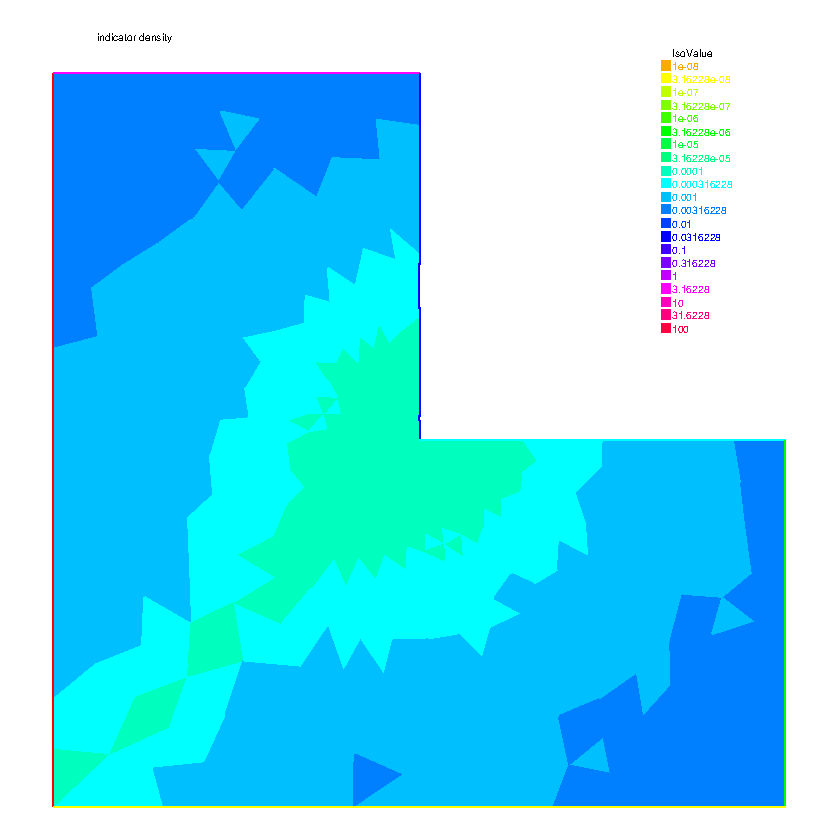
\includegraphics[height=8cm]{rhoP2} 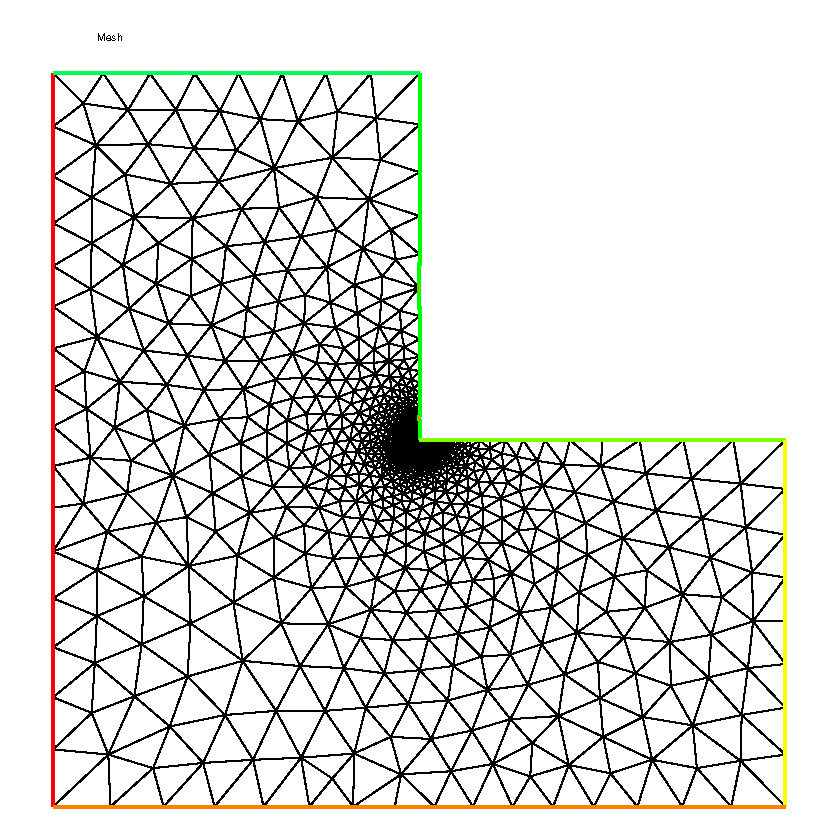
\includegraphics[height=8cm]{ThrhoP2}
\end{center}
\caption{Density of the error indicator  with isotropic $P^{2}$ metric }
\end{figure}
\subsection{Algo.edp}
We propose the solve the following non-linear academic  problem of minimization
of a functional $$J(u) = \int_\Omega f(|\nabla u|^2) - u*b $$
where $u$ is function of $H^1_0(\Omega)$.
and where $f$ is defined by
$$
f(x) = a*x + x-ln(1+x), \quad f'(x) = a+\frac{x}{1+x}, \quad f''(x) =  \frac{1}{(1+x)^2}
$$

\subsubsection{Non linear conjugate gradient algorithm}
\bFF

mesh Th=square(10,10);  // mesh definition of $\Omega$
fespace Vh(Th,P1);      // finite element space
fespace Ph(Th,P0);      // make optimization

\eFF
A small hack to construct a function 
$$Cl= \left\{\begin{array}{cl} 1 & \mbox{ on interior degree of freedom} \cr
 0 & \mbox{ on boundary degree of freedom} \end{array}\right. $$
\bFF
// Hack to construct an array :
//  1 on interior nodes and 0 on boundary nodes
varf vCl(u,v) = on(1,2,3,4,u=1);
Vh Cl;
Cl[]= vCl(0,Vh,tgv=1);  //  0 and tgv 
real tgv=Cl[].max;     // 
Cl[] = -Cl[];  Cl[] += tgv; Cl[] /=tgv;

 
\eFF
the definition of $f$, $f'$, $f''$ and $b$
\bFF
// $ J(u) = \int_\Omega f(|\nabla u|^2) - \int\Omega  u b $
// $ f(x) = a*x + x-ln(1+x), \quad f'(x) = a+\frac{x}{1+x}, \quad f''(x) =  \frac{1}{(1+x)^2}$
real a=0.001;

func real f(real u) { return u*a+u-log(1+u); }
func real df(real u) { return a+u/(1+u);}
func real ddf(real u) { return 1/((1+u)*(1+u));}
Vh b=1;  // to defined b
\eFF
the routine to compute the functional $J$
\bFF
func real J(real[int] & x)
  {
    Vh u;u[]=x; 
    real r=int2d(Th)(f( dx(u)*dx(u) + dy(u)*dy(u) ) - b*u) ;
    cout << "J(x) =" << r << " " << x.min <<  " " << x.max << endl;
    return r;
  }
\eFF
The function  \index{function}to compute $D J$, where $u$ is the current solution.
\bFF
Vh u=0; //  the current value of the solution
Vh alpha; // of store  $f(|\nabla u|^2)$
int iter=0;
alpha=df( dx(u)*dx(u) + dy(u)*dy(u) ); // optimization 

func real[int] dJ(real[int] & x)
  {
    int verb=verbosity; verbosity=0; 
    Vh u;u[]=x; 
    alpha=df( dx(u)*dx(u) + dy(u)*dy(u) ); // optimization 
    varf au(uh,vh) = int2d(Th)( alpha*( dx(u)*dx(vh) + dy(u)*dy(vh) ) - b*vh);
    x= au(0,Vh);  
    x = x.* Cl[]; //  the grad in 0 on boundary 
    verbosity=verb;
    return x; // warning no return of local array  
  }
\eFF

We want to construct also a preconditionner function $C$
with solving the problem:  find $u_h \in V_{0h}$ such that
$$\forall v_h \in V_{0h}, \quad  \int_\Omega \alpha \nabla u_h . \nabla vh = \int_\Omega b v_h  $$
where $ \alpha=f(|\nabla u|^2)$.
\bFF
varf alap(uh,vh,solver=Cholesky,init=iter)=  
   int2d(Th)( alpha *( dx(uh)*dx(vh) + dy(uh)*dy(vh) ))   + on(1,2,3,4,uh=0);

varf amass(uh,vh,solver=Cholesky,init=iter)=  int2d(Th)( uh*vh)  + on(1,2,3,4,uh=0);

matrix Amass = alap(Vh,Vh,solver=CG); // \index{matrix}

matrix Alap=  alap(Vh,Vh,solver=Cholesky,factorize=1);   // \index{Cholesky}\index{factorize=}\index{solver=}

// the preconditionner function
func real[int] C(real[int] & x)
{
   real[int] u(x.n);
   u=Amass*x;
   x = Alap^-1*u; 
   x = x .* Cl[];     
   return x; // no return of local array  variable 
}
\eFF

A good idea the solve the problem, is make 10 iteration of the conjugate gradient, 
recompute de preconditonner and restart the conjugate gradient:
\bFF
   verbosity=5;
   int conv=0;
   real eps=1e-6; 
   for(int i=0;i<20;i++)
   {
     conv=NLCG(dJ,u[],nbiter=10,precon=C,veps=eps); // \index{veps=}\index{NLCG}
     if (conv) break;  // if converge break loop
    
     alpha=df( dx(u)*dx(u) + dy(u)*dy(u) ); // recompute alpha optimization 
     Alap = alap(Vh,Vh,solver=Cholesky,factorize=1);   
     cout << " restart with new preconditionner " << conv << " eps =" << eps << endl;
   }

   plot (u,wait=1,cmm="solution with NLCG");
\eFF
{\bf Remark:} the keycode  \texttt{veps=eps} change the value of the current \texttt{eps}, this is
usefule in this case, because at the first iteration  the value of \texttt{eps} is change 
to $-$ the absolute stop test and we save this initial stop test of for the all process. We remove the problem
of the relative stop test in iterative procedure, because we start close to the solution
and  the relative stop test become very hard  to reach.

\subsubsection{Newton Ralphson algorithm}


Now, we solve the problem with Newton Ralphson algorithm, to solve the 
Euler problem $ \nabla J (u) = 0$
the algorithme is 
  $$ u^{n+1} = u^n - ( \nabla^2 J (u^{n})^{-1}*dJ(u^n) $$ 

\index{Newton}
First we introduice the two variational form \texttt{vdJ} and \texttt{vhJ} to
compute respectively $ \nabla J$ and $ \nabla^2 J$
\bFF
//   methode of  Newton Ralphson to solve dJ(u)=0;
//    $$ u^{n+1} = u^n - (\frac{\partial dJ}{\partial u_i})^{-1}*dJ(u^n) $$ 
//   ---------------------------------------------
  Ph dalpha ; //to store = $f''( |\nabla u|^2) $  optimisation


  // the variational form of evaluate  dJ = $ \nabla J$
  // --------------------------------------
  //  dJ =  f'()*( dx(u)*dx(vh) + dy(u)*dy(vh) 
  @varf vdJ(uh,vh) =  int2d(Th)( alpha*( dx(u)*dx(vh) + dy(u)*dy(vh) ) - b*vh)
  + on(1,2,3,4, uh=0);


  // the variational form of evaluate  ddJ   $= \nabla^2 J$ 
  // hJ(uh,vh) =  f'()*( dx(uh)*dx(vh) + dy(uh)*dy(vh)
  //            + f''()( dx(u)*dx(uh) + dy(u)*dy(uh) ) * (dx(u)*dx(vh) + dy(u)*dy(vh)) 
  @varf vhJ(uh,vh) = int2d(Th)( alpha*( dx(uh)*dx(vh) + dy(uh)*dy(vh) )
   +  dalpha*( dx(u)*dx(vh) + dy(u)*dy(vh)  )*( dx(u)*dx(uh) + dy(u)*dy(uh) ) )
   + on(1,2,3,4, uh=0);
   
 // the Newton algorithm
  Vh v,w; 
  u=0;
  @for (int i=0;i<100;i++)
   {
    alpha = df( dx(u)*dx(u) + dy(u)*dy(u) ) ; // optimization
    dalpha = ddf( dx(u)*dx(u) + dy(u)*dy(u) ) ; // optimization
    v[]= vdJ(0,Vh);  // $ v = \nabla J(u) $
    real res= v[]'*v[]; // the dot product 
    cout << i <<  " residu^2 = " <<  res  << endl;
    @if( res< 1e-12) @break;
    @matrix H= vhJ(Vh,Vh,factorize=1,solver=LU); //\index{matrix!factorize=}
    w[]=H^-1*v[];
    u[] -= w[];
   }
   plot (u,wait=1,cmm="solution with Newton Ralphson");
\eFF


\subsection{Stokes and Navier-Stokes}

  The Stokes equations are:
\index{stokes}
\Blue{
\begin{equation} \label{eq Stokes}
    \left.\begin{array}{cl}
 -\Delta u+\nabla p & =0 \\
 \nabla\cdot u &=0
 \end{array}\right\}\quad \hbox{ in }\Omega
\end{equation}
}
where $u$ is the velocity vector and $p$ the pressure.
For simplicity, let us choose Dirichlet boundary conditions
on the velocity,  $u=u_{\Gamma}$ on $\Gamma$.

A classical way to discretize the Stokes equation with a mixed formulation,
is to solve the variational problem and then discretize it:

Find $(u_{h},p_{h}) \in X_{h}^2 � M_{h}$ such that $u_{h} = u_{\Gamma h}$,
and such that
\Blue{
\begin{equation} \label{eq vf Stokes}
    \begin{array}{cll}
   \displaystyle \int_{\Omega_{h}} \nabla u_{h} \cdot  \nabla v_{h}  + \int \nabla p_{h} \cdot v_{h}  &= 0,
      &\forall v_{h} \in X_{0h} \\
    \displaystyle\int_{\Omega_{h}} \nabla.u_{h} q_{h} &= 0,
     &\forall q_{h} \in M_{h}
    \end{array}
\end{equation}
}
where $X_{0h}$ is the space of functions of $X_{h}$
which are zero on $\Gamma$.
The velocity space is approximated by  $X_{h}$ space, and
the pressure space is approximated by  $M_{h}$ space.


\subsubsection{Cavity.edp}


\medskip

The driven cavity flow problem is solved first at zero Reynolds number
(Stokes flow) and then at Reynolds 100.  \index{fluid}The
velocity pressure formulation is used first and then the calculation
is repeated with the stream function vorticity formulation.


The driven cavity problem is the problem (\ref{eq Stokes}) \index{Stokes} where
 $u_{\Gamma}\cdot n=0$ and $u_{\Gamma}\cdot s
=1$ on the top boundary and zero elsewhere ( $n$ is  the $\Gamma$ normal, and
 $s$ is the $\Gamma$ tangent).
\\
The mesh is constructed by
\bFF
@mesh Th=@square(8,8);
\eFF
The labels assigned by \texttt{square}
to the bottom,right,up and left edges are respectively $1,2,3,4$.

We use a classical Taylor-Hood element technic to solve the problem:
\\\\
The velocity is approximated with the $P_{2}$ FE ( $X_{h}$ space), and the
the pressure is approximated with the $P_{1}$ FE ( $M_{h}$ space),
\\\\
where
\Blue{
$$  X_{h} = \{ v \in H^{1}(]0,1[^2) \SE \forall K \in \mathcal{T}_{h}
\quad v_{|K} \in
P_{2} \}$$} and
\Blue{$$  M_{h} = \{ v \in H^{1}(]0,1[^2) \SE \forall K \in \mathcal{T}_{h}
\quad v_{|K} \in
P_{1} \}$$}

The FE spaces and functions  are constructed by

\bFF
@fespace Xh(Th,@P2); //  definition of the velocity component space
@fespace Mh(Th,@P1);  //  definition of the pressure space
Xh u2,v2;
Xh u1,v1;
Xh p,q;
\eFF

The Stokes operator is implemented as a system-solve for the velocity
$(u1,u2)$ and the pressure $p$.  The test function  for the velocity is $(v1,v2)$
and $q$ for the pressure, so the variational form (\ref{eq vf Stokes}) in freefem
language is:
\bFF
@solve Stokes (u1,u2,p,v1,v2,q,solver=Crout) =
    @int2d(Th)( ( dx(u1)*dx(v1) + dy(u1)*dy(v1)
            +  dx(u2)*dx(v2) + dy(u2)*dy(v2) )
            + p*q*(0.000001)
            + p*dx(v1)+ p*dy(v2)
            + dx(u1)*q+ dy(u2)*q
           )
  + @on(3,u1=1,u2=0)
  + @on(1,2,4,u1=0,u2=0);
\eFF
Each unknown has its own boundary conditions.
\\\\
{\bf Technical Remark}
There is some arbitrary decision here as to where to affect the
boundary condition within the linear system. Basically the Dirichlet
operator \index{Dirichlet}
(\texttt{on})  should be
associated with the unknown  which contains it so that
the penalization appears on the diagonal
of the matrix of the underlying discrete linear system,
otherwise it will be ill conditioned.
\index{Neumann}

\begin{note}
Notice the term \texttt{p*q*(0.000001)}  is added, because the  solver
Crout needs it: all the sub-matrices must be invertible.
\end{note}

If the \index{streamlines}streamlines are required, they can be
computed by finding $\psi$ such that rot$\psi=u$ or better,
\Blue{$$-\Delta\psi=\nabla� u$$}
\bFF
Xh psi,phi;

@solve streamlines(psi,phi) =
      @int2d(Th)( dx(psi)*dx(phi) + dy(psi)*dy(phi))
   +  @int2d(Th)( -phi*(dy(u1)-dx(u2)))
   +  @on(1,2,3,4,psi=0);
\eFF

\bigskip

Now the Navier-Stokes equations are solved
\eq{
    {\partial {u}\over\partial t} +u\cdot\nabla u-\nu \Delta u+\nabla p=0,~~~ \nabla\cdot u=0
}
with the same boundary conditions and with initial conditions $u=0$.

This is implemented by using the convection operator \texttt{convect} for the term
${\partial u\over\partial t} +u\cdot\nabla u$, giving a discretization in time
\Blue{\index{Navier-Stokes}
\begin{equation}
    \label{eq Navier Stokes carac}
\begin{array}{cl}
\frac{1}{\delta t} (u^{n+1}-u^n\circ X^n) -\nu\Delta u^{n+1} + \nabla p^{n+1} &=0,\\
 \nabla\cdot u^{n+1} &= 0
 \end{array}
\end{equation}
}
The term,$u^n\circ X^n(x)\approx u^n(x-u^n(x)\delta t)$ will be
computed by the operator ``convect" \index{convect} , so we obtain
\bFF
int i=0;
@real  nu=1./100.;
@real dt=0.1;
@real alpha=1/dt;

Xh up1,up2;

@problem  NS (u1,u2,p,v1,v2,q,solver=Crout,init=i) =
    @int2d(Th)(
             alpha*( u1*v1 + u2*v2)
            + nu * ( dx(u1)*dx(v1) + dy(u1)*dy(v1)
            +  dx(u2)*dx(v2) + dy(u2)*dy(v2) )
            + p*q*(0.000001)
            + p*dx(v1)+ p*dy(v2)
            + dx(u1)*q+ dy(u2)*q
           )
  + @int2d(Th) ( -alpha*
       convect([up1,up2],-dt,up1)*v1 -alpha*convect([up1,up2],-dt,up2)*v2 )
  + @on(3,u1=1,u2=0)
  + @on(1,2,4,u1=0,u2=0)
;

@for (i=0;i<=10;i++)
 {
   up1=u1;
   up2=u2;
   NS;
   @if ( !(i % 10))  // plot every 10 iteration
    @plot(coef=0.2,cmm=" [u1,u2] et p  ",p,[u1,u2]);
 } ;
\eFF
Notice that the matrices are \index{Reusable matrices} reused (keyword
\texttt{init=i})

\subsubsection{StokesUzawa.edp}

In this example we have a full Stokes problem, solve also the cavity problem,
with the
classical \index{Uzawa}\label{Uzawa} Uzawa conjugate gradient.

The idea of the algorithm is very simple, in the first equation of the Stokes problem, if
we know the pressure, when we can compute the velocity $u(p)$, and to solve
the problem is to find $p$, such that $ \nabla. u(p) =0$. The last problem is
linear, symmetric negative, so we can use the conjugate gradient algoritm \index{LinearCG}
.

First we define mesh, and the Taylor-Hood \index{Taylor-Hood}  approximation.
So $X_{h}$  is the velocity space, and $M_{h}$ is the pressure space.

\bFF
@mesh Th=@square(10,10);
@fespace Xh(Th,@P2),Mh(Th,@P1);
Xh u1,u2,v1,v2;
Mh p,q,ppp;  //  ppp is a working pressure
\eFF

\bFF
@varf bx(u1,q) = @int2d(Th)( -(dx(u1)*q));
@varf by(u1,q) = @int2d(Th)( -(dy(u1)*q));
@varf a(u1,u2)= @int2d(Th)(  dx(u1)*dx(u2) + dy(u1)*dy(u2) )
                    +  on(3,u1=1)  +  @on(1,2,4,u1=0) ;
//  remark:  put the \ttCC{@on(3,u1=1)} before  \ttCC{@on(1,2,4,u1=0)} 
//  because we want zero on intersection \index{on!intersection}
 
@matrix A= a(Xh,Xh,solver=CG);
@matrix Bx= bx(Xh,Mh);
@matrix By= by(Xh,Mh);

Xh bc1; bc1[] = a(0,Xh);  //  boundary condition contribution  on u1
Xh bc2; bc2   = O ;       //  no boundary condition contribution on u2
Xh b;
\eFF

Construct the function \texttt{divup} $ p \longrightarrow \nabla. u(p) $.
\bFF
@func @real[@int] divup(@real[@int] @& pp)
{
   //  compute u1(pp)
   b[]  = Bx'*pp; b[] += bc1[] ;    u1[] = A^-1*b[];
   //  compute u2(pp)
   b[]  = By'*pp; b[] += bc2[] ;    u2[] = A^-1*b[];
   //  div(u1,u2) = Bx'*u1[] + By'*u2[];
   ppp[] =   Bx*u1[];   // $  ppp= {}^t B_{x} u_{1} $ 
   ppp[] +=  By*u2[];   // $   \quad   +  {}^t B_{y} u_{2} $ 
   @return ppp[] ;
};
\eFF

 Call now the conjugate gradient algorithm:

\bFF
p=0;q=0;
@LinearCG(divup,p[],eps=1.e-6,nbiter=50);
divup(p[]); // compute the final solution

@plot([u1,u2],p,wait=1,value=true,coef=0.1);
\eFF

\subsubsection{NSUzawaCahouetChabart.edp}

 In this example we solve the Navier-Stokes \index{Navier-Stokes} equation,
 in the driven-cavity,
 with the Uzawa  algorithm preconditioned by the Cahouet-Chabart method.

 The idea of the preconditionner is that in a periodic domain, all
 differential operators commute and  the  Uzawa algorithm comes to solving the
 linear operator  $ \nabla. ( (\alpha Id + \nu \Delta)^{-1} \nabla$,
 where $ Id $ is the identity operator.
 So  the preconditioner suggested is $ \alpha \Delta^{-1} + \nu Id$.
\\\\
To implement this, we reuse the previous example, by including \index{include} a file.
Then we define the time step $ \Delta t$, viscosity, and new variational form, and matrix.

\bFF
@include "StokesUzawa.edp" // include the Stokes part
@real dt=0.05, alpha=1/dt;  // $ \Delta t$

@cout << " alpha = " << alpha;
@real xnu=1./400; // viscosity $ \nu = {\hbox{Reynolds number}}^{-1} $

//  the new variational form with mass term \index{varf}
@varf at(u1,u2)= @int2d(Th)( xnu*dx(u1)*dx(u2)
                        + xnu*dy(u1)*dy(u2) + u1*u2*alpha  )
                        +  @on(1,2,4,u1=0)  + @on(3,u1=1) ;

A = at(Xh,Xh,solver=CG);  //  change the matrix \index{matrix!=}\index{matrix!solver=}

//  set the 2 convect variational form \index{qforder=} \index{convect}
@varf  vfconv1(uu,vv)  = @int2d(Th,qforder=5) (@convect([u1,u2],-dt,u1)*vv*alpha);
@varf  vfconv2(v2,v1)  = @int2d(Th,qforder=5) (@convect([u1,u2],-dt,u2)*v1*alpha);

@int idt;       // index of of time set
@real temps=0;  // current time

Mh pprec,prhs;
@varf vfMass(p,q) = int2d(Th)(p*q);
@matrix MassMh=vfMass(Mh,Mh,solver=CG);

@varf vfLap(p,q)  = int2d(Th)(dx(pprec)*dx(q)+dy(pprec)*dy(q) + pprec*q*1e-10);
@matrix LapMh= vfLap(Mh,Mh,solver=Cholesky);
\eFF

 The function to define the preconditioner

\bFF
func real[int]  CahouetChabart(real[int] & xx)
{  //  xx = $ \int (div u) w_i$
   //   $ \alpha LapMh ^{-1}  + \nu MassMh^{-1} $ 
   pprec[]= LapMh^-1* xx; 
   prhs[] =  MassMh^-1*xx;
   pprec[] = alpha*pprec[]+xnu* prhs[];
   return pprec[];
};
\eFF

The loop in time.
Warning with the stop test of the conjugate gradient, because
we start from the previous solution and the end the previous solution
is close to the final solution, don't take a relative  stop test to
the first residual, take an absolue stop test ( negative here)
\index{stop test!absolue}
\bFF
for (idt = 1; idt < 50; idt++)
 {
   temps += dt;
   cout << " --------- temps " << temps << " \n ";
   b1[] =  vfconv1(0,Xh);
   b2[] =  vfconv2(0,Xh);
   cout << "  min b1 b2  " << b1[].min << " " << b2[].min << endl;
   cout << "  max b1 b2  " << b1[].max << " " << b2[].max << endl;
   // call Conjugued Gradient with preconditioner '
   //  warning eps < 0 => absolue stop test \index{precon=}
   LinearCG(divup,p[],eps=-1.e-6,nbiter=50,precon=CahouetChabart);
   divup(p[]);   //  computed the velocity

   plot([u1,u2],p,wait=!(idt%10),value= 1,coef=0.1);
 }
\eFF


\subsection{Readmesh.edp}
\index{read files}
\index{write files}
Freefem can read and write files which can be reused once read but the
names of the borders are lost and they have to be replaced by the number
which corresponds to their order of appearance in the program, unless
the number is forced by the keyword "label".
\bFF
@border floor(t=0,1){ x=t; y=0; label=1;}; // the unit square
@border right(t=0,1){ x=1; y=t; label=5;};
@border ceiling(t=1,0){ x=t; y=1; label=5;};
@border left(t=1,0){ x=0; y=t; label=5;};
@int n=10;
@mesh th= buildmesh(floor(n)+right(n)+ceiling(n)+left(n));
@savemesh(th,"toto.am_fmt");  // format "formated Marrocco" \index{file!am\_fmt}
@savemesh(th,"toto.Th");      // format database  db mesh "bamg"   \index{file!bamg}
@savemesh(th,"toto.msh");     // format freefem \index{file!mesh}
@savemesh(th,"toto.nopo");     // modulef format \index{file!nopo} see \cite{modulef}
@mesh th2 = readmesh("toto.msh");
@fespace femp1(th,@P1);
femp1 f = sin(x)*cos(y),g;
{ // save solution
@ofstream file("f.txt");
file << f[] << endl;
}  // close the file (end block)
{  // read
@ifstream file("f.txt");
file >> g[] ;
} // close reading file (end block)
@fespace Vh2(th2,P1);
Vh2 u,v;
@plot(g);
@solve pb(u,v) =
    @int2d(th)( u*v - dx(u)*dx(v)-dy(u)*dy(v) )
  + @int2d(th)(-g*v)
  + @int1d(th,5)( g*v)
  + @on(1,u=0) ;
@plot (th2,u);
\eFF

There are many formats of mesh files available for communication with other tools such as
emc2, modulef..., the suffix gives the chosen type.\index{bamg}
More details can be found in the article by F. Hecht "bamg : a bidimentional
anisotropic mesh generator"  available from the freefem web page.
\\
Note also the wrong sign in the Laplace equation, but freefem can handle it as long as it
is not a resonance mode (i.e. the matrix of the linear system should be non-singular).
\subsection{Domain decomposition}
We present, three classique examples, of domain decomposition
technique:
first, Schwarz algorithm with overlapping, second 
Schwarz algorithm without  overlapping (also call Shur complement), and
last we show to use the conjugate gradient 
to solve the boundary problem of the Shur complement.
 
\subsubsection{Schwarz-overlap.edp}\label{schwarz-overlap}
To solve 
\eq{ -\Delta u =f,\; \hin\Omega=\Omega_1\cup\Omega_2\quad u|_\Gamma=0}
the Schwarz algorithm  runs like this
\eq{
    -\Delta u^{m+1}_1=f\hin\Omega_1\quad
    u^{m+1}_1|_{\Gamma_1}=u^m_2
 }
\eq{
    -\Delta u^{m+1}_2=f\hin\Omega_2\quad
    u^{m+1}_2|_{\Gamma_2}=u^m_1
}
 where $\Gamma_i$ is the boundary of $\Omega_i$ and on the
condition that $\Omega_1\cap\Omega_2\neq\emptyset$ and that $u_i$
are zero at iteration 1.
\\\\
Here we take $\Omega_1$ to be a quadrangle, $\Omega_2$ a disk and
we apply the algorithm starting from zero.
\begin{figure}[hbt]
\HLINE{\hss
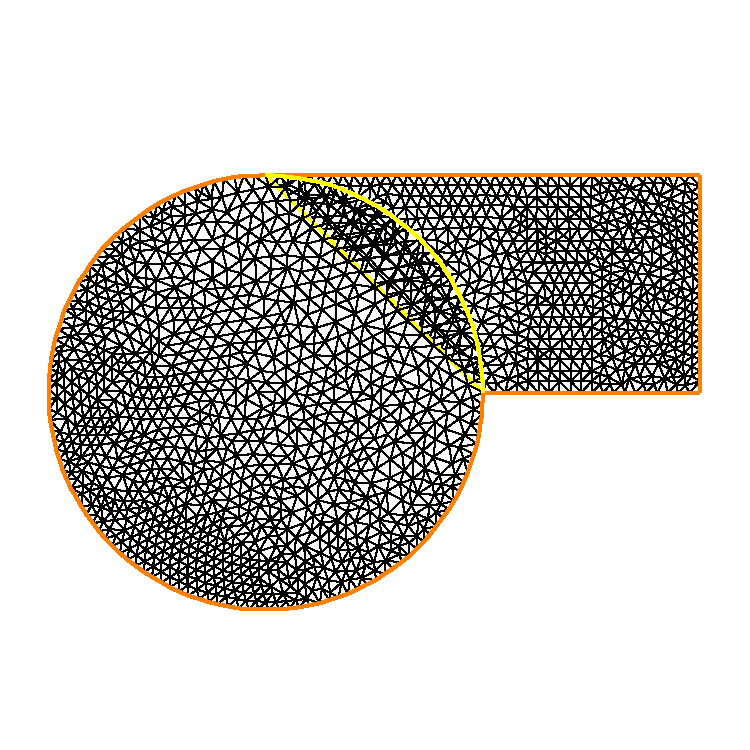
\includegraphics[width=6cm]{schwarz-th} \hss}
\caption{ The 2 overlapping mesh \texttt{TH} and \texttt{th}  }
\end{figure}

 \bFF
@int inside = 2;  //  inside boundary
@int outside = 1; //  outside boundary
@border a(t=1,2){x=t;y=0;label=outside;};
@border b(t=0,1){x=2;y=t;label=outside;};
@border c(t=2,0){x=t ;y=1;label=outside;};
@border d(t=1,0){x = 1-t; y = t;label=inside;};
@border e(t=0, pi/2){ x= cos(t); y = sin(t);label=inside;};
@border e1(t=pi/2, 2*pi){ x= cos(t); y = sin(t);label=outside;};
@int n=4;
@mesh th = @buildmesh( a(5*n) + b(5*n) + c(10*n) + d(5*n));
@mesh TH = @buildmesh( e(5*n) + e1(25*n) );
@plot(th,TH,wait=1);  //  to see the 2 meshes
\eFF

The space  and problem definition is :   
\bFF
@fespace vh(th,@P1);
@fespace VH(TH,@P1);
vh u=0,v; VH U,V;
@int i=0;

@problem PB(U,V,init=i,solver=Cholesky) = 
    @int2d(TH)( dx(U)*dx(V)+dy(U)*dy(V) )
  + @int2d(TH)( -V) + on(inside,U = u)  + @on(outside,U= 0 ) ;
@problem pb(u,v,init=i,solver=Cholesky) =
    @int2d(th)( dx(u)*dx(v)+dy(u)*dy(v) )
  + @int2d(th)( -v) + on(inside ,u = U) + @on(outside,u = 0 ) ;
\eFF
 The  calculation loop: 
\bFF
@for ( i=0 ;i< 10; i++)
{
   PB;
   pb;
   @plot(U,u,wait=true);
};
\eFF


\begin{figure}[hbt]
\HLINE{\hss
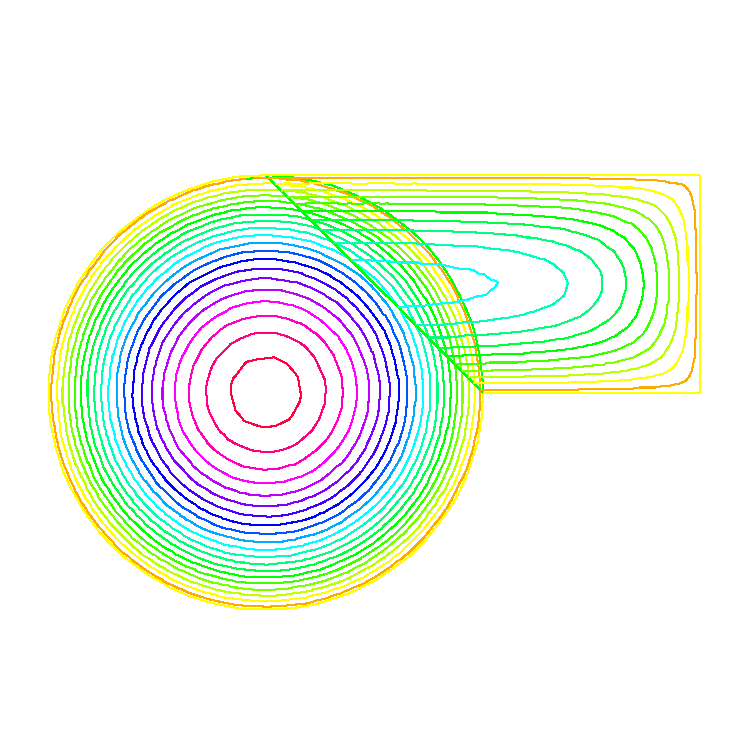
\includegraphics[width=6cm]{schwarz-u0} 
\hss
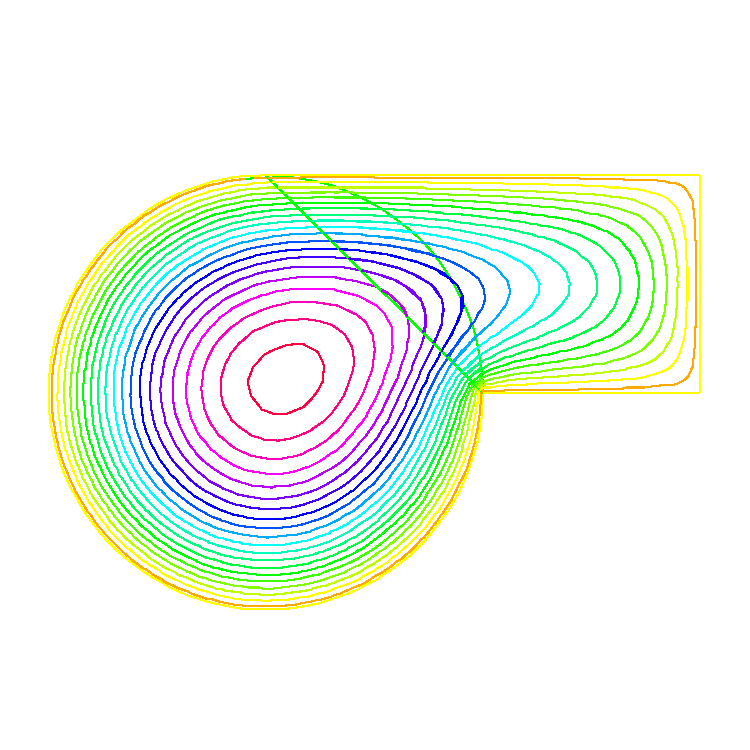
\includegraphics[width=6cm]{schwarz-u} }
\caption{  Isovalues of the solution at  iteration 0  and iteration 9}
\end{figure}



\subsubsection{Schwarz-no-overlap.edp}

To solve\index{domain decomposition}\index{shurr}
\eq{ -\Delta u =f \hin\Omega=\Omega_1\cup\Omega_2\quad u|_\Gamma=0,}
the Schwarz algorithm for domain decomposition without overlapping  runs like this

\begin{figure}[hbt]
\HLINE{\hss
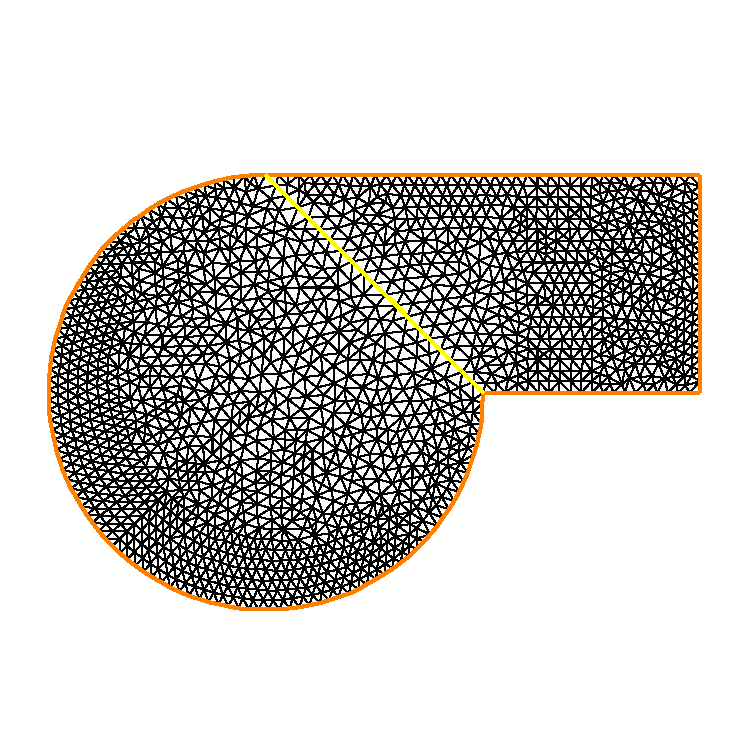
\includegraphics[width=6cm]{schwarz-no-th} \hss}
\caption{ The two none overlapping mesh \texttt{TH} and \texttt{th}  }
\end{figure}

Let introduce  $\Gamma_i$ is  common the boundary of $\Omega_1$ and
$\Omega_2$ and    $\Gamma_e^i= \partial \Omega_i \setminus \Gamma_i$.

The probem  find  $\lambda$ such that $ (u_1|_{\Gamma_i}=u_2|_{\Gamma_i}) $
where  $u_i$ is solution of the following Laplace problem:
\eq{
    -\Delta u_i=f\hin\Omega_i\quad
    u_i|_{\Gamma_i}=\lambda \quad
    u_i|_{\Gamma_e^i} = 0 
 }

To solve this problem we just make a loop
with upgrading$\lambda$ with
$$\lambda = \lambda � \frac{(u_1-u_2)}{2}$$
where the sign $+$ or $-$ of $�$ is choose to have convergence.

\bFF
// schwarz1 without overlapping
@int inside = 2;
@int outside = 1;
@border a(t=1,2){x=t;y=0;label=outside;};
@border b(t=0,1){x=2;y=t;label=outside;};
@border c(t=2,0){x=t ;y=1;label=outside;};
@border d(t=1,0){x = 1-t; y = t;label=inside;};
@border e(t=0, 1){ x= 1-t; y = t;label=inside;};
@border e1(t=pi/2, 2*pi){ x= cos(t); y = sin(t);label=outside;}; 
@int n=4;
@mesh th = buildmesh( a(5*n) + b(5*n) + c(10*n) + d(5*n));
@mesh TH = buildmesh ( e(5*n) + e1(25*n) );
@plot(th,TH,wait=1,ps="schwarz-no-u.eps");
@fespace vh(th,P1);
@fespace VH(TH,P1);
vh u=0,v; VH U,V;
vh lambda=0;
@int i=0;

@problem PB(U,V,init=i,solver=Cholesky) = 
    @int2d(TH)( dx(U)*dx(V)+dy(U)*dy(V) )
  + @int2d(TH)( -V) 
  + @int1d(TH,inside)(-lambda*V) +    on(outside,U= 0 ) ;
@problem pb(u,v,init=i,solver=Cholesky) = 
    @int2d(th)( dx(u)*dx(v)+dy(u)*dy(v) )
  + @int2d(th)( -v) 
  + @int1d(th,inside)(+lambda*v) +    on(outside,u = 0 ) ;


@for ( i=0 ;i< 10; i++) 
{   
   PB; 
   pb;
   lambda = lambda - (u-U)/2;
   @plot(U,u,wait=true);
};

@plot(U,u,ps="schwarz-no-u.eps");

\eFF

\begin{figure}[hbt]
\HLINE{\hss
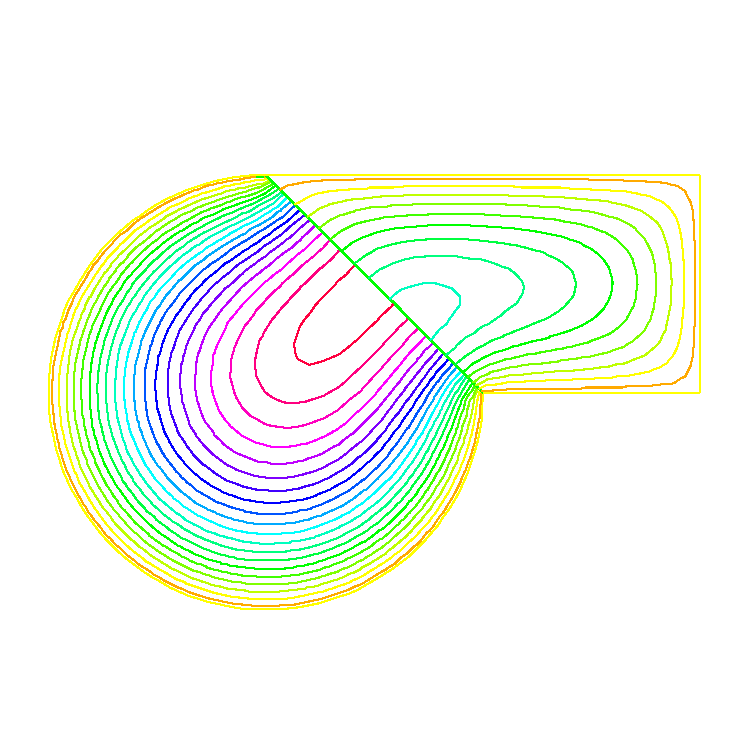
\includegraphics[width=6cm]{schwarz-no-u0} 
\hss
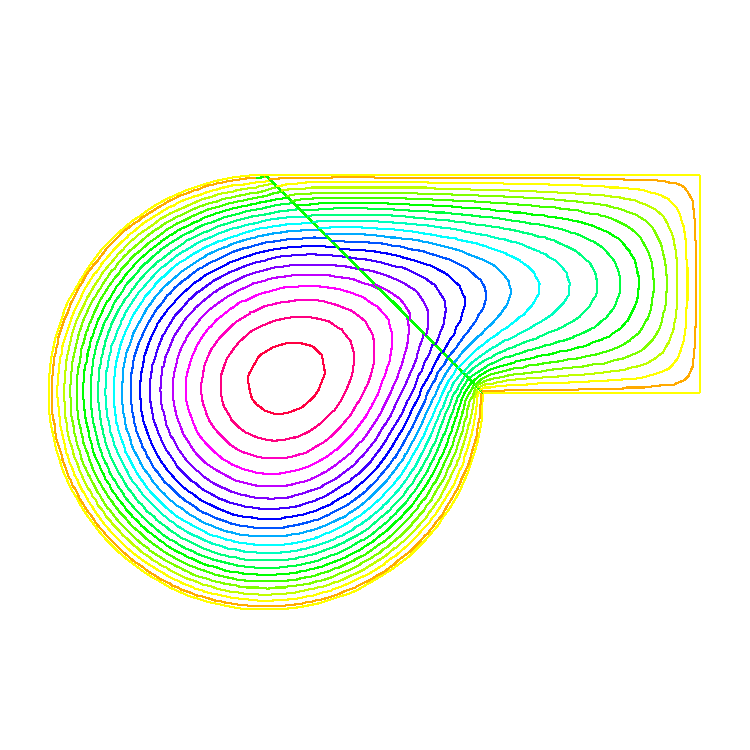
\includegraphics[width=6cm]{schwarz-no-u} }
\caption{  Isovalues of the solution at  iteration 0  and iteration 9 without overlapping }
\end{figure}

\subsubsection{Schwarz-gc.edp}
To solve\index{domain decomposition}\index{shurr}
\eq{ -\Delta u =f \hin\Omega=\Omega_1\cup\Omega_2\quad u|_\Gamma=0,}
the Schwarz algorithm for domain decomposition without overlapping  runs like this

Let introduce  $\Gamma_i$ is  common the boundary of $\Omega_1$ and
$\Omega_2$ and    $\Gamma_e^i= \partial \Omega_i \setminus  \Gamma_i$.

The probem  find  $\lambda$ such that $ (u_1|_{\Gamma_i}=u_2|_{\Gamma_i}) $
where  $u_i$ is solution of the following Laplace problem:
\eq{
    -\Delta u_i=f\hin\Omega_i\quad
    u_i|_{\Gamma_i}=\lambda \quad
    u_i|_{\Gamma_e^i} = 0 
 }

The version of this example for  Shur componant. The border problem
is solve with conjugate gradient. 

First, we construct the two domain 
\bFF
// Schwarz without overlapping (Shur complenement Neumann -> Dirichet)  
@real cpu=clock();
@int inside = 2; 
@int outside = 1; 

@border Gamma1(t=1,2){x=t;y=0;label=outside;};
@border Gamma2(t=0,1){x=2;y=t;label=outside;};
@border Gamma3(t=2,0){x=t ;y=1;label=outside;};

@border GammaInside(t=1,0){x = 1-t; y = t;label=inside;};

@border GammaArc(t=pi/2, 2*pi){ x= cos(t); y = sin(t);label=outside;}; 
int n=4;
//  build the mesh of $\Omega_1$ and $\Omega_2$
@mesh Th1 = buildmesh( Gamma1(5*n) + Gamma2(5*n) + GammaInside(5*n) + Gamma3(5*n));
@mesh Th2 = buildmesh ( GammaInside(-5*n) + GammaArc(25*n) );
@plot(Th1,Th2);

// defined the 2 FE space
@fespace Vh1(Th1,P1),      Vh2(Th2,P1);
\eFF
Remark, to day is not possible to
defined a function just on a border, so the $\ lambda $
function is defined on the all domain $\Omega_1$
by:

\bFF
@Vh1 lambda=0;  // take $\lambda \in V_{h1}$
\eFF
The two Laplace problem:
\bFF
@Vh1 u1,v1;              Vh2 u2,v2;
@int i=0;  // for factorization optimization 
@problem Pb2(u2,v2,init=i,solver=Cholesky) = 
    int2d(Th2)( dx(u2)*dx(v2)+dy(u2)*dy(v2) )
  + int2d(Th2)( -v2) 
  + int1d(Th2,inside)(-lambda*v2) +    on(outside,u2= 0 ) ;
@problem Pb1(u1,v1,init=i,solver=Cholesky) = 
    int2d(Th1)( dx(u1)*dx(v1)+dy(u1)*dy(v1) )
  + int2d(Th1)( -v1) 
  + int1d(Th1,inside)(+lambda*v1) +    on(outside,u1 = 0 ) ;
\eFF

Now, we define a border matrix , because the
 $\ lambda $ function is none zero inside the domain $\Omega_1$:
\bFF
@varf b(u2,v2,solver=CG) =int1d(Th1,inside)(u2*v2);
@matrix B= b(Vh1,Vh1,solver=CG);
\eFF

The boundary problem function,
  $$
  \lambda \longrightarrow  \int_{\Gamma_i }(u_1-u_2) v_{1}
$$
\bFF
@func @real[@int] BoundaryProblem(real[int] &l)
{ 
   lambda[]=l; // make FE function form l
   Pb1;     Pb2;
   i++;  //  no  refactorization i !=0
   v1=-(u1-u2); 
   lambda[]=B*v1[];
   @return lambda[] ;
};
\eFF
Remark, the  difference between the two notations \ttCC{v1} and \ttCC{v1[]}  is: 
 \ttCC{v1} is the finite element  function and \ttCC{v1[]} 
is the vector in the canonical basis of the   finite element  function  \ttCC{v1} .
\index{[]@\verb=[]=}
 
\bFF
Vh1 p=0,q=0; 
//  solve the problem with Conjugue Gradient
LinearCG(BoundaryProblem,p[],eps=1.e-6,nbiter=100);
//  compute the final solution, because CG works with increment
BoundaryProblem(p[]); // solve again  to have right u1,u2

cout << " -- CPU time  schwarz-gc:" <<  clock()-cpu << endl;
plot(u1,u2); // plot 
\eFF


\subsection{Beam.edp}

Elastic solids subject to forces deform: a point in the solid,
originaly at (x,y)
goes to (X,Y) after.  When the displacement vector
$\vec v=(v_1,v_2) = (X-x, Y-y)$  is small, Hooke's
law relates the stress tensor $\sigma$ inside the solid to the
deformation tensor $\epsilon$:
\Blue{
 $$ \sigma_{ij} = \lambda \delta_{ij} \nabla.\vec v + 2\mu\epsilon_{ij},
\,
\epsilon_{ij} = {1\over 2}({\partial v_i\over\partial x_j} +
{\partial v_j\over\partial x_i} )$$
}
where $\delta$ is the Kronecker symbol
and where $\lambda, \mu$ are two constants describing the material mechanical
properties in terms of the modulus of
elasticity, and Young's modulus.

The equations of elasticity are naturally written in variational form
for the displacement vector $v(x)\in V$ as
\Blue{$$
\int_\Omega [\mu\epsilon_{ij}(\vec v)\epsilon_{ij}(\vec w)
+\lambda \epsilon_{ii}(v)\epsilon_{jj}(\vec w)]
=\int_\Omega \vec g\cdot \vec w +\int_\Gamma \vec h\cdot \vec w,%\`{u}
\forall \vec w\in V
$$}

The  elastic solids  is a rectangle beam $[0,10]�[0,2]$.
The data are the gravity force $\vec g$ and the
boundary stress i$\vec h$ is zero on lower and upper side, and on the  two vertical sides of the beam are locked.
\bFF
//   a weighting beam sitting on a

int bottombeam = 2;
@border a(t=2,0)  { x=0; y=t ;label=1;};        //  left beam
@border b(t=0,10) { x=t; y=0 ;label=bottombeam;};        //  bottom of beam
@border c(t=0,2)  { x=10; y=t ;label=1;};       //  rigth beam
@border d(t=0,10) { x=10-t; y=2; label=3;};     //  top beam 
@real E = 21.5;
@real sigma = 0.29;
@real mu = E/(2*(1+sigma));
@real lambda = E*sigma/((1+sigma)*(1-2*sigma));
@real gravity = -0.05;
@mesh th = buildmesh( b(20)+c(5)+d(20)+a(5));
@fespace Vh(th,[P1,P1]);
Vh [uu,vv], [w,s];
@cout << "lambda,mu,gravity ="<<lambda<< " " << mu << " " << gravity << endl;
// deformation of a beam under its own weight 
@solve  bb([uu,vv],[w,s])  = 
    @int2d(th)(
                2*mu*(dx(uu)*dx(w)+dy(vv)*dy(s)+ ((dx(vv)+dy(uu))*(dx(s)+dy(w)))/2 )
               + lambda*(dx(uu)+dy(vv))*(dx(w)+dy(s))
             ) 
  + @int2d(th) (-gravity*s)
  + @on(1,uu=0,vv=0)
 ;


@plot([uu,vv],wait=1);
@plot([uu,vv],wait=1,bb=[[-0.5,2.5],[2.5,-0.5]]); 
@mesh th1 = movemesh(th, [x+uu, y+vv]);
@plot(th1,wait=1);
\eFF

\subsection{Fluidstruct.edp}
\index{fluid-structure interaction}


This problem involves the Lam� system of elasticity
and the Stokes system for viscous fluids with velocity $\vec u$ and pressure $p$:
\begin{eqnarray*}\Blue
-\Delta \vec u +\vec\nabla p = 0, \,
%\`{u}
\nabla\cdot \vec u = 0,\hbox{~~in ~}\Omega,\,
\vec u=\vec u_\Gamma \hbox{~~on~~}\Gamma=\partial\Omega
\end{eqnarray*}\Black
where $u_\Gamma$ is the velocity of the boundaries. The
force  that the fluid applies to the boundaries is the normal stress
\Blue{$$
\vec h =(\nabla\vec u +\nabla\vec u^T)\vec n -p\vec n
$$}

Elastic solids subject to forces deform: a point in the solid,
originaly at (x,y)
goes to (X,Y) after.  When the displacement vector
$\vec v=(v_1,v_2) = (X-x, Y-y)$  is small, Hooke's
law relates the stress tensor $\sigma$ inside the solid to the
deformation tensor $\epsilon$:
\Blue{
 $$ \sigma_{ij} = \lambda \delta_{ij} \nabla.\vec v + \mu\epsilon_{ij},
\,
\epsilon_{ij} = {1\over 2}({\partial v_i\over\partial x_j} +
{\partial v_j\over\partial x_i} )$$
}
where $\delta$ is the Kronecker symbol
and where $\lambda, \mu$ are two constants describing the material mechanical
properties in terms of the modulus of
elasticity, and Young's modulus.

The equations of elasticity are naturally written in variational form
for the displacement vector $v(x)\in V$ as
\Blue{$$
\int_\Omega [\mu\epsilon_{ij}(\vec v)\epsilon_{ij}(\vec w)
+\lambda \epsilon_{ii}(v)\epsilon_{jj}(\vec w)]
=\int_\Omega \vec g\cdot \vec w +\int_\Gamma \vec h\cdot \vec w,%\`{u}
\forall \vec w\in V
$$}
The data are the gravity force $\vec g$ and the
boundary stress $\vec h$.

In our example the Lam� system and the Stokes system are coupled by a
common boundary on which
the fluid  stress creates a displacement of the boundary and hence
changes the shape of the domain where the Stokes problem is integrated.
The geometry is that of a vertical driven cavity with an elastic lid.
The lid is a beam with weight so it will
be deformed by its own weight and by the normal stress due to the fluid reaction.
The cavity is the $10 � 10$ square and the lid is a rectangle of height $l=2$.
\\\\
A beam sits on a box full of fluid rotating because the left vertical side has velocity one.
The beam is bent by its own weight, but the pressure of the fluid modifies the bending.
\\
The bending displacement of the beam is given by (uu,vv) solution of
\bFF
//  Fluid-structure interaction for a weighting beam sitting on a
// square cavity filled with a fluid.

@int bottombeam = 2; // label of bottombeam
@border a(t=2,0)  { x=0; y=t ;label=1;};        //  left beam
@border b(t=0,10) { x=t; y=0 ;label=bottombeam;};        //  bottom of beam
@border c(t=0,2)  { x=10; y=t ;label=1;};       //  rigth beam
@border d(t=0,10) { x=10-t; y=2; label=3;};     //  top beam
@real E = 21.5;
@real sigma = 0.29;
@real mu = E/(2*(1+sigma));
@real lambda = E*sigma/((1+sigma)*(1-2*sigma));
@real gravity = -0.05;
@mesh th = @buildmesh( b(20)+c(5)+d(20)+a(5));
@fespace Vh(th,@P1);
Vh uu,w,vv,s,fluidforce=0;
@cout << "lambda,mu,gravity ="<<lambda<< " " << mu << " " << gravity << @endl;
// deformation of a beam under its own weight
@solve  bb([uu,vv],[w,s])  =
    @int2d(th)(
                 2*mu*(dx(uu)*dx(w)+ ((dx(vv)+dy(uu))*(dx(s)+dy(w)))/4 )
               + lambda*(dx(uu)+dy(vv))*(dx(w)+dy(s))/2
             )
  + @int2d(th) (-gravity*s)
  + @on(1,uu=0,vv=0)
  + fluidforce[];
 ;

 @plot([uu,vv],wait=1);
 @mesh th1 = movemesh(th, [x+uu, y+vv]);
 @plot(th1,wait=1);
\eFF
Then Stokes equation for fluids ast low speed are solved in the box below the beam,
but the beam has deformed the box (see border h):
\bFF
//Stokes on square  b,e,f,g  driven cavite on left side g
@border e(t=0,10) { x=t; y=-10; label= 1; };      //  bottom
@border f(t=0,10) { x=10; y=-10+t ; label= 1; };   //  right
@border g(t=0,10) { x=0; y=-t ;label= 2;};       //  left
@border h(t=0,10) { x=t; y=vv(t,0)*( t>=0.001 )*(t <= 9.999); 
                    label=3;};   //  top of cavity deforme

@mesh sh = @buildmesh(h(-20)+f(10)+e(10)+g(10));
@plot(sh,wait=1);
\eFF

 We use the Uzawa conjugate gradient to solve the Stokes problem like in example \ref{Uzawa}

\bFF
@fespace Xh(sh,P2),Mh(sh,P1);
Xh u1,u2,v1,v2;
Mh p,q,ppp;


@varf bx(u1,q) = @int2d(sh)( -(dx(u1)*q));

@varf by(u1,q) = @int2d(sh)( -(dy(u1)*q));

@varf Lap(u1,u2)= @int2d(sh)(  dx(u1)*dx(u2) + dy(u1)*dy(u2) )
                    +  @on(2,u1=1) +  @on(1,3,u1=0)  ;

Xh bc1; bc1[] = Lap(0,Xh);
Xh brhs;

@matrix A= Lap(Xh,Xh,solver=CG);
@matrix Bx= bx(Xh,Mh);
@matrix By= by(Xh,Mh);
Xh bcx=0,bcy=1;

@func @real[@int] divup(@real[@int] & pp)
{
  @int verb=verbosity;
   verbosity=0;
   brhs[]  = Bx'*pp; brhs[] += bc1[] .*bcx[];
   u1[] = A^-1*brhs[];
   brhs[]  = By'*pp; brhs[] += bc1[] .*bcy[];
   u2[] = A^-1*brhs[];
   ppp[] =   Bx*u1[];
   ppp[] +=  By*u2[];
   verbosity=verb;
   @return ppp[] ;
};

 p=0;q=0;u1=0;v1=0;

 @LinearCG(divup,p[],eps=1.e-3,nbiter=50);
 divup(p[]);
\eFF
Now the beam will feel the stress constraint from the fluid:
\bFF
  Vh sigma11,sigma22,sigma12;
  Vh uu1=uu,vv1=vv;

  sigma11([x+uu,y+vv]) = (2*dx(u1)-p);
  sigma22([x+uu,y+vv]) = (2*dy(u2)-p);
  sigma12([x+uu,y+vv]) = (dx(u1)+dy(u2));
\eFF
which comes as a boundary condition to the PDE of the beam:
\bFF
@varf fluidf([uu,vv],[w,s]) fluidforce =
@solve  bbst([uu,vv],[w,s],init=i)  =
    @int2d(th)(
                 2*mu*(dx(uu)*dx(w)+ ((dx(vv)+dy(uu))*(dx(s)+dy(w)))/4 )
               + lambda*(dx(uu)+dy(vv))*(dx(w)+dy(s))/2
             )
  + @int2d(th) (-gravity*s)
  + @int1d(th,bottombeam)( -coef*(   sigma11*N.x*w + sigma22*N.y*s 
                                   + sigma12*(N.y*w+N.x*s) )  )
  + @on(1,uu=0,vv=0);
 @plot([uu,vv],wait=1);
 @real  err = sqrt(@int2d(th)( (uu-uu1)^2 + (vv-vv1)^2 ));
 @cout <<  " Erreur L2 = " << err << "----------\n";
\eFF

Notice that the matrix generated by bbst is reused (see \ttCC{init=i}).
Finally we deform the beam
\bFF
 th1 = @movemesh(th, [x+0.2*uu, y+0.2*vv]);
 @plot(th1,wait=1);
\eFF
\subsection{Region.edp}
This example explains the definition and manipulation of \emph{region}, i.e.
\index{subdomains} subdomains of the whole domain.

Consider this L-shaped domain with 3 diagonals as internal boundaries, defining
4 subdomains:

\bFF
//   example using region keywork
// construct a mesh with 4 regions (sub-domains)
border a(t=0,1){x=t;y=0;};
border b(t=0,0.5){x=1;y=t;};
border c(t=0,0.5){x=1-t;y=0.5;};
border d(t=0.5,1){x=0.5;y=t;};
border e(t=0.5,1){x=1-t;y=1;};
border f(t=0,1){x=0;y=1-t;};
//  internal boundary 
border i1(t=0,0.5){x=t;y=1-t;};
border i2(t=0,0.5){x=t;y=t;};
border i3(t=0,0.5){x=1-t;y=t;};
   
mesh th = buildmesh (a(6) + b(4) + c(4) +d(4) + e(4) + 
    f(6)+i1(6)+i2(6)+i3(6));
fespace Ph(th,P0);  // constant discontinuous functions / element
fespace Vh(th,P1);  // $P_1$ ontinuous functions / element

Ph reg=region; //  defined the $P_0$ function  associed to region number 
plot(reg,fill=1,wait=1,value=1);
\eFF
\twoplot[height=8cm]{region}{region_nu}{the function \texttt{reg}}{the function \texttt{nu} }

\index{region} \texttt{region}  is a keyword of freefem++ which is in fact a variable depending of 
the current position (is not a function today, use \texttt{Ph reg=region;} to  set  a function).  This variable value returned is the number of the
subdomain of the current position.  This number is defined by "buildmesh" which scans while building the mesh all
its connected component.  So to get the number of a region containing a particular point
one does:
\bFF

int nupper=reg(0.4,0.9); // get the region number of point (0.4,0.9)
int nlower=reg(0.9,0.1);  // get the region number of point (0.4,0.1)
cout << " nlower " <<  nlower << ", nupper = " << nupper<< endl;
//  defined the characteristics functions of upper and lower region
Ph nu=1+5*(region==nlower) + 10*(region==nupper);
plot(nu,fill=1,wait=1);
\eFF
This is particularly useful to define \index{discontinuous functions}discontinuous functions such as might occur
when one part of the domain is copper and the other one is iron, for example.
\\
We this in mind we proceed to solve a Laplace equation with discontinuous coefficients
($\nu$ is 1, 6 and 11 below).
\bFF
Ph nu=1+5*(region==nlower) + 10*(region==nupper);
plot(nu,fill=1,wait=1);
problem lap(u,v) =   int2d(th)( dx(u)*dx(v)*dy(u)*dy(v)) + int2d(-1*v) + on(a,b,c,d,e,f,u=0);
plot(u);
\eFF
\plot[height=8cm]{region_u}{the isovalue of the solution $u$}
\newpage
\subsection{FreeBoundary.edp}

The domain $\Omega$ is defined with:

\bFF
@real L=10;        //longueur du domaine                                    
@real h=2.1;      // hauteur du bord gauche
@real h1=0.35;    // hauteur du bord droite

//  maillage d'un tapeze
@border a(t=0,L){x=t;y=0;};       // bottom:  $\Gamma_a$ \hfill              
@border b(t=0,h1){x=L;y=t;};      // right:  $\Gamma_b$ \hfill    
@border f(t=L,0){x=t;y=t*(h1-h)/L+h;}; //  free surface:  $\Gamma_f$ \hfill    
@border d(t=h,0){x=0;y=t;};      // left:  $\Gamma_d$ \hfill 

@int n=4;
@mesh Th=@buildmesh (a(10*n)+b(6*n)+f(8*n)+d(3*n));
@plot(Th,ps="dTh.eps");
\eFF


\begin{figure}[hbt]
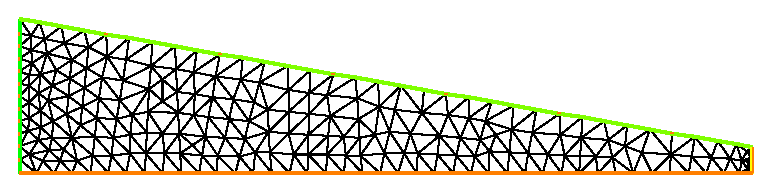
\includegraphics[width=15cm]{dTh}
\caption{The mesh of the domain $\Omega$}
\end{figure}

The free boundary problem is: 
 
Find $u$ and $\Omega$ such that:

 $$ \left\{\begin{array}{cl} 
 \displaystyle - \Delta u = 0  & \mbox{in } \Omega\\
 \displaystyle      u = y         &\mbox{on } \Gamma_b \\
 \displaystyle      {\partial u  \over \partial n} = 0   &\mbox{on } \Gamma_d \cup \Gamma_a \\
 \displaystyle    {\partial u  \over \partial n} = { q\over K} n_x  
	        \mbox{\ and \ } {u = y}  &\mbox{on\ } \Gamma_ f
\end{array}\right. $$


We use a fixe point method;
$\Omega^0 = \Omega$

in two step, fist we solve the classical following problem:
$$ \left\{\begin{array}{rll} 
 \displaystyle - \Delta u &= 0  & \mbox{in } \Omega^n\\
 \displaystyle      u &= y         &\mbox{on } \Gamma^n_b \\
 \displaystyle      {\partial u  \over \partial n} &= 0   &\mbox{on } \Gamma^n_d \cup \Gamma^n_a\\
 \displaystyle    u &= y        &\mbox{on\ } \Gamma^n_ f
\end{array}\right. $$

The varitional formulation is:

find $u$ on $V=H^1(\Omega^n)$, such than  $u=y$ on $\Gamma^n_b$ and $\Gamma^n_f$
$$
 \int_{\Omega^n}  \nabla u \nabla u' = 0,  \quad \forall u' \in V  \mbox{ with }  u' =0 \mbox{ on } 
\Gamma^n_b \cup \Gamma^n_f
$$


and secondly to construte a domain deformation $\mathcal{F}(x,y)=[x,y-v(x,y)]$ 

where $v$ is  solution of  the following problem: 

 $$ \left\{\begin{array}{rll} 
 \displaystyle - \Delta v &= 0  & \mbox{in } \Omega^n\\
 \displaystyle      v  &= 0         &\mbox{on } \Gamma^n_a \\
 \displaystyle      {\partial v \over \partial n} &= 0   &\mbox{on } \Gamma^n_b \cup \Gamma^n_d \\
 \displaystyle    {\partial v  \over \partial n}  &=  \displaystyle {\partial u  \over \partial n} - { q\over K} n_x  
	          &\mbox{on\ } \Gamma^n_ f
\end{array}\right. $$

The varitional formulation is:

find $v$ on $V$, such than  $v=0$ on $\Gamma^n_a$ 
$$
 \int_{\Omega^n}  \nabla v \nabla v' = \int_{\Gamma_f^n}  ({\partial u  \over \partial n} - { q\over K} n_x )v',  \quad \forall v' \in V  \mbox{ with }  v' =0 \mbox{ on } 
\Gamma^n_a 
$$

finaly the new domain 
$\Omega^{n+1} = \mathcal{F}(\Omega^n)$




The  \texttt{FreeFem++} :implementation is:

\bFF
@real q=0.02;      //flux entrant
@real K=0.5;           //permeabilit�

@fespace Vh(Th,P1);
@int j=0;

Vh u,v,uu,vv;

@problem Pu(u,uu,solver=CG) = @int2d(Th)( dx(u)*dx(uu)+dy(u)*dy(uu)) 
  + @on(b,f,u=y) ;

@problem Pv(v,vv,solver=CG) = @int2d(Th)( dx(v)*dx(vv)+dy(v)*dy(vv)) 
  +  @on (a, v=0) + @int1d(Th,f)(vv*((q/K)*N.y- (dx(u)*N.x+dy(u)*N.y))); 
  

@real errv=1;
@real erradap=0.001;
verbosity=1;
@while(errv>1e-6)
{
  j++;       
  Pu;
  Pv;
  @plot(Th,u,v ,wait=0);
  errv=int1d(Th,f)(v*v);
   real coef=1;

//  
  real mintcc = @checkmovemesh(Th,[x,y])/5.; 
  real mint = @checkmovemesh(Th,[x,y-v*coef]); 
  
  if (mint<mintcc ||  j%10==0) {  // mesh to bad => remeshing
    Th=@adaptmesh(Th,u,err=erradap ) ;
    mintcc = @checkmovemesh(Th,[x,y])/5.;     
  }
  
  @while (1) 
  {  	    
    real mint = @checkmovemesh(Th,[x,y-v*coef]); 
    
    if (mint>mintcc) break;
    
    cout << " min |T]  " << mint << endl;    
    coef /= 1.5;
  }
  
  Th=@movemesh(Th,[x,y-coef*v]); // calcul de la deformation 
  cout << "\n\n"<<j <<"------------ errv = " << errv << "\n\n";

}
@plot(Th,ps="d_Thf.eps");
@plot(u,wait=1,ps="d_u.eps");
\eFF

\begin{figure}[hbt]
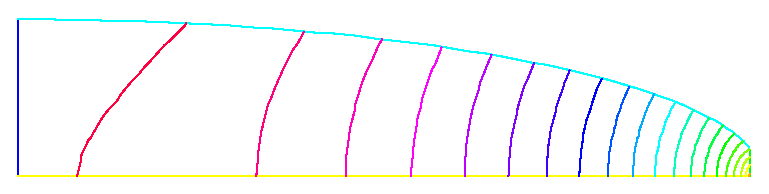
\includegraphics[width=15cm]{d_u}
\caption{The final solution on  the new  domain $\Omega^{72}$}
\end{figure}
\begin{figure}[hbt]
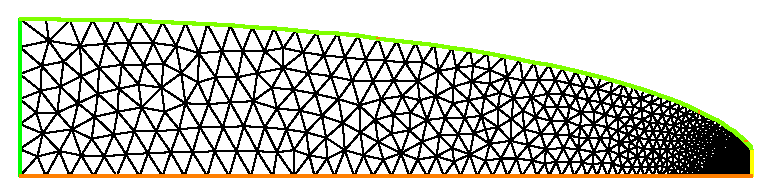
\includegraphics[width=15cm]{d_Thf}
\caption{The adapted mesh of the domain $\Omega^{72}$}
\end{figure}

\textBlack\subsection{nolinear-elas.edp}
\textBlack
The nonlinear elasticity  problem is find  the deplacement $(u_{1},u_{2})$  minimizing  $J$
$$ \min J(u_{1},u_{2}) = \int_{\Omega} f(F2) -  \int_{\Gamma_{p}} P_{a} \,  u_{2} $$
where  $F2(u_{1},u_{2}) =  A(E[u_{1},u_{2}],E[u_{1},u_{2}])$ and $A(X,Y)$ is bilinear sym. positive form with respect two matrix $X,Y$.
where $f$ is a given $\mathcal{C}^2$  function, and $E[u_{1},u_{2}] = (E_{ij})_{i=1,2,\,j=1,2}$ is the Green-Saint Venant deformation tensor defined  with: 
$$  E_{ij} = 0.5 ( \partial_i u_j + \partial_j u_i ) + \sum_k \partial_i u_k � \partial_j u_k  $$ 



The differential of $J$ is 
  $$ DJ(u_{1},u_{2})(v_{1},v_{2}) = \int 2 A(E[u_{1},u_{2}],DE[u_{1},u_{2}](v_{1},v_{2})) f'(F2(u_{1},u_{2}))) -  \int_{\Gamma_{p}} P_{a}  u_{2}  $$

denote $\mathbf{u}=u_{1},u_{2}$, $\mathbf{v}=v_{1},v_{2}$, $\mathbf{w}=(w_{1},w_{2})$ and  
the second order differential is
 {\begin{eqnarray*}
 D^2 J(\mathbf{u})((\mathbf{v}),(\mathbf{w}))  &= & A(E[\mathbf{u}],DE[\mathbf{u}](\mathbf{v})) A(E[\mathbf{u}],DE[\mathbf{u}](\mathbf{w})) f''(F2(\mathbf{u}))) \\
 & + &  A(DE[\mathbf{u}](\mathbf{v}),DE[\mathbf{u}](\mathbf{w})) f'(F2(\mathbf{u}))) \\
 &+&  A(DE[\mathbf{u}],D^{2}E[\mathbf{u}]((\mathbf{v}),(\mathbf{w}))) f'(F2(\mathbf{u}))) 
\end{eqnarray*}}
 where $DE$ and $D^{2}E$ are the first and second differential of $E$.
 
 \medskip
 

The Newton Method is

choose $ n=0$,and $u_O,v_O$ the initial displacement 
\begin{itemize}
\item loop: \par
\item  \hspace{1cm}    find $(du,dv)$ :  solution of 
$$ D^2J(u_n,v_n)((w,s),(du,dv)) =  DJ(u_n,v_n)(w,s) , \quad \forall w,s $$
\item  \hspace{1cm}      $un =un - du,\quad vn =vn - dv$ 
\item  \hspace{1cm}      until $(du,dv)$ small is enough
\end{itemize}

\color{black}The way to implement this algorithme in \freefempp is
use a macro tool to implement  $A$ and $F2$, $f$, $f'$,$f''$.

A macro\label{macro}\index{macro} is like is \texttt{ccp} preprocessor of \Cpp, but this begin by 
\texttt{macro} and the end of the macro definition is the begin of the comment $//$.
In this case the macro is very useful because the type of parameter can be change. 
And  it is easy to make automatic differentiation.

\bFF  
//  non linear elasticity model \hfilll
//   \hfilll
//  -------------------------------\hfilll
//  with huge utilisation of  macro\hfilll
// ---------------------------\hfilll
//   optimize version \hfilll
// ------------\hfilll
//  @problem is  find $(uu,vn)$  minimizing  $J$\hfilll
//  $ min J(un,vn) = @int f(F2) -  @int Pa * un $\hfilll
//   $ dJ(u,u,uu,vv) = @int dF2(u,v,uu,vv) df(F2(u,v))$ \hfilll
//   where $F2 =  (^t {E}  A {E} )$ , \hfilll
//   $E(U) =  1/2 (\nabla U + \nabla U^t + \nabla U^t  \nabla U) $ \hfilll
//         ($u_1$) \hfilll
//  with U=(   )\hfilll
//         ($u_2$)\hfilll
// so: \hfilll
// \hfilll$$ E_{ij} = 0.5 ( d_i u_j + d_j u_i ) + \sum_k d_i u_k * d_j*u_k  \leqno(1)$$ 
//  the 3 componantes of the Green Saint Venant deformation tensor: \hfilll
//  $E1(u1,u2) =    E_{11} $\hfilll
//  $E2(u1,u2) =    E_{12} = E_21 $\hfilll
//  $E3(u1,u2) =    E_{22}  $\textBlack\hfilll
\eFF
~
\bFF
// remark : we can parametrize E1,E2,E3 with:\hfilll
//  EE(da,db,a,b,u1,u2) \hfilll
//   where $da,db$ correspond to $d_i, d_j$ in (1)\hfilll
//   where  $a,b$  correspond to $u_i, u_j$ in (1)\hfilll
//   where $u1,u2$  correspond to $u_1, u_2$ in (1)\hfilll
//  ----------------------------------------------

//  first the linear part of EE linear elasticite\hfilll
// remark a macro end with a // comment \hfilll
@macro EEL(di,dj,ui,uj) ( (di(uj)+dj(ui))*0.5 )    // 11

// non linear par of EE (bilinear)  simple to differential \hfilll
@macro bEENL(di,dj,u1,u2,v1,v2) (di(u1)*dj(v1)*.5+di(u2)*dj(v2)*0.5) 
// 
@macro EENL(di,dj,u1,u2) bEENL(di,dj,u1,u2,u1,u2) // 
@macro dEENL(di,dj,u1,u2,du1,du2) ( bEENL(di,dj,du1,du2,u1,u2) 
                                  + bEENL(di,dj,u1,u2,du1,du2) )   
//   ------------ \hfilll
@macro EE(di,dj,ui,uj,u1,u2) (EEL(di,dj,u1,uj) + EENL(di,dj,u1,u2)) //
@macro dEE(di,dj,dui,duj,u1,u2,du1,du2) (EEL(di,dj,du1,duj) 
                                         + dEENL(di,dj,u1,u2,du1,du2)) //
@macro ddEE(di,dj,du1,du2,ddu1,ddu2) ( dEENL(di,dj,du1,du2,ddu1,ddu2)) 
//
// remark  : \hfilll
// $ dEE(di,dj,dui,duj,u1,u2,du1,du2)$  is "the formal differential of EE" \hfilll
// where $du1=\delta u1$ ,$du2=\delta u2$ \hfilll
// $ ddEE(di,dj,dui,duj,u1,u2,du1,du2)$  is "the formal differential of dEE" \hfilll
// where $ddu1=\delta^2 u1$ ,$ddu2=\delta^2 u2$ \hfilll
// --- \hfilll

//  the macro corresponding to the 3 componante of E \hfilll
@macro E1(u,v)  /*E11*/EE(dx,dx,u,u,u,v)  //
@macro E2(u,v)  /*E12*/EE(dx,dy,u,v,u,v)  //
@macro E3(u,v)  /*E22*/EE(dy,dy,v,v,u,v)  //

@macro dE1(u,v,uu,vv) /*dE11*/dEE(dx,dx,uu,uu,u,v,uu,vv) // 
@macro dE2(u,v,uu,vv) /*dE12*/dEE(dx,dy,uu,vv,u,v,uu,vv) //
@macro dE3(u,v,uu,vv) /*dE22*/dEE(dy,dy,vv,vv,u,v,uu,vv) //
@macro ddE1(u,v,uu,vv,uuu,vvv) /*ddE11*/ddEE(dx,dx,uu,vv,uuu,vvv) //
@macro ddE2(u,v,uu,vv,uuu,vvv) /*ddE12*/ddEE(dx,dy,uu,vv,uuu,vvv) //
@macro ddE3(u,v,uu,vv,uuu,vvv) /*ddE22*/ddEE(dy,dy,uu,vv,uuu,vvv) 
//
//  a formal bilinear term \hfilll
@macro PP(A,B,u,v) (A(u,v)*B(u,v)) 
// 
// a formal diff  bilinear term \hfilll
@macro dPP(A,B,dA,dB,u,v,uu,vv) (dA(u,v,uu,vv)*B(u,v) + A(u,v)*dB(u,v,uu,vv)) 
//
// a formal $diff^2$ bilinear term \hfilll
@macro ddPP(A,B,dA,dB,ddA,ddB,u,v,uu,vv,uuu,vvv) (
  dA(u,v,uu,vv)*dB(u,v,uuu,vvv) + dA(u,v,uuu,vvv)*dB(u,v,uu,vv) 
  +  ddA(u,v,uu,vv,uuu,vvv)*B(u,v) + A(u,v)*ddB(u,v,uu,vv,uuu,vvv) 
  ) //
// so the @matrix A is 6 coef \hfilll
//      
//     a11 a12 a13 \hfilll
//     a12 a22 a23 \hfilll
//     a13 a23 a33 \hfilll
@macro F2(u,v)  /* F2 */  (
     a11*PP(E1,E1,u,v)
  +  a22*PP(E2,E2,u,v)
  +  a33*PP(E3,E3,u,v)
  +  a13*PP(E1,E3,u,v)
  +  a13*PP(E3,E1,u,v)
  +  a12*PP(E1,E2,u,v)
  +  a12*PP(E2,E1,u,v)
  +  a23*PP(E2,E3,u,v)
  +  a23*PP(E3,E2,u,v)
)  // end macro F2

@macro dF2(u,v,uu,vv)  /* dF2 */  (
       a11*dPP(E1,E1,dE1,dE1,u,v,uu,vv)
     + a12*dPP(E1,E2,dE1,dE2,u,v,uu,vv)
     + a13*dPP(E1,E3,dE1,dE3,u,v,uu,vv)
     + a21*dPP(E2,E1,dE2,dE1,u,v,uu,vv)
     + a22*dPP(E2,E2,dE2,dE2,u,v,uu,vv)
     + a23*dPP(E2,E3,dE2,dE3,u,v,uu,vv)
     + a31*dPP(E3,E1,dE3,dE1,u,v,uu,vv)
     + a32*dPP(E3,E2,dE3,dE2,u,v,uu,vv)
     + a33*dPP(E3,E3,dE3,dE3,u,v,uu,vv)
) // end macro dF2 ($D F2$)

@macro ddF2(u,v,uu,vv,uuu,vvv)  /* ddF2 */  (
       a11*ddPP(E1,E1,dE1,dE1,ddE1,ddE1,u,v,uu,vv,uuu,vvv)
     + a12*ddPP(E1,E2,dE1,dE2,ddE1,ddE2,u,v,uu,vv,uuu,vvv)
     + a13*ddPP(E1,E3,dE1,dE3,ddE1,ddE3,u,v,uu,vv,uuu,vvv)
     + a21*ddPP(E2,E1,dE2,dE1,ddE2,ddE1,u,v,uu,vv,uuu,vvv)
     + a22*ddPP(E2,E2,dE2,dE2,ddE2,ddE2,u,v,uu,vv,uuu,vvv)
     + a23*ddPP(E2,E3,dE2,dE3,ddE2,ddE3,u,v,uu,vv,uuu,vvv)
     + a31*ddPP(E3,E1,dE3,dE1,ddE3,ddE1,u,v,uu,vv,uuu,vvv)
     + a32*ddPP(E3,E2,dE3,dE2,ddE3,ddE2,u,v,uu,vv,uuu,vvv)
     + a33*ddPP(E3,E3,dE3,dE3,ddE3,ddE3,u,v,uu,vv,uuu,vvv)
) // end macro ddF2  ($D^{2}  F2$)

//  differential of J: \hfilll

//  @for hyper elasticity @problem  \hfilll
//  ------------------------------ \hfilll

@macro f(u) (u) // end of macro  
@macro df(u) (1) // end of macro  $df=f'$
@macro ddf(u) (0) // end of macro $ddf=f''$

//  -- du caouchouc --- CF cours de Herve Le Dret. \hfilll
// ------------------------------- \hfilll
@real mu = 0.012e5; //  $kg/cm^2$
@real lambda =  0.4e5; //  $kg/cm^2$
//  \hfilll
//   $  \sigma = 2 \mu E + \lambda tr(E) Id $  \hfilll
//    \hfilll
//   ( a b )  \hfilll
//   ( b c )  \hfilll
//  \hfilll
//  tr*Id : (a,b,c) -> (a+c,0,a+c)  \hfilll
// so the associed @matrix is:  \hfilll
//   ( 1 0 1 )  \hfilll
//   ( 0 0 0 )  \hfilll
//   ( 1 0 1 )  \hfilll
// ------------------ the coef \hfilll
@real a11= 2*mu +  lambda  ;
@real a22= 2*mu ;
@real a33= 2*mu +   lambda ;
@real a12= 0 ;
@real a13= lambda ;
@real a23= 0 ;
//  symetric part
@real a21= a12 ;
@real a31= a13 ;
@real a32= a23 ;
@real Pa=1e2; //  a pressure of 100 Pa
// ----------------

@int n=30,m=10;
@mesh Th= square(n,m,[x,.3*y]); // label: 1 bottom, 2 right, 3 up, 4 left;
@int bottom=1, right=2,upper=3,left=4;

@plot(Th);
 
@fespace Wh(Th,P1dc);
@fespace Vh(Th,[P1,P1]);
@fespace Sh(Th,P1);

Wh e2,fe2,dfe2,ddfe2; // optimisation 
Wh ett,ezz,err,erz; // optimisation 

Vh [uu,vv], [w,s],[un,vn];
[un,vn]=[0,0];//  intialisation 
[uu,vv]=[0,0];

@varf vmass([uu,vv],[w,s],solver=CG) =  @int2d(Th)( uu*w + vv*s );
@matrix M=vmass(Vh,Vh);

@problem NonLin([uu,vv],[w,s],solver=LU)=
 @int2d(Th,qforder=1)( // $(D^2 J(un))$ part
               ddF2(un,vn,uu,vv,w,s)* dfe2 
	     + dF2(un,vn,uu,vv)*dF2(un,vn,w,s)*ddfe2        
	      )
   -@int2d(Th,<1)( // $(D J(un))$ part
           dF2(un,vn,w,s) * dfe2  )
   - @int1d(Th,3)(Pa*s) 
   + @on(right,left,uu=0,vv=0);
;
// Newton's method
// ---------------
Sh u1,v1;
@for (@int i=0;i<10;i++)
{
  @cout << "Loop " << i << @endl;
  e2 = F2(un,vn);
  dfe2 = df(e2) ;
  ddfe2 = ddf(e2);
  @cout << "  e2 max " <<e2[].max << " , min" << e2[].min << @endl;
  @cout << " de2 max "<< dfe2[].max << " , min" << dfe2[].min << @endl;
  @cout << "dde2 max "<< ddfe2[].max << " , min" << ddfe2[].min << @endl;
  NonLin; //  compute $[uu,vv] = (D^2 J(un))^{-1}(D J(un))$
  
  w[]   = M*uu[];
  @real res = sqrt(w[]' * uu[]); //  norme $ L^2 of [uu,vv]$
  u1 = uu;
  v1 = vv;
  @cout << " L^2 residual = " << res << @endl;
  @cout << " u1 min =" <<u1[].min << ", u1 max= " << u1[].max << @endl;
  @cout << " v1 min =" <<v1[].min << ", v2 max= " << v1[].max << @endl;
  @plot([uu,vv],wait=1,cmm=" uu, vv " );
  un[] -= uu[]; 
  @plot([un,vn],wait=1,cmm=" deplacement " );
  @if (res<1e-5) @break;
}

@plot([un,vn],wait=1);
@mesh th1 = @movemesh(Th, [x+un, y+vn]);
@plot(th1,wait=1); //  see figure \ref{fig nl-elas}
\eFF

\begin{figure}[hbt]
\begin{center}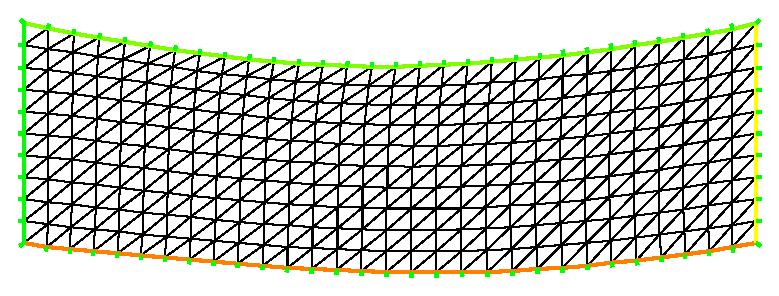
\includegraphics[width=16cm]{nl-elas}\end{center}
\caption{\label{fig nl-elas} The deformated domain}
\end{figure}



\section{Parallel version experimental}
A first test of parallisation of \texttt{FreeFem++} is make under mpi.
We add three word in the language:
\begin{description}
\itemtt[mpisize] The total number of  processes\index{mpisize}
\itemtt[mpirank]  the number of my current process in $\{0,..., mpisize-1\}$.\index{mpirank}
\itemtt [processor] a function to set the possessor to send or receive data 
\itemtt [broadcast] a function to broadcast from a processor to all other a data \index{broadcast}\index{processor}
\bFF
    processor(10) << a ; // send to the process 10 the data a;
    processor(10) >> a ; // receive from the process 10 the data a;

\eFF
\end{description}
\subsection{Schwarz in parallel}
If example is just the rewritting of example \texttt{schwarz-overlap} 
in section \ref{schwarz-overlap}.\index{schwarz}\index{broadcast}\index{processor}
\index{array!mesh}

How to use 
\bFF
[examples++-mpi] hecht%lamboot

LAM 6.5.9/MPI 2 C++/ROMIO - Indiana University


[examples++-mpi] hecht% mpirun -np 2 FreeFem++-mpi schwarz-c.edp
\eFF

\bFF
//  a new coding verion c,   methode de schwarz in parallele \hfilll
// with 2 proc. \hfilll
//  ------------------------------- \hfilll
// F.Hecht december 2003 \hfilll
// ---------------------------------- \hfilll
//  to test the broadcast instruction \hfilll
//  and array of mesh  \hfilll
//  add add the stop test \hfilll
//  --------------------------------- \hfilll

@if ( mpisize != 2 ) {
  @cout << " sorry number of processeur !=2 " << endl;
  exit(1);}
@verbosity=3;
@real pi=4*atan(1);
@int inside = 2;
@int outside = 1;
@border a(t=1,2){x=t;y=0;label=outside;};
@border b(t=0,1){x=2;y=t;label=outside;};
@border c(t=2,0){x=t ;y=1;label=outside;};
@border d(t=1,0){x = 1-t; y = t;label=inside;};
@border e(t=0, pi/2){ x= cos(t); y = sin(t);label=inside;};
@border e1(t=pi/2, 2*pi){ x= cos(t); y = sin(t);label=outside;}; 
@int n=4;
@mesh[int]  Th(mpisize);
@if (mpirank == 0) 
 Th[0] = buildmesh( a(5*n) + b(5*n) + c(10*n) + d(5*n));
@else
 Th[1] = buildmesh ( e(5*n) + e1(25*n) );

@broadcast(@processor(0),Th[0]);
@broadcast(@processor(1),Th[1]);

@fespace Vh(Th[mpirank],P1);
@fespace Vhother(Th[1-mpirank],P1);

Vh u=0,v;
Vhother U=0;
@int i=0;

@problem pb(u,v,init=i,solver=Cholesky) = 
    @int2d(Th[mpirank])( dx(u)*dx(v)+dy(u)*dy(v) )
  - @int2d(Th[mpirank])( v) 
  + @on(inside,u = U)  +  @on(outside,u= U ) ;

@for ( i=0 ;i< 20; i++) 
{ 
  @cout << mpirank << " looP " << i << endl;
   pb; 
   //  send u  to the other proc, receive in U
   @processor(1-mpirank) << u[];   @processor(1-mpirank) >> U[];
   @real err0,err1;
   err0 = int1d(Th[mpirank],inside)(square(U-u)) ;
   // send err0  to the other proc, receive in err1
   @processor(1-mpirank)<<err0;   @processor(1-mpirank)>>err1;
   @real err= sqrt(err0+err1);
   @cout <<" err = " << err << " err0 = " << err0 << ", err1 = " << err1 << endl;
   @if(err<1e-3) @break;
};
@if (mpirank==0)  
    @plot(u,U,ps="uU.eps");

\eFF



\section{Graphical User Interface} \label{GUI}

%There are two different graphical user interfaces available for
%\freefempp:

%\begin{itemize}
%\item 
\texttt{FreeFem++-cs} is part of the standard \freefempp
package. It runs on Linux, MacOS X and Windows.
%\item \texttt{FFedit} is available as a separate package. It runs on
%Linux and MacOS~X and requires tcl/tk to be installed.
%\end{itemize}

%\subsection{FreeFem++-cs}

``-cs'' stands for ``client/server''. The executable program named
\texttt{FreeFem++-cs} contains code for running a graphical user
interface client and a computational server. The server is
automatically started every time every time the user asks for a script
to be run. To run \texttt{FreeFem++-cs}, just type its name in,
optionally followed by a script name. It will open a window
corresponding to fig. \ref{fig:FreeFem++-cs}.

\begin{figure}[htbp]
\begin{center}
  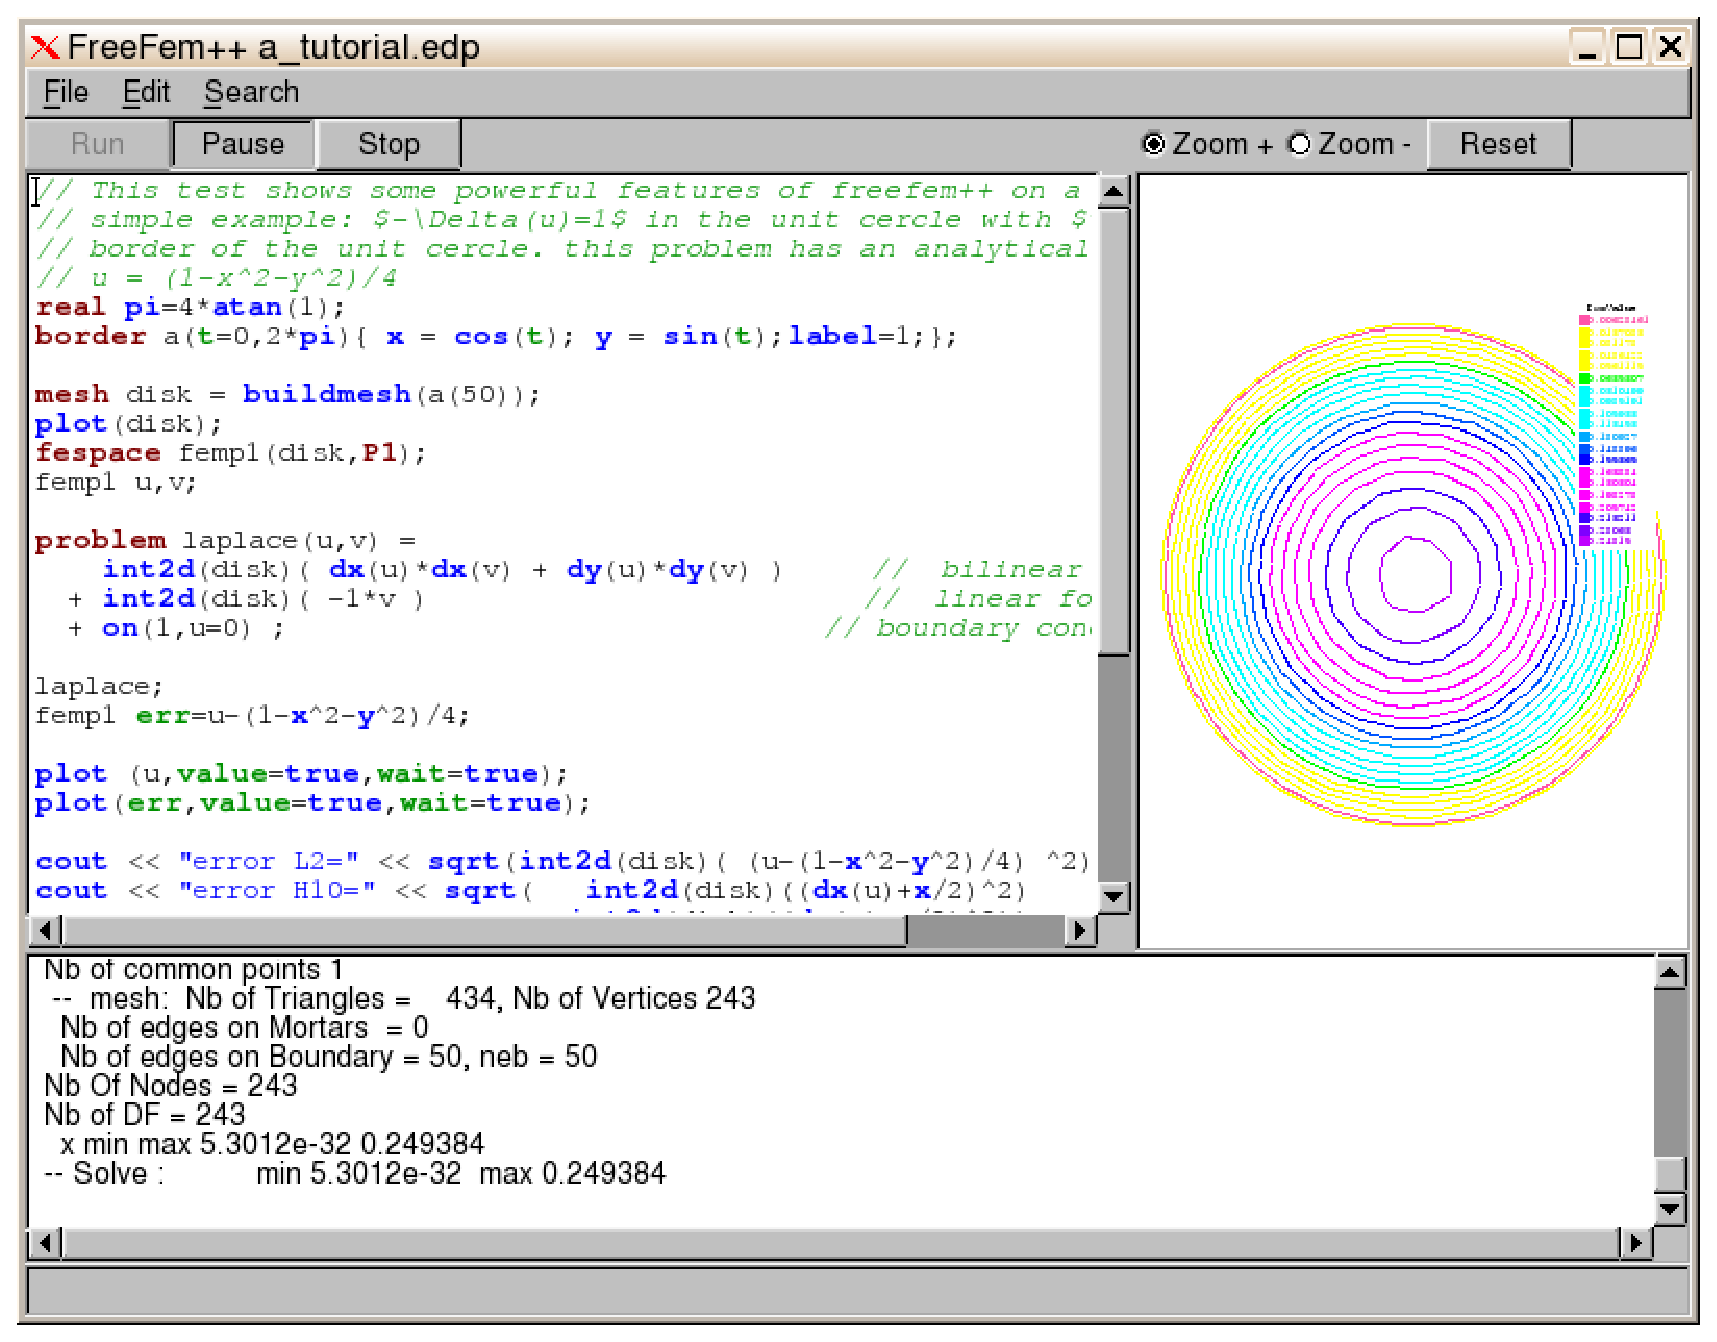
\includegraphics[height=10cm]{FreeFem++-cs}
\end{center}
  \caption{\texttt{FreeFem++-cs} main window}
  \label{fig:FreeFem++-cs} \index{label}
\end{figure}

\bigskip

The main characteristics of \texttt{FreeFem++-cs} are~:

\begin{itemize}
\item A main window composed of three panels~: editor with syntax
highlighting (right), \freefempp messages (bottom) and graphics
(left).
\item Panel sizes can be changed by dragging their borders with the
mouse. Any of the three panels can be made to fill the whole window.
\item The edited script can be run at any time by clicking on the
``Run'' button.
\item Dragging a \freefempp script file icon from a file manager into
the editor window makes \texttt{FreeFem++-cs} edit that script.
\item Graphics can be examined (e.g. zoomed) while \freefempp is
running.
\item A running \freefempp computation can be paused or stopped at any
time.
\end{itemize}

\bigskip

All commands should be self-explanatory. Here are just a few
useful hints~:

\begin{itemize}
\item There is no need to save a \freefempp script to run it. It is
  run exactly as displayed in the editor window, and the corresponding
  file is not touched.
\item The current directory is updated every time a script is loaded
  or saved. All \texttt{include} directives are therefore relative to
  the directory where the main script is located.
\item Specifying \texttt{wait=1} in a \texttt{plot} command is exactly
  equivalent to clicking on the ``Pause'' button when the plot is
  displayed.
\item In zoom mode, if your mouse has more than one button, a
  middle-click resets any zooming coefficient, and a right-click zooms
  in the opposite way of the left-click.
\end{itemize}

%\subsection{FFedit}

%FFedit runs on Linux and MacOSX.

%\subsubsection{Installation of Tcl and Tk}

%You have to install tcl8.4.6 and tk8.4.6 for the GUI to work.\\
%First go to http:\\
%//www.tcl.tk./software/tcltk/downloadnow84.tml \\
%and download :\\
%tcl8.4.6-src.tar.gz and tk8.4.6-src.tar.gz\\
%Then do :\\
%tar zxvf tcl8.4.6-src.tar.gz\\
%tar zxvf tk8.4.6-src.tar.gz\\
%It creates two directories : tcl8.4.6 and tk8.4.6\\
%Now do : \\
%cd tcl8.4.6\\
%cd unix (if your OS is Linux or MacOSX)\\
%./configure\\
%make\\
%make install\\
%\\
%then \\
%cd tk8.4.6\\
%cd unix\\
%./configure\\
%make\\
%make install\\
%\\
%At the end of installation, you have to find where is your binary ``wish'' or ``wish84'' or ``wish8.4'' by typing :\\
%-$>$ which wish (or wish84 or wish8.4)\\
%If wish84 does exist it is all. If not, you have to go in the directory where is ``wish'' or ``wish8.4'' (for example /usr/bin/)\\
%and then create a link :\\
%-$>$ ln -s wish wish84\\
%or\\
%-$>$ ln -s wish8.4 wish84\\

%\subsubsection{Description}

%The Graphic User Interface is in the directory called FFedit.
%You can run it by typing ./FFedit.tcl\\
%\
%The Graphic User Interface shows a text window with buttons on the left and right side, a horizontal menu bar above and an entry below where you can see the path of the script when it is opened or where you can type the path of a script to run it.\\
%\\
%This is the description of the different functions of the GUI :\\
%\\
%*New : you can access it by the button ``New'' on the right side or by selecting it in the menu File on the horizontal bar.\
%It deletes the current script and enables you to type a new script.\\
%\\
%*Open : you can access it by the button ``Open'' on the right side or by selecting it in the menu File or by typing simultaneously ctrl+o on the keyboard.\
%It enables you to select a script which has been saved. This script is then opened in the text window. Then, you can modify it, save the changes, save under another name or run it.\\
%\\
%*Save : you can access it by the button ``Save'' on the right side or by selecting it in the menu File or by typing simultaneously ctrl+s on the keyboard.\
%It enables you to save the changes of a script.\\
%\\
%*Save as : you can access it by the button ``Save As'' on the right side or by selecting it in the menu File.\\
%It enables you to locate where you want to save your script and to choose your the name of your script.\\
%\\
%*Run : you can access it by the button ``Run'' on the right side or by selecting it in the menu File or by typing simultaneously ctrl+r on the keyboard.\\
%It enables you to run the current script.\\
%Warning: when you run by typing ctrl+r, the cursor must be in the text window.\\
%\\
%*Print : you can access it by the button ``Print'' on the right side or by selecting it in the menu File or by typing simultaneously ctrl+p on the keyboard.\\
%It enables you to print your script. You have to choose the name of the printer.\\
%\\
%*Help (under construction) : you can access it by the button ``Help'' on the left side. When an example is opened, it shows you a documentation about this example.\\
%Warning : The bottom of each page is not accessible, you have to print to see the entire document.\\
%\\
%*Example : you can access it by the button ``Ex'' on the left side.\
%It runs a little example.\\
%\\
%*Read Mesh : you can access it by the button ``R.M'' on the left side.\
%It enables you to read a mesh which has been saved. It adds the command in your script so that you can use it in your script.\\
%\\
%*Polygonal Border : you can access it by the button ``P.B'' on the left side.\\
%It enables you to build a polygonal border.\\
%When you click on this button, a new window is opened : you have to click on the button ``Border'' then it asks you how many borders you want. When you enter a number and click on ``OK'' the exact number of couple of entries enable you to enter the coordinates of the vertices. And then you have to enter the number of points on each border. The border number 1 is the segment between the vertex number 1 and the vertex number 2 ...etc...\\
%You must turn in the opposite sens of needles of a watch.\\
%When you have finished, you have to click on the button ``Build''. It builds the domain with polygonal border and shows the result.\\
%Then you can save the result by clicking on the button ``S.Mesh''. Choose the extension .msh for the name.\\
%\\
%*Navier Stokes : you can access it by the button ``N.S'' on the left side.\\
%A new window is opened. You have to build your polygonal domain by clicking on the button ``Border'' it works like the Polygonal Border function.\\
%You can save by clicking on the button ``S.Mesh''. Choose the extension .msh for the name.\\
%Then you have to choose the Limits Condition by clicking on the buton ``L.C''.\\
%First choose between ``Free'' or ``Imposed', then click on the button ``Validate'' and enter the expression of Imposed condition. You have to enter the tangential and the normal component of the velocity. Then click on ``Validate'' again.\\
%The expression of the limit condition can be a number but a mathematical expression as well.\\
%\\
%*emc2 : you can access it by the button ``emc2''. It runs emc2 the mesh building software \\
%(http://www-rocq1.inria.fr/gamma/cdrom/\\
%www/emc2/fra.htm)\\
%\\
%*Set up : you can access it by the button ``set up''. It is the first thing you have to do when you use FFedit for the first time.\\
%When you click on this button, a new window is opened, with two entries where you have to enter the path of the binary of FreeFem++ (where you compiled or installed) and the path of the scripts (programs written with FreeFem++) for instance the examples provided in FreeFem++.\\
%\\
%*Undo : you can access it by selecting in the menu Edit or by typing simultaneously ctrl+z. It is an unlimited undo function.\\
%\\
%*Redo : you can access it by selecting in the menu Edit or by typing simultaneously ctrl+e. It is an unlimited redo function.\\
%\\
%*Cut : you can access it by selecting in the menu Edit or by typing simultaneously ctrl+x on the keyboard.\\
%\\
%*Copy : you can access it by selecting in the menu Edit or by typing simultaneously ctrl+c on the keyboard.\\
%\\
%*Paste : you can access it by selectiog in the menu Edit or by typing simultaneously ctrl+y on the keyboard.\\
%\\
%*Delete : you can access it by selecting in the Edit menu. It is a Delete function.\\
%\\
%*Select all : you can access it by selecting in the Edit menu or by typing simultaneously ctrl+l. This function select all the text you have written, so you can delete, cut copy paste etc...\\
%\\
%*Background : you can access it by selecting in the menu Color. You can then choose the color of the background.\\
%\\
%*Foreground : you can access it by selecting in the menu Color. You can then choose the color of the foreground.\\
%\\
%*Syntax Color : you can access it by selecting in the menu Color. It enables the syntax coloring of your FreeFem++ script.\\
%\\
%*Family : you can access it by selecting in the menu Font. You can then choose the style of your characters.\\
%\\
%*Size : you can access it by selecting in the menu Font. You can then choose the size of your characters.\\
%\\
%*Find : you can access it by selecting in the menu Search. It enables you to find a word in the whole text. (This function doesn't work yet.)\\
%\\
%*Find next : you can access it by slecting in the menu Search. It enables you to find a word from the position of the cursor.(This function doesn't work yet.)\\
%\\
%*Replace : you can access it by selecting in the menu Search. It enables you to replace a word by another in the whole text.\\

%\subsubsection{Cygwin version}

%This version is for Windows.\\

%\subsubsection{Installation of Cygwin}
%First you have to go to the site:\\
%http://www.cygwin.com \\
%Click on ``Install or Update now''\\
%A window appears. \\
%Click on ``Open'' then ``Next'' and then choose ``Install from Internet''\\
%Click on ``Next'' twice and choose ``Direct Connection''.\\
%Then choose one of the download sites.\\
%For instance : ftp://ftp-stud.fht-esslingen.de\\
%Then choose in each category the options to install. \\
%(click on the symbol + for each, you can then see the options appear)\\
%\\
%Here are the required options for FreeFem++ and TCL TK to work :\\
%+ all options of ``Devel'' (it includes gcc ...etc...)\\
%+ all options of ``Graphics'' (specially ``Gnuplot'' to be able \\
%to see the results of FreeFem++ on a graphic)\\
%+ all options of X11 and XFree86 \\
%\\
%You can install ``Xemacs'' and others editors in the category ``Editors''.\\
%\\
%Then click on ``Next'' and wait that Cygwin is installed.\\
%Then an ic�ne appears on yours Desktop.\\
%Click on it and the Cygwin window is opened. It is like an Unix terminal.\\
%\\
%To work on a terminal X type : \\
%-$>$ startX\\
%You will have to work on a terminal X to have Gnuplot and visualize \\
%the results of FreeFem++ scripts)\\
%\\
%Now you have to compile and install FreeFem++.\\
%\\
%\subsubsection{Compilation and Installation of FreeFem++ under Cygwin}
%go to the site :\\
%http://www.freefem.org\\
%click on FreeFem++\\
%and download FreeFem++ (the version when I wrote this is 1.38)\\
%Choose to download in your cygwin/home/you directory.\\
%\\
%Then on your terminal Cygwin type :\\
%-$>$ tar zxvf freefem++.tgz\\
%to uncompress this file.\\
%\\
%Go into FreeFem++v1.38 directory by typing:\\
%-$>$ cd FreeFem++v1.38\\
%\\
%Now you have to compile FreeFem++.\\
%type:\\
%-$>$ make all HOSTTYPE=i-386\\
%to compile FreeFem++\\
%If there is an error : ``... -ldl : no such file or directory''\\
%Then you have to modify the Makefile-i386 which is in the directory src:\\
%-$>$ cd src \\
%Edit it (with xemacs for example):\\
%-$>$ xemacs Makefile-i386\\
%at line 1 : replace ``LIBLOCAL = -ldl'' by ``\#LIBLOCAL = -ldl''\\
%It will comment this line because -ldl is not on your machine.\\
%Then return to the main directory\\
%-$>$ cd\\
%and type:\\
%-$>$ make all HOSTTYPE=i-386\\
%\\
%At the end of compilation, a directory called ``c-i386'' is created.\\
%In this directory you can find the binary FreeFem++.\\
%\\
%You can now run an example:\\
%First open an X terminal:\\
%-$>$ startX\\
%In this terminal go in to FreeFem++v1.38:\\
%-$>$ cd FreeFem++v1.38\\
%and type:\\
%-$>$c-i386/FreeFem++ examples++-tutorial/adapt.edp\\
%You can then see the gnuplot window with the graphical results.\\
%\\

%\subsubsection{Compilation and Installation of tcl8.4.0 and  tk8.4.0 under Cygwin}
%Now if you want to use the Graphical User Interface of FreeFem++\\
%(called FFedit)\\
%you have to install the language TCL TK in which FFedit has been written.\\
%The version which works under cygwin is tcl8.4.0 and tk8.4.0\\
%The latest version when I wrote this is tcl8.4.6 and tk8.4.6\\
%\\
%DON'T USE IT \\
%\\
%It works under Linux and MacOsX but not under Cygwin.\\
%\\
%You have to download tcl8.4.0 and tk8.4.0 :\\
%For instance, go to Google.fr and type download tcl tk 8.4.0\\
%And choose the ``Sourceforge.net: Project Filelist''.\\
%Choose :\\
%tcl8.4.0-src.tar.gz and tk8.4.0-src.tar.gz\\
%When the download is finished you have to uncompress these directories:\\
%-$>$ tar zxvf tcl8.4.0-src.tar.gz\\
%-$>$ tar zxvf tk8.4.0-src.tar.gz\\
%\\
%\\
%tcl8.4.0 and tk8.4.0 will work under Cygwin only if you apply \\
%a patch on both:\\
%These patches are on the site:\\
%http://www.xraylith.wisc.edu/~khan/software/tcl\\
%Choose ``Tcl/Tk8.4.0 for Cygwin\\
%Click on ``very preliminary Cygwin ports of Tcl/Tk8.4.0\\
%You are then on the site ftp\\
%Follow the instructions of the README or follow these instructions:\\
%\\
%1) Run :\\
%-$>$ xemacs tcl-8.4.0-cygwin.diff\\
%By doing this, you create a new file called ``tcl-8.4.0-cygwin.diff''\\
%on the site ftp click on ``tcl-8.4.0-cygwin.diff''\\
%Do a Copy/Paste of the contain into your xemacs window and save it.\\
%\\
%2) Do the same with ``tk-8.4.0-cygwin.diff''\\
%\\
%Now you have to apply the patch in tcl8.4.0 and tk8.4.0\\
%The two previous patch files (.diff) must be respectively \\
%in tcl8.4.0 and tk8.4.0 directories.\\
%-$>$ cp tcl-8.4.0-cygwin.diff tcl8.4.0\\
%-$>$ cp tcl-8.4.0-cygwin.diff tk8.4.0\\
%(If the two files are one level under tcl8.4.0 and tk8.4.0)\\
%\\
%Now apply the patches:\\
%type:\\
%\\
%-$>$ cd tcl8.4.0\\
%-$>$ patch -p0 -s $<$ tcl-8.4.0-cygwin.diff\\
%\\
%-$>$ cd
%\\
%-$>$ cd tk8.4.0\\
%-$>$ patch -p0 -s $<$ tk-8.4.0-cygwin.diff\\
%\\
%Now you can compile and install TCL TK under Cygwin:\\
%\\

%
%* compilation and installation of tcl8.4.0\\
%\\
%Go in to the directory tcl8.4.0/win\\
%-$>$ cd tcl8.4.0\\
%-$>$ cd win\\
%Then type :\\
%-$>$ ./configure\\
%The two steps remaining are make and make install\\
%type\\
%-$>$ make\\
%The compilation starts, when finished install by typing:\\
%-$>$ make install\\
%\\
%When finished try to see if it works by typing:\\
%-$>$ tclsh84\\
%if ok quit by typing ctrl-c\\

%*Compilation and installation of tk8.4.0\\
%\\
%Go in to the directory tk8.4.0/win\\
%-$>$ cd tk8.4.0\\
%-$>$ cd win\\
%Then type :\\
%-$>$ ./configure\\
%The two steps remaining are make and make install\\
%type\\
%-$>$ make\\
%The compilation starts, if you have errors like :\\
%\\
%windres -o tk.res.o --include ``C:/cygwin/home/ly/tk8.4.0/generic'' \\
%--include ``C Option-I is deprecated for setting the input format,\\
% please use -J instead''\\
%windres : can't open icon file 'tk.ico' : no such file or directory\\
%\\
%This file 'tk.ico' is in fact in the directory win/rc\\
%You have to copy it in the directory 'generic':\\
%Be in tk8.4.0\\
%type :\\
%-$>$ cp win/rc/tk.ico generic/\\
%\\
%If you compile again you will see that there is the same \\
%errors with the files:\\
%``buttons.bmp'' ``cursor00.cur'' ``cursor02.cur'' ...etc... \\
%``wish.exe.manifest'' and ``wish.ico''\\
%\\
%Do the same for these files.\\
%For the cursor*.cur files do once the command:\\
%-$>$ cp win/rc/cursor*.cur generic/\\
%\\
%when finished install by typing:\\
%-$>$ make install\\
%\\
%When finished try to see if it works by typing:\\
%-$>$ wish84\\
%if ok quit by typing ctrl-c\\

%\subsubsection{Use}
%Now everything is ok to use FFedit and FreeFem++ under Windows by Cygwin.\\
%WARNING: if you work on the Cygwin terminal you will not be able \\
%to see the graphical results of FreeFem++.\\
%\\
%You have to run an X terminal and run FFedit under this X terminal:\\
%\\
%To run an X terminal under cygwin type on your Cygwin terminal:\\
%-$>$ startX\\
%\\
%An X terminal runs:\\
%Under this terminal:\\
%type\\
%-$>$ cd FFedit\\
%-$>$ ./FFedit.tcl\\



\section{ Mesh Files}
 \def\Chars#1{{\tt (C*)}  #1}
 \def\Char#1{{\tt (C)}  #1}
 \def\Int#1{ {\tt(I)} #1}
 \def\Real#1{{\tt(R)} #1}
 \def\Bool#1{{\tt(B)} #1}
 \def\Vertex#1{{{\tt @@Vertex}#1}}
 \def\Edge#1{{{\tt @@Edge}#1}}
 \def\Triangle#1{{{\tt @@Tria}#1}}
 \def\Quadrangle#1{{{\tt @@Quad}#1}}
 \def\Tetrahedron#1{{{\tt @@Tetra}#1}}
 \def\Hexahedron#1{{{\tt @@Hexa}#1}}
 \def\Pentahedron#1{{{\tt @@Penta}#1}}
 \def\Loop#1#2{{\bf\Large(}\,#1\,{\bf\Large{,\,\,}}\,#2\,{\bf\Large)}}
 \def\requis{\hfill {\it  requis}}
 \def\facultatif{\quad\quad facultatif}
 \def\need#1{\hfill{\it  requiert le champ\,:\,#1}}

\subsection{File mesh data structure}
\index{file!data base}\index{file!bamg}
The mesh data structure, output of a mesh generation algorithm, 
refers to the geometric data structure and in some case to another
mesh data structure.

In this case, the fields are

\small
\begin{itemize}
\item {\tt MeshVersionFormatted 0}
\end{itemize}
\normalsize

\small
\begin{itemize}
\item {\tt Dimension} 
  \Int{dim} 

\item {\tt Vertices} 
  \Int{NbOfVertices}\\
  \Loop{\,\,\Loop{\Real{x$_i^j$}}{j=1,dim}\,\,,\,\Int{$Ref \phi_i^v$}}{i=1\,,\,NbOfVertices}

\item {\tt Edges} 
  \Int{NbOfEdges} \\
  \Loop{\Vertex{$^1_i$}\,,\,\Vertex{$^2_i$}\,,\,\Int{$Ref \phi_i^e$}}{i=1\,,\,NbOfEdges}

\item {\tt Triangles} 
  \Int{NbOfTriangles} \\
    \Loop{\Loop{\Vertex{$_i^j$}}{j=1,3}\,,\,\Int{$Ref \phi_i^t$} }{ i=1\,,\,NbOfTriangles}

\item {\tt Quadrilaterals} 
  \Int{NbOfQuadrilaterals} \\
    \Loop{\Loop{\Vertex{$_i^j$}}{j=1,4}\,,\,\Int{$Ref \phi_i^t$} }{ i=1\,,\,NbOfQuadrilaterals}

\item {\tt Geometry} \\
\Chars{FileNameOfGeometricSupport} \\

\begin{itemize}
\item {\tt VertexOnGeometricVertex} \\
   \Int{NbOfVertexOnGeometricVertex}\\
\Loop{\Vertex{$_i$}\,,\,\Vertex{$_i^{geo}$}}{i=1,NbOfVertexOnGeometricVertex}

\item {\tt EdgeOnGeometricEdge} \\
   \Int{NbOfEdgeOnGeometricEdge}\\
\Loop{\Edge{$_i$}\,,\,\Edge{$_i^{geo}$}}{i=1,NbOfEdgeOnGeometricEdge}
\end{itemize}

\item {\tt CrackedEdges} 
  \Int{NbOfCrackedEdges}\\
  \Loop{\Edge{$_i^1$}\,,\,\Edge{$_i^2$}}{i=1\,,\,{NbOfCrackedEdges}}

\end{itemize}
\normalsize

When the current mesh refers to a previous mesh, we have in addition

\small
\begin{itemize}
\item {\tt MeshSupportOfVertices} \\
\Chars{FileNameOfMeshSupport} \\
\begin{itemize}

\item {\tt VertexOnSupportVertex} \\
   \Int{NbOfVertexOnSupportVertex}\\
\Loop{\Vertex{$_i$}\,,\,\Vertex{$_i^{supp}$}}{i=1,NbOfVertexOnSupportVertex}

\item {\tt VertexOnSupportEdge} \\
   \Int{NbOfVertexOnSupportEdge}\\
\Loop{\Vertex{$_i$}\,,\,\Edge{$_i^{supp}$}\,,\,  \mbox{\Real{$u_i^{supp}$}}  }{i=1,NbOfVertexOnSupportEdge}

\item {\tt VertexOnSupportTriangle} \\
   \Int{NbOfVertexOnSupportTriangle}\\
\Loop{\Vertex{$_i$}\,,\,\Triangle{$_i^{supp}$}\,,\,
  \mbox{\Real{$u_i^{supp}$}}\,,\,  \mbox{\Real{$v_i^{supp}$}}  }
{\\ \hbox to 3cm {} i=1\,,\,{NbOfVertexOnSupportTriangle}}


\item {\tt VertexOnSupportQuadrilaterals} \\
   \Int{NbOfVertexOnSupportQuadrilaterals}\\
\Loop{\Vertex{$_i$}\,,\,\Quadrangle{$_i^{supp}$}\,,\,
  \mbox{\Real{$u_i^{supp}$}}\,,\,  \mbox{\Real{$v_i^{supp}$}}  }
{\\ \hbox to 3cm {} i=1\,,\,{NbOfVertexOnSupportQuadrilaterals}}


\end{itemize}

\end{itemize}
\normalsize



\subsection {bb File type for Store Solutions}
The file is formatted such that:
{\tt \obeylines
   2 nbsol nbv 2 
  $\left(\left(\mathtt{U}_{ij}, \quad \forall i \in \{1,...,\mathtt{nbsol}\}\right), \quad \forall j \in \{1,...,\mathtt{nbv}\}\right)$
 } 

where 
\begin{itemize}
\item {\tt  nbsol} is a integer equal to  the number of solutions.
\item  {\tt nbv} is  a integer equal to the number of vertex .
\item  {\tt U$_{ij}$} is a real equal the value of the $i$ solution at vertex $j$
on the associated mesh background if read file, generated if write file.
\end{itemize}
 
\subsection {BB File Type for Store Solutions}
The file is formatted such that:
{\tt \obeylines
  $ \mathtt{ \quad 2 \quad n \quad typesol^1 \quad ... \quad typesol^n \quad  nbv \quad 2}  $
  $\left(\left(\left( \mathtt{U}_{ij}^k, \quad \forall i \in \{1,...,\mathtt{typesol}^k\}\right), %
\quad \forall k \in \{1,...\mathtt{n}\}\right) %
 \quad \forall j \in \{1,...,\mathtt{nbv}\}\right)$
 } 

where 
\begin{itemize}
\item {\tt  n} is a integer equal to  the number of solutions 
\item $\mathtt{  typesol^k}$, type of the solution  number $ k$, is
  \begin{itemize}
   \item $\mathtt{typesol^k = 1}$ the solution {\tt k} is scalare  (1  value per vertex)
   \item $\mathtt{typesol^k = 2}$ the solution {\tt k} is vectorial  (2 values per unknown)
   \item $\mathtt{typesol^k = 3}$ the solution {\tt k} is a  $2� 2$ symmetric matrix  (3 values per vertex)
   \item $\mathtt{typesol^k = 4}$ the solution  {\tt k} is a  $2� 2$ matrix  (4 values per vertex)
   \end{itemize}

\item  {\tt nbv} is  a integer equal to the number of vertices
\item  {\tt U$_{ij}^k$} is a real equal the value of the component  $i$ of the solution  $k$ at vertex $j$
on the associated mesh background if read file, generated if write file.
\end{itemize}


\subsection{Metric File}
 A metric file can be of two types, isotropic or anisotropic.
\label{Metric file}

the isotrope file is such that  
{\tt \obeylines
   nbv  1 
   h$_i \quad \forall i \in \{1,...,\mathtt{nbv}\}$
}


where
\begin{itemize}
\item {\tt  nbv} is  a integer equal to the number of vertices.
\item   {\tt h$_i$} is the wanted mesh size near the vertex $i$ on background mesh,
the metric is $\mathcal{M}_i=h_i^{-2} Id$, where $ Id $ is the identity matrix.
\end{itemize}

The metric anisotrope
{\tt \obeylines
   nbv  3 
   a11$_i$,a21$_i$,a22$_i \quad \forall i \in \{1,...,\mathtt{nbv}\}$
}


where
\begin{itemize}
\item   {\tt nbv} is  a integer equal to the number of vertices,
\item  a11$_i$, a12$_i$, a22$_i$ is metric 
$\mathcal{M}_i = \left(\begin{smallmatrix} a11_i & a12_i \\ a12_i & a22_i \end{smallmatrix}\right)$ which define the wanted mesh size 
in a vicinity of  the vertex $i$
such that $h$ in direction $u \in \R^2$ is equal to $ |u|/\sqrt{u\cdot\mathcal{M}_i\, u}$ , where $\cdot$ is the dot product
in $\R^2$, and $|\cdot|$ is the classical norm.

\end{itemize}

\subsection{List of  AM\_FMT, AMDBA Meshes}
 \index{file!am}\index{file!am\_fmt}\index{file!amdba}
 The mesh is only composed of triangles and can be defined with the help of
the following two integers and four arrays:

  \begin{ttlist}
  \item [nbt] is the number of triangles.
  \item [nbv] is the number of vertices.
  
  \item [nu(1:3,1:nbt)] is an integer array giving the three vertex numbers
  
counterclockwise for each triangle.
 
  \item [c(1:2,nbv)]    is a real array giving the two coordinates of each vertex.
  \item [refs(nbv)]     is an integer array giving the reference numbers of the
vertices. 
  \item [reft(nbv)]     is an integer array giving the reference numbers of the 
triangles.
  \end{ttlist}

\paragraph{AM\_FMT Files}\label{AMFMT}
\index{file!am\_fmt}
In fortran the  {\tt am\_fmt}  files are read as follows:

\begin{verbatim}
     open(1,file='xxx.am_fmt',form='formatted',status='old')
       read (1,*) nbv,nbt
       read (1,*)  ((nu(i,j),i=1,3),j=1,nbt)
       read (1,*)  ((c(i,j),i=1,2),j=1,nbv)
       read (1,*)  ( reft(i),i=1,nbt)
       read (1,*)  ( refs(i),i=1,nbv)
     close(1)
\end{verbatim}

\paragraph{AM Files}\label{AM}
\index{file!am}
In fortran the  {\tt am}  files are read as follows:

\begin{verbatim}
     open(1,file='xxx.am',form='unformatted',status='old')
       read (1,*) nbv,nbt
       read (1)  ((nu(i,j),i=1,3),j=1,nbt),
     &   ((c(i,j),i=1,2),j=1,nbv),
     &   ( reft(i),i=1,nbt),
     &   ( refs(i),i=1,nbv)
     close(1)
\end{verbatim}
\paragraph{AMDBA Files}\label{AMDBA}
\index{file!amdba}
In fortran the  {\tt amdba}  files are read as follows:
\begin{verbatim}
     open(1,file='xxx.amdba',form='formatted',status='old')
       read (1,*) nbv,nbt
       read (1,*) (k,(c(i,k),i=1,2),refs(k),j=1,nbv)
       read (1,*) (k,(nu(i,k),i=1,3),reft(k),j=1,nbt)
     close(1)
\end{verbatim}
\paragraph{msh Files}\label{MSH}
\index{file!msh}
First, we add the notions of boundary edges
  \begin{ttlist}
  \item [nbbe] is the number of boundary edge.
  \item [nube(1:2,1:nbbe)] is an integer array giving the two vertex numbers
  \item [refbe(1:nbbe)] is an integer array giving the two vertex numbers
  \end{ttlist} 
In fortran the  {\tt msh}  files are read as follows:
\begin{verbatim}
     open(1,file='xxx.msh',form='formatted',status='old')
       read (1,*) nbv,nbt,nbbe
       read (1,*) ((c(i,k),i=1,2),refs(k),j=1,nbv)
       read (1,*) ((nu(i,k),i=1,3),reft(k),j=1,nbt)
       read (1,*) ((ne(i,k),i=1,2), refbe(k),j=1,nbbe)
     close(1)
\end{verbatim}
\paragraph{ftq Files}\label{FTQ}
\index{file!ftq}
In fortran the  {\tt ftq}  files are read as follows:
\begin{verbatim}
     open(1,file='xxx.ftq',form='formatted',status='old')
      read (1,*) nbv,nbe,nbt,nbq
      read (1,*) (k(j),(nu(i,j),i=1,k(j)),reft(j),j=1,nbe)
      read (1,*) ((c(i,k),i=1,2),refs(k),j=1,nbv)
     close(1)
\end{verbatim}
where   if {\tt  k(j) = 3} then the element $j$  is  a triangle and if {\tt k = 4}
the the element $j$   is a quadrilateral.

\section{Addition of a  new finite element}
\label{AddnewFE}
\subsection{Some notations}
\def\Fb#1{\boldsymbol{\omega}^{K}_{#1}}
\def\fbi{\mathbf{\omega}^{K}_{ij}}


For a function $\boldsymbol{f}$ taking value in $\R^{N},\,
N=1,2,\cdots$, we define the finite element approximation $\Pi_h
\boldsymbol{f}$ of $\boldsymbol{f}$. Let us denote the number of the
degrees of freedom of the finite element by $NbDoF$. Then the $i$-th
base  $\boldsymbol{\omega}^{K}_{i}$ ($i=0,\cdots,NbDoF-1$) of the
finite element space has the $j$-th component
$\mathbf{\omega}^{K}_{ij}$ for $j=0,\cdots,N-1$.

The operator  $\Pi_{h}$ is called the interpolator of the finite element.
We have the identity $\boldsymbol{\omega}^{K}_{i} =  \Pi_{h} \boldsymbol{\omega}^{K}_{i} $.

Formally, the interpolator $\Pi_{h}$ is constructed by the following formula:
\begin{equation}
\label{eq-interpo}
\Pi_{h} \boldsymbol{f} = \sum_{k=0}^{\mathtt{kPi}-1} \alpha_k \boldsymbol{f}_{j_{k}}(P_{p_{k}}) \boldsymbol{\omega}^{K}_{i_{k}}
\end{equation}
where $P_{p}$ is a set of $npPi$ points,

%\begin{remark}
In the formula (\ref{eq-interpo}), the list $ p_{k},\, j_{k},\, i_{k}$ depend just on  the type of finite element (not on the element), but the coefficient  $\alpha_{k}$ can be depending on the element.
%\end{remark}

\medskip
%\begin{example}
 Example 1: with the classical scalar  Lagrange finite element, we have $\mathtt{kPi}=\mathtt{npPi}=\mathtt{NbOfNode}$ and
\begin{itemize}
\item $P_{p}$ is the point of the nodal points
\item  the $\alpha_k=1$, because we take the value  of the function at the point $P_{k}$
\item $p_{k}=k$ ,  $j_{k}=k$ because we have one node per  function.
\item $j_{k}=0$ because $N=1$
\end{itemize}
%\end{example}

%\begin{example}
 Example 2: The Raviart-Thomas finite element:
\begin{equation}
         RT0_{h} = \{ \mathbf{v} \in H(div) / \forall K \in
         \mathcal{T}_{h} \quad  \mathbf{v}_{|K}(x,y) =
         \vecttwo{\alpha_{K}}{\beta_{K}} + \gamma_{K}\vecttwo{x}{y}  \}
         \label{eq:RT0-fe}
\end{equation}
 The degrees of freedom are the flux   through an edge $e$ of the mesh, where the flux of
 the function $\mathbf{f} : \R^2 \longrightarrow \R^2 $ is $\int_{e} \mathbf{f}.n_{e}$,
 $n_{e}$ is the unit normal of edge $e$ (this implies a orientation of all the edges of the mesh,
 for example we can use the global numbering of the edge vertices and we just go to small to large number).


  To compute this flux, we use a quadrature formula with one point, the middle point of the edge. Consider a triangle $T$ with three vertices $(\mathbf{a},\mathbf{b},\mathbf{c})$.
Let denote the  vertices numbers by $i_{a},i_{b},i_{c}$, and define the three edge vectors $\mathbf{e}^{0},\mathbf{e}^{1},\mathbf{e}^{2}$
by $ sgn(i_{b}-i_{c})(\mathbf{b}-\mathbf{c})$, $sgn(i_{c}-i_{a})(\mathbf{c}-\mathbf{a})$, $sgn(i_{a}-i_{b})(\mathbf{a}-\mathbf{b})$,

 The three basis functions are:
\begin{equation}
 \boldsymbol{\omega}^{K}_{0}= \frac{sgn(i_{b}-i_{c})}{2|T|}(x-a),\quad  \boldsymbol{\omega}^{K}_{1}= \frac{sgn(i_{c}-i_{a})}{2|T|}(x-b),\quad  \boldsymbol{\omega}^{K}_{2}= \frac{sgn(i_{a}-i_{b})}{2|T|}(x-c),
\end{equation}
where $|T|$ is the area of the triangle $T$.

So we have  $N=2$, $\mathtt{kPi}=6; \mathtt{npPi}=3;$ and:
\begin{itemize}
\item $
P_{p} = \left\{\frac{\mathbf{b}+\mathbf{c}}{2},
\frac{\mathbf{a}+\mathbf{c}}{2},
\frac{\mathbf{b}+\mathbf{a}}{2} \right\}$

\item
 $\alpha_{0}= - \mathbf{e}^{0}_{2}, \alpha_{1}= \mathbf{e}^{0}_{1}$,
 $\alpha_{2}= - \mathbf{e}^{1}_{2}, \alpha_{3}= \mathbf{e}^{1}_{1}$,
 $\alpha_{4}= - \mathbf{e}^{2}_{2}, \alpha_{5}= \mathbf{e}^{2}_{1}$ (effectively, the vector
 $ ( -\mathbf{e}^{m}_{2}, \mathbf{e}^{m}_{1}) $ is orthogonal to the edge $\mathbf{e}^{m}= (e^m_{1},e^m_{2})$ with
 a length equal to the side of the edge or equal to  $\int_{e^m} 1$).
\item $i_{k}=\{0,0,1,1,2,2\}$,
\item $p_{k}=\{0,0,1,1,2,2\}$ ,  $j_{k}=\{0,1,0,1,0,1,0,1\}$.
\end{itemize}
%\end{example}


\subsection{Which class to add?}

Add file \texttt{FE\_ADD.cpp} in directory \texttt{src/femlib} for example
first to initialize :
\bFF
#include "error.hpp"
#include "rgraph.hpp"
using namespace std;
#include "RNM.hpp"
#include "fem.hpp"
#include "FESpace.hpp"
#include "AddNewFE.h"

namespace  Fem2D {
\eFF

Then add a class which derive for \texttt{ public  TypeOfFE} like:
\bFF
@class TypeOfFE_RTortho : public  TypeOfFE { public:
  static int Data[]; // some numbers \hfilll
  TypeOfFE_RTortho():
    TypeOfFE( 0+3+0,   // nb degree of freedom on element \hfilll
       2,      // dimension $N$  of  vectorial FE (1 if scalar FE)\hfilll
       Data,   // the array data\hfilll
       1,      // nb of subdivision for plotting\hfilll
       1,      // nb of sub finite element (generaly 1)\hfilll
       6,      // number $kPi$ of coef to build the interpolator  (\ref{eq-interpo})\hfilll
       3,      // number $npPi$ of integration point to build interpolator\hfilll
       0       // an array to store the coef $\alpha_k$ to build interpolator \hfilll
               // here this array is no constant so we have \hfilll
               // to rebuilt for each element.\hfilll
       )
  {
    const R2 Pt[] = { R2(0.5,0.5), R2(0.0,0.5), R2(0.5,0.0) };
    // the set of Point in $\hat{K}$
    for (int p=0,kk=0;p<3;p++) {
      P_Pi_h[p]=Pt[p];
      for (int j=0;j<2;j++)
        pij_alpha[kk++]= IPJ(p,p,j); }} // definition of $i_{k},p_{k},j_{k}$ in (\ref{eq-interpo})

  void FB(const bool * watdd, const Mesh & Th,const Triangle & K,
          const R2 &PHat, RNMK_ & val) const;

  void Pi_h_alpha(const baseFElement & K,KN_<double> & v) const ;

} ;
\eFF
where  the array data is form with the concatenation of  five array of size \texttt{NbDoF} and one
array of size \texttt{N}.

This array is:
\bFF
@int TypeOfFE_RTortho::Data[]={

              // for each df 0,1,3 :  \hfilll
        3,4,5,// the support of the node of the df   \hfilll
        0,0,0,// the number of the df on  the node   \hfilll
        0,1,2,// the node of the df  \hfilll
        0,0,0,// the df come from which FE (generally 0) \hfilll
        0,1,2,// which are de df on sub FE \hfilll
        0,0 };// for each component $j=0,N-1$ it give the sub FE associated
\eFF
where the support is a number $0,1,2$ for vertex support, $3,4,5$ for edge support,
and finaly $6$ for element support.


The function to defined the function $\boldsymbol{\omega}^{K}_{i}$, this function return
the value of all the basics function or this derivatives in array
\texttt{val}, computed at point \texttt{PHat} on the reference triangle corresponding
to point \texttt{R2 P=K(Phat);} on the current triangle \texttt{K}.

The index $i,j,k$ of the array $val(i,j,k)$   corresponding to:
\begin{description}
\item[$i$]  is basic function number on finite element  $i \in [0,NoF[ $
\item[$j$]  is the value of component   $ j \in [0,N[ $
\item[$k$]  is the type of computed value $f(P),dx(f)(P), dy(f)(P), ...$
$i \in [0,\mathtt{last\_operatortype}[ $. Remark for optimization, this value is computed only if  $whatd[k]$ is true, and the numbering is defined with
\bFF
@enum operatortype { op_id=0,
   op_dx=1,op_dy=2,
   op_dxx=3,op_dyy=4,
   op_dyx=5,op_dxy=5,
   op_dz=6,
   op_dzz=7,
   op_dzx=8,op_dxz=8,
   op_dzy=9,op_dyz=9
   };
const int last_operatortype=10;
\eFF
\end{description}

The shape function :
\bFF
 void TypeOfFE_RTortho::FB(const bool *whatd,const Mesh & Th,const Triangle & K,
                           const R2 & PHat,RNMK_ & val) const
{ //
  R2 P(K(PHat));
  R2 A(K[0]), B(K[1]),C(K[2]);
  R l0=1-P.x-P.y,l1=P.x,l2=P.y;
  assert(val.N() >=3);
  assert(val.M()==2 );
  val=0;
  R a=1./(2*K.area);
  R a0=   K.EdgeOrientation(0) * a ;
  R a1=   K.EdgeOrientation(1) * a  ;
  R a2=   K.EdgeOrientation(2) * a ;

  //  ------------
  @if (whatd[op_id])  // value of the function
   {
     @assert(val.K()>op_id);
     RN_ f0(val('.',0,0)); // value first component
     RN_ f1(val('.',1,0)); // value second component
     f1[0] =  (P.x-A.x)*a0;
     f0[0] = -(P.y-A.y)*a0;

     f1[1] =  (P.x-B.x)*a1;
     f0[1] = -(P.y-B.y)*a1;

     f1[2] =  (P.x-C.x)*a2;
     f0[2] = -(P.y-C.y)*a2;
    }
  // ----------------
    @if (whatd[op_dx]) // value of the dx of function
    {
     assert(val.K()>op_dx);
     val(0,1,op_dx) =  a0;
     val(1,1,op_dx) =  a1;
     val(2,1,op_dx) =  a2;
     }
    @if (whatd[op_dy])
    {
     assert(val.K()>op_dy);
     val(0,0,op_dy) =  -a0;
     val(1,0,op_dy) =  -a1;
     val(2,0,op_dy) =  -a2;
    }

  @for (@int i= op_dy; i< last_operatortype ; i++)
   @if (whatd[op_dx])
     @assert(op_dy);

}
\eFF

The function to defined the coefficient $\alpha_{k}$:
\bFF
void TypeOfFE_RT::Pi_h_alpha(const baseFElement & K,KN_<double> & v) const
{
  const Triangle & T(K.T);

   for (int i=0,k=0;i<3;i++)
     {
        R2 E(T.Edge(i));
        R signe = T.EdgeOrientation(i) ;
        v[k++]= signe*E.y;
        v[k++]=-signe*E.x;
     }
}
\eFF




Now , we just need to add a new key work in \texttt{FreeFem++},
Two way, with static or dynamic link  so
at the end of the file, we add :

\medskip
With dynamic link is very simple (see section \ref{Dynamical link} of appendix), just add
before the end of \texttt{FEM2d namespace}
add: 
\bFF

static TypeOfFE_RTortho The_TypeOfFE_RTortho; //
static AddNewFE("RT0Ortho", The_TypeOfFE_RTortho); 
} // FEM2d namespace

\eFF
Try with  "./load.link" command in \texttt{examples++-load/} and
see \texttt{BernardiRaugel.cpp} or \texttt{Morley.cpp} new finite element examples.

\medskip 

{\bf Otherwise} with static link  (for expert only), add

\bFF

//  let the 2 globals variables
static TypeOfFE_RTortho The_TypeOfFE_RTortho; //
//                         -----  the name in freefem ----
static  ListOfTFE typefemRTOrtho("RT0Ortho", & The_TypeOfFE_RTortho); //

// link with FreeFem++  do not work with static library .a \hfilll
//  FH so add a extern name to call in \texttt{init\_static\_FE} \hfilll
// (see end of FESpace.cpp) \hfilll
void init_FE_ADD() { };
// --- end --  \hfilll
} // FEM2d namespace
\eFF

To inforce in loading of this new finite element,
we have to add the two new lines close to the end of files \texttt{src/femlib/FESpace.cpp}
like:
\bFF
// correct Problem of static library link with new make file
void init_static_FE()
{ //  list of other FE file.o
   extern void init_FE_P2h() ;
  init_FE_P2h() ;
   extern void init_FE_ADD() ;  // new line 1
   init_FE_ADD();  // new line 2
}

\eFF


and now you have to change the makefile.


First, create a file \texttt{FE\_ADD.cpp} contening all this code, like in  file \texttt{src/femlib/Element\_P2h.cpp},
after modifier the \texttt{Makefile.am}  by  adding the name of your file
to the variable \texttt{EXTRA\_DIST} like:

\begin{verbatim}
# Makefile using Automake + Autoconf
# ----------------------------------
# $Id$

# This is not compiled as a separate library because its
# interconnections with other libraries have not been solved.

EXTRA_DIST=BamgFreeFem.cpp BamgFreeFem.hpp CGNL.hpp CheckPtr.cpp        \
ConjuguedGradrientNL.cpp DOperator.hpp Drawing.cpp Element_P2h.cpp      \
Element_P3.cpp Element_RT.cpp fem3.hpp fem.cpp fem.hpp FESpace.cpp      \
FESpace.hpp FESpace-v0.cpp FQuadTree.cpp FQuadTree.hpp gibbs.cpp        \
glutdraw.cpp gmres.hpp MatriceCreuse.hpp MatriceCreuse_tpl.hpp          \
MeshPoint.hpp mortar.cpp mshptg.cpp QuadratureFormular.cpp              \
QuadratureFormular.hpp RefCounter.hpp RNM.hpp RNM_opc.hpp RNM_op.hpp    \
RNM_tpl.hpp   FE_ADD.cpp

\end{verbatim}

and do in the \texttt{freefem++} root directory
\begin{verbatim}
  autoreconf
 ./reconfigure
 make
\end{verbatim}
 



For codewarrior compilation add the file in the project an remove the flag
in panal  PPC linker FreeFEm++ Setting Dead-strip Static Initializition Code Flag.


\section{Grammar}
\subsection{Keywords}
\bFF
      R3  
      bool 
      border 
      break 
      complex 
      continue 
      else
      end 
      fespace
      for 
      func 
      if 
      ifstream 
      include 
      int 
      load      
      macro
      matrix
      mesh 
      ofstream
      problem
      real
      return
      solve
      string 
      varf 
      while

\eFF
\subsection{The bison grammar}
\bFF

start:   input @ENDOFFILE;

input:   instructions ;
         
instructions:  instruction   
        | instructions  instruction   ;

list_of_id_args:   
            | id                      
            | id '=' no_comma_expr   
            | @FESPACE id             
            | type_of_dcl id         
            | type_of_dcl '&' id      
            | '[' list_of_id_args ']' 
            | list_of_id_args ',' id                     
            | list_of_id_args ',' '[' list_of_id_args ']' 
            | list_of_id_args ',' id '=' no_comma_expr  
            | list_of_id_args ',' FESPACE id            
            | list_of_id_args ',' type_of_dcl id        
            | list_of_id_args ',' type_of_dcl '&' id ;    

list_of_id1:  id                     
            | list_of_id1 ',' id   ;
         
id: @ID | @FESPACE ; 

list_of_dcls:    @ID                          
              |  @ID '='   no_comma_expr     
              |  @ID  '(' parameters_list ')' 
              |  list_of_dcls ',' list_of_dcls  ;


parameters_list:
           no_set_expr  
        |  @FESPACE  @ID  
        |  @ID '=' no_set_expr        
        | parameters_list ',' no_set_expr
        | parameters_list ',' id '=' no_set_expr ; 

type_of_dcl:   @TYPE 
             | @TYPE '[' @TYPE ']' ;

ID_space:
    @ID                                 
 |  @ID '[' no_set_expr ']'              
 |  @ID '=' no_set_expr                  
 |  '[' list_of_id1 ']'                
 |  '[' list_of_id1 ']' '[' no_set_expr ']'  
 |  '[' list_of_id1 ']' '=' no_set_expr ;
 
ID_array_space:
    @ID '(' no_set_expr ')'              
 |  '[' list_of_id1 ']' '(' no_set_expr ')' ;

fespace: @FESPACE ;

spaceIDa  :      ID_array_space
            |    spaceIDa ',' ID_array_space  ;
            
spaceIDb  :      ID_space 
            |    spaceIDb ',' ID_space ;

spaceIDs :    fespace               spaceIDb    
           |  fespace '[' @TYPE ']'  spaceIDa    ;

fespace_def: @ID '(' parameters_list ')' ;
     
fespace_def_list:  fespace_def
                 | fespace_def_list ',' fespace_def ;


declaration:   type_of_dcl list_of_dcls ';' 
             | 'fespace' fespace_def_list    ';' 
             | spaceIDs ';'
             | @FUNCTION @ID '=' Expr ';' 
             | @FUNCTION type_of_dcl @ID  '(' list_of_id_args ')'  '{' instructions'}'                     
             | @FUNCTION @ID '(' list_of_id_args ')'   '='   no_comma_expr  ';'     ;              

begin: '{'  ;
end:   '}'  ;

for_loop:    'for'   ;  
while_loop:  'while' ;

instruction:   ';' 
         | 'include'  @STRING  
         | 'load'  @STRING           
         |  Expr  ';' 
         |  declaration  
         |  for_loop  '(' Expr ';' Expr ';' Expr ')' instruction  
         |  while_loop '(' Expr ')' instruction 
         |  'if' '(' Expr ')'   instruction  
         |  'if' '(' Expr ')'   instruction  ELSE instruction 
         |  begin  instructions end 
         |  'border'  @ID   border_expr 
         |  'border'   @ID   '['  array ']' ';'                               
         |  'break'  ';' 
         |  'continue'  ';' 
         |  'return'  Expr ';'  ;


bornes: '(' @ID '=' Expr ',' Expr ')' ;

border_expr:   bornes instruction  ;

Expr:    no_comma_expr 
       | Expr ',' Expr ;

        
unop:     '-' 
        | '+' 
        | '!' 
        | '++'     
        | '--'  ;   

no_comma_expr:  
          no_set_expr 
        | no_set_expr '=' no_comma_expr     
        | no_set_expr '+=' no_comma_expr  
        | no_set_expr '-=' no_comma_expr 
        | no_set_expr '*=' no_comma_expr   
        | no_set_expr '/=' no_comma_expr ; 

no_set_expr:
          unary_expr 
        | no_set_expr '*' no_set_expr 
        | no_set_expr '.*' no_set_expr   
        | no_set_expr './' no_set_expr   
        | no_set_expr '/' no_set_expr 
        | no_set_expr '%' no_set_expr 
        | no_set_expr '+' no_set_expr 
        | no_set_expr '-' no_set_expr 
        | no_set_expr '<<' no_set_expr        
        | no_set_expr '>>' no_set_expr        
        | no_set_expr '&' no_set_expr 
        | no_set_expr '&&' no_set_expr        
        | no_set_expr '|' no_set_expr 
        | no_set_expr '||' no_set_expr      
        | no_set_expr '<' no_set_expr 
        | no_set_expr '<=' no_set_expr        
        | no_set_expr '>' no_set_expr 
        | no_set_expr '>=' no_set_expr         
        | no_set_expr '==' no_set_expr       
        | no_set_expr '!=' no_set_expr ;       

    
parameters:  
        |   no_set_expr 
        |   @FESPACE  
        |   id '=' no_set_expr 
        |   parameters ',' @FESPACE 
        |   parameters ',' no_set_expr 
        |   parameters ',' id '=' no_set_expr ; 

array:   no_comma_expr 
       | array ',' no_comma_expr ;
     
    
unary_expr:
    pow_expr   
  | unop  pow_expr %prec UNARY ;   

pow_expr: primary
  |      primary  '^' unary_expr   
  |      primary  '_' unary_expr  
  |      primary '\''  ;    //  transpose \index{transpose}

primary:  
           @ID           
  |        @LNUM         
  |        @DNUM         
  |        @CNUM         
  |        @STRING 
  |        primary '('  parameters ')'  
  |        primary '[' Expr ']'        
  |        primary '['  ']'        
  |        primary '.'  ID       
  |        primary '++'      
  |        primary '--'     
  |        TYPE '('  Expr ')' ;
  |        '(' Expr ')' 
  |        '[' array  ']' ;

\eFF
\subsection{The Types of the languages, and cast}
\begin{verbatim}
 the types 
 --lgElement =  <lgElement>
    [,  type :<Polymorphic>
   operator : 
	 (	  <lgVertex> :   <lgElement>, <long> )


 --lgVertex =  <lgVertex>
    label,  type :<Polymorphic>
   operator. : 
	 (	  <long> :   <lgVertex> )

    x,  type :<Polymorphic>
   operator. : 
	 (	  <double> :   <lgVertex> )

    y,  type :<Polymorphic>
   operator. : 
	 (	  <double> :   <lgVertex> )

 --Add_KN_<double> =  <Add_KN_<double>>

 --Add_Mulc_KN_<double> * =  <Add_Mulc_KN_<double>>

 --AnyTypeWithOutCheck =  <AnyTypeWithOutCheck>

 --C_F0 =  <C_F0>

 --DotStar_KN_<double> =  <DotStar_KN_<double>>

 --E_Array =  <E_Array>

 --FEbase<double> * =  <FEbase<double>>
	  <FEbase<double>> :   <FEbase<double>> 
 --FEbase<double> ** =  <FEbase<double> **>

 --FEbaseArray<double> * =  <FEbaseArray<double>>

 --FEbaseArray<double> ** =  <FEbaseArray<double> **>
    []  type :<Polymorphic>   operator : 
	 (	  <FEbase<double> **> :   <FEbaseArray<double> **>, <long> )


 --Fem2D::Mesh * =  <Fem2D::Mesh>
	  <Fem2D::Mesh> :   <Fem2D::Mesh **> 
 --Fem2D::Mesh ** =  <Fem2D::Mesh **>
    <-,  type :<Polymorphic>
 	 (	  <Fem2D::Mesh> :   <string> )
	 (	  <long> :   <Fem2D::Mesh **>, <double>, <double> )

    area,  type :<Polymorphic>   operator. : 
	 (	  <double> :   <Fem2D::Mesh **> )

    nt,  type :<Polymorphic>
   operator. : 
	 (	  <long> :   <Fem2D::Mesh **> )

    nv,  type :<Polymorphic>   operator. : 
	 (	  <long> :   <Fem2D::Mesh **> )


 --Fem2D::MeshPoint * =  <Fem2D::MeshPoint>
    N,  type :<Polymorphic>   operator. : 
	 (	  <Fem2D::R3> :   <Fem2D::MeshPoint> )

    P,  type :<Polymorphic>   operator. : 
	 (	  <Fem2D::R3> :   <Fem2D::MeshPoint> )


 --Fem2D::R2 * =  <Fem2D::R2>

 --Fem2D::R3 * =  <Fem2D::R3>
    x,  type :<Polymorphic>   operator. : 
	 (	  <double *> :   <Fem2D::R3> )

    y,  type :<Polymorphic>   operator. : 
	 (	  <double *> :   <Fem2D::R3> )

    z,  type :<Polymorphic>   operator. : 
	 (	  <double *> :   <Fem2D::R3> )


 --Fem2D::TypeOfFE * =  <Fem2D::TypeOfFE>

 --KN<double> =  <KN<double>>
    []  type :<Polymorphic>   operator : 
	 (	  <double *> :   <KN<double>>, <long> )


 --KN<double> * =  <KN<double> *>
    <-,  type :<Polymorphic>   
	 (	  <KN<double> *> :   <KN<double> *>, <long> )

    []  type :<Polymorphic>   operator : 
	 (	  <double *> :   <KN<double> *>, <long> )

    max,  type :<Polymorphic>   operator. : 
	 (	  <double> :   <KN<double> *> )

    min,  type :<Polymorphic>   operator. : 
	 (	  <double> :   <KN<double> *> )

    n,  type :<Polymorphic>
   operator. : 
	 (	  <long> :   <KN<double> *> )

    sum,  type :<Polymorphic>   operator. : 
	 (	  <double> :   <KN<double> *> )


 --KN_<double> =  <KN_<double>>

 --KN_<double> * =  <KN_<double> *>

 --Matrice_Creuse<double> * =  <Matrice_Creuse<double>>
	  <Matrice_Creuse<double>> :   <Problem> 
 --Matrice_Creuse_Transpose<double> =  <Matrice_Creuse_Transpose<double>>

 --Matrice_Creuse_inv<double> =  <Matrice_Creuse_inv<double>>

 --Mulc_KN_<double> =  <Mulc_KN_<double>>

 --MyMap<String, double> * =  <MyMap<String, double>>
    []  type :<Polymorphic>   operator : 
	 (	  <double *> :   <MyMap<String, double>>, <string> )


 --Polymorphic * =  <Polymorphic>

 --Sub_KN_<double> =  <Sub_KN_<double>>

 --Transpose<KN<double>> =  <Transpose<KN<double>>>

 --TypeSolveMat * =  <TypeSolveMat>

 --VirtualMatrice<double>::plusAtx =  <VirtualMatrice<double>::plusAtx>

 --VirtualMatrice<double>::plusAx =  <VirtualMatrice<double>::plusAx>

 --VirtualMatrice<double>::solveAxeqb =  <VirtualMatrice<double>::solveAxeqb>

 --bool =  <bool>
	  <bool> :   <bool *> 
 --bool * =  <bool *>

 --char * =  <char>

 --const BC_set<double> * =  <BC_set<double>>

 --const CDomainOfIntegration * =  <CDomainOfIntegration>
    ()  type :<Polymorphic>   operator : 
	 (	  <FormBilinear> :   <CDomainOfIntegration>, <LinearComb<std::pair<MGauche, MDroit>, C_F0>> )
	 (	  <double> :   <CDomainOfIntegration>, <double> )
	 (	  <FormLinear> :   <CDomainOfIntegration>, <LinearComb<MDroit, C_F0>> )


 --const C_args * =  <C_args>
	  <C_args> :   <FormBilinear>     ()  type :<Polymorphic>   operator : 
	 (	  <Call_FormLinear> :   <C_args>, <long>, <v_fes **> )
	 (	  <Call_FormBilinear> :   <C_args>, <v_fes **>, <v_fes **> )


 --const Call_FormBilinear * =  <Call_FormBilinear>

 --const Call_FormLinear * =  <Call_FormLinear>

 --const E_Border * =  <E_Border>

 --const E_BorderN * =  <E_BorderN>

 --const Fem2D::QuadratureFormular * =  <Fem2D::QuadratureFormular>

 --const Fem2D::QuadratureFormular1d * =  <Fem2D::QuadratureFormular1d>

 --const FormBilinear * =  <FormBilinear>
    ()  type :<Polymorphic>   operator : 
	 (	  <Call_FormBilinear> :   <FormBilinear>, <v_fes **>, <v_fes **> )
	 (	  <Call_FormLinear> :   <FormBilinear>, <long>, <v_fes **> )


 --const FormLinear * =  <FormLinear>
    ()  type :<Polymorphic>   operator : 
	 (	  <Call_FormLinear> :   <FormLinear>, <v_fes **> )


 --const IntFunction * =  <IntFunction>

 --const LinearComb<MDroit, C_F0> * =  <LinearComb<MDroit, C_F0>>

 --const LinearComb<MGauche, C_F0> * =  <LinearComb<MGauche, C_F0>>

 --const LinearComb<std::pair<MGauche, MDroit>, C_F0> * =  <LinearComb<std::pair<MGauche, MDroit>, C_F0>>

 --const Problem * =  <Problem>

 --const Solve * =  <Solve>

 --const char * =  <char>

 --double =  <double>
	  <double> :   <double *>     ()  type :<Polymorphic>   operator : 
	 (	  <double> :   <double>, <double>, <double> )


 --double * =  <double *>

 --interpolate_f_X_1<double>::type =  <interpolate_f_X_1<double>::type>

 --long =  <long>
	  <long> :   <long *> 
 --long * =  <long *>

 --istream * =  <istream>
	  <istream> :   <istream **> 
 --istream ** =  <istream **>

 --ostream * =  <ostream>
	  <ostream> :   <ostream **> 
 --ostream ** =  <ostream **>
    <-,  type :<Polymorphic>   operator( ): 
	 (	  <ostream> :   <string> )


 --string * =  <string>
	  <string> :   <string **> 
 --string ** =  <string **>

 --std::complex<double> =  <complex>
	  <complex> :   <complex *> 
 --std::complex<double> * =  <complex *>

 --std::ios_base::openmode =  <std::ios_base::openmode>

 --std::pair<FEbase<double> *, int> =  <std::pair<FEbase<double> *, int>>
    (),  type :<Polymorphic>   operator : 
	 (	  <double> :   <std::pair<FEbase<double> *, int>>, <double>, <double> )
	 (	  <interpolate_f_X_1<double>::type> :   <std::pair<FEbase<double> *, int>>, <E_Array> )

    [],  type :<Polymorphic>  operator. : 
	 (	  <KN<double> *> :   <std::pair<FEbase<double> *, int>> )

    n,  type :<Polymorphic>   operator. : 
	 (	  <long> :   <std::pair<FEbase<double> *, int>> )
 --std::pair<FEbaseArray<double> *, int> =  <std::pair<FEbaseArray<double> *, int>>
    []  type :<Polymorphic>
   operator : 
	 (	  <std::pair<FEbase<double> *, int>> :   <std::pair<FEbaseArray<double> *, int>>, <long> )
 --std::pair<Fem2D::Mesh **, int> * =  <std::pair<Fem2D::Mesh **, int>>
 --v_fes * =  <v_fes>
	  <v_fes> :   <v_fes **> 
 --v_fes ** =  <v_fes **>

 --void =  <void>
\end{verbatim}
\subsection{All the operators}
\begin{verbatim}
  - CG,  type :<TypeSolveMat>
  - Cholesky,  type :<TypeSolveMat>
  - Crout,  type :<TypeSolveMat>
  - GMRES,  type :<TypeSolveMat>
  - LU,  type :<TypeSolveMat>
  - LinearCG,  type :<Polymorphic>   operator() : 
	 (	  <long> :   <Polymorphic>, <KN<double> *>, <KN<double> *> )

  - N,  type :<Fem2D::R3>
  - NoUseOfWait,  type :<bool *>
  - P,  type :<Fem2D::R3>
  - P0,  type :<Fem2D::TypeOfFE>
  - P1,  type :<Fem2D::TypeOfFE>
  - P1nc,  type :<Fem2D::TypeOfFE>
  - P2,  type :<Fem2D::TypeOfFE>
  - RT0,  type :<Fem2D::TypeOfFE>
  - RTmodif,  type :<Fem2D::TypeOfFE>
  - abs,  type :<Polymorphic>  operator() : 
	 (	  <double> :   <double> )

  - acos,  type :<Polymorphic>   operator() : 
	 (	  <double> :   <double> )

  - acosh,  type :<Polymorphic>   operator() : 
	 (	  <double> :   <double> )

  - adaptmesh,  type :<Polymorphic>   operator() : 
	 (	  <Fem2D::Mesh> :   <Fem2D::Mesh>... )

  - append,  type :<std::ios_base::openmode>
  - asin,  type :<Polymorphic>   operator() : 
	 (	  <double> :   <double> )

  - asinh,  type :<Polymorphic>  operator() : 
	 (	  <double> :   <double> )

  - atan,  type :<Polymorphic>   operator() : 
	 (	  <double> :   <double> )
	 (	  <double> :   <double>, <double> )

  - atan2,  type :<Polymorphic>   operator() : 
	 (	  <double> :   <double>, <double> )

  - atanh,  type :<Polymorphic>   operator() : 
	 (	  <double> :   <double> )

  - buildmesh,  type :<Polymorphic>   operator() : 
	 (	  <Fem2D::Mesh> :   <E_BorderN> )

  - buildmeshborder,  type :<Polymorphic>   operator() : 
	 (	  <Fem2D::Mesh> :   <E_BorderN> )

  - cin,  type :<istream>
  - clock,  type :<Polymorphic>   
	 (	  <double> :   )

  - conj,  type :<Polymorphic>   operator() : 
	 (	  <complex> :   <complex> )

  - convect,  type :<Polymorphic>   operator() : 
	 (	  <double> :   <E_Array>, <double>, <double> )

  - cos,  type :<Polymorphic>  operator() : 
	 (	  <double> :   <double> )
	 (	  <complex> :   <complex> )

  - cosh,  type :<Polymorphic>   operator() : 
	 (	  <double> :   <double> )
	 (	  <complex> :   <complex> )

  - cout,  type :<ostream>
  - dumptable,  type :<Polymorphic>   operator() : 
	 (	  <ostream> :   <ostream> )

  - dx,  type :<Polymorphic>   operator() : 
	 (	  <LinearComb<MDroit, C_F0>> :   <LinearComb<MDroit, C_F0>> )
	 (	  <double> :   <std::pair<FEbase<double> *, int>> )
	 (	  <LinearComb<MGauche, C_F0>> :   <LinearComb<MGauche, C_F0>> )

  - dy,  type :<Polymorphic>   operator() : 
	 (	  <LinearComb<MDroit, C_F0>> :   <LinearComb<MDroit, C_F0>> )
	 (	  <double> :   <std::pair<FEbase<double> *, int>> )
	 (	  <LinearComb<MGauche, C_F0>> :   <LinearComb<MGauche, C_F0>> )

  - endl,  type :<char>
  - exec,  type :<Polymorphic>   operator() : 
	 (	  <long> :   <string> )

  - exit,  type :<Polymorphic>  operator() : 
	 (	  <long> :   <long> )

  - exp,  type :<Polymorphic>  operator() : 
	 (	  <double> :   <double> )
	 (	  <complex> :   <complex> )

  - false,  type :<bool>
  - imag,  type :<Polymorphic>   operator() : 
	 (	  <double> :   <complex> )

  - int1d,  type :<Polymorphic>   operator() : 
	 (	  <CDomainOfIntegration> :   <Fem2D::Mesh>... )

  - int2d,  type :<Polymorphic>   operator() : 
	 (	  <CDomainOfIntegration> :   <Fem2D::Mesh>... )

  - intalledges,  type :<Polymorphic>
   operator( : 
	 (	  <CDomainOfIntegration> :   <Fem2D::Mesh>... )

  - jump,  type :<Polymorphic>
   operator( : 
	 (	  <LinearComb<MDroit, C_F0>> :   <LinearComb<MDroit, C_F0>> )
	 (	  <double> :   <double> )
	 (	  <LinearComb<MGauche, C_F0>> :   <LinearComb<MGauche, C_F0>> )

  - label,  type :<long *>
  - log,  type :<Polymorphic>   operator() : 
	 (	  <double> :   <double> )
	 (	  <complex> :   <complex> )

  - log10,  type :<Polymorphic>   operator() : 
	 (	  <double> :   <double> )

  - max,  type :<Polymorphic>   operator() : 
	 (	  <double> :   <double>, <double> )
	 (	  <long> :   <long>, <long> )

  - mean,  type :<Polymorphic>
   operator( : 
	 (	  <double> :   <double> )

  - min,  type :<Polymorphic>  operator() : 
	 (	  <double> :   <double>, <double> )
	 (	  <long> :   <long>, <long> )

  - movemesh,  type :<Polymorphic>   operator() : 
	 (	  <Fem2D::Mesh> :   <Fem2D::Mesh>, <E_Array>... )

  - norm,  type :<Polymorphic>
   operator( : 
	 (	  <double> :   <std::complex<double>> )

  - nuTriangle,  type :<long>
  - nuEdge,  type :<long>
  - on,  type :<Polymorphic>   operator() : 
	 (	  <BC_set<double>> :   <long>... )

  - otherside,  type :<Polymorphic>
   operator( : 
	 (	  <LinearComb<MDroit, C_F0>> :   <LinearComb<MDroit, C_F0>> )
	 (	  <LinearComb<MGauche, C_F0>> :   <LinearComb<MGauche, C_F0>> )

  - pi,  type :<double>
  - plot,  type :<Polymorphic>   operator() : 
	 (	  <long> :  ... )

  - pow,  type :<Polymorphic>   operator() : 
	 (	  <double> :   <double>, <double> )
	 (	  <complex> :   <complex>, <complex> )

  - qf1pE,  type :<Fem2D::QuadratureFormular1d>
  - qf1pT,  type :<Fem2D::QuadratureFormular>
  - qf1pTlump,  type :<Fem2D::QuadratureFormular>
  - qf2pE,  type :<Fem2D::QuadratureFormular1d>
  - qf2pT,  type :<Fem2D::QuadratureFormular>
  - qf2pT4P1,  type :<Fem2D::QuadratureFormular>
  - qf3pE,  type :<Fem2D::QuadratureFormular1d>
  - qf5pT,  type :<Fem2D::QuadratureFormular>

  - readmesh,  type :<Polymorphic>   operator() : 
	 (	  <Fem2D::Mesh> :   <string> )

  - real,  type :<Polymorphic>   operator() : 
	 (	  <double> :   <complex> )

  - region,  type :<long *>
  - savemesh,  type :<Polymorphic>  operator() : 
	 (	  <Fem2D::Mesh> :   <Fem2D::Mesh>, <string>... )

  - sin,  type :<Polymorphic>   operator() : 
	 (	  <double> :   <double> )
	 (	  <complex> :   <complex> )

  - sinh,  type :<Polymorphic>   operator() : 
	 (	  <double> :   <double> )
	 (	  <complex> :   <complex> )

  - sqrt,  type :<Polymorphic>   operator() : 
	 (	  <double> :   <double> )
	 (	  <complex> :   <complex> )

  - square,  type :<Polymorphic>    operator() : 
	 (	  <Fem2D::Mesh> :   <long>, <long> )
	 (	  <Fem2D::Mesh> :   <long>, <long>, <E_Array> )

  - tan,  type :<Polymorphic>   operator() : 
	 (	  <double> :   <double> )

  - true,  type :<bool>
  - trunc,  type :<Polymorphic>   operator() : 
	 (	  <Fem2D::Mesh> :   <Fem2D::Mesh>, <bool> )

  - verbosity,  type :<long *>
  - wait,  type :<bool *>
  - x,  type :<double *>
  - y,  type :<double *>
  - z,  type :<double *>    
\end{verbatim}

%\subsection{History of the software}
%{\scriptsize
%\inputFF{../HISTORY}
%}
%\include{BF_CHAP2}
\begin{thebibliography}{xx}

\bibitem{arpack} R. B. Lehoucq, D. C. Sorensen, and C. Yang
{\it ARPACK Users' Guide: Solution of Large-Scale Eigenvalue Problems with Implicitly Restarted Arnoldi Methods}
SIAM,  ISBN 0-89871-407-9 //
 \url{http://www.caam.rice.edu/software/ARPACK/}

\bibitem{umfpack} {\sc T. A. Davis} {Algorithm 8xx: UMFPACK V4.1, an unsymmetric-pattern multifrontal method}
TOMS, 
2003 (under submission)
 \url{ http://www.cise.ufl.edu/research/sparse/umfpack}

\bibitem{freefemp} D. Bernardi, F.Hecht, K. Ohtsuka, O. Pironneau: {\it
freefem+ documentation}, on the web at  ftp://www.freefem.org/freefemplus.

\bibitem{freefem} D. Bernardi, F.Hecht, O. Pironneau, C. Prud'homme: {\it
freefem documentation}, on the web at  http://www.asci.fr


\bibitem{George}
P.L. George: {\it Automatic triangulation}, Wiley 1996.

\bibitem{bamg}
F. Hecht: The mesh adapting software: bamg. INRIA report 1998.

\bibitem{modulef}
Modulef  ?????????

\bibitem{Lions} J.L. Lions, O. Pironneau:
Parallel Algorithms for boundary value problems, Note CRAS. Dec 1998.
Also : Superpositions for composite domains (to appear)

\bibitem{Lucquin} B. Lucquin, O. Pironneau: {\it Scientific Computing for Engineers}
Wiley 1998.

\bibitem{Preparata} F. Preparata, M. Shamos; {\it Computational Geometry}
Springer series in Computer sciences, 1984.

\bibitem{Franca}R. Rannacher: On Chorin's projection method for the incompressible
Navier-Stokes equations, in "Navier-Stokes Equations: Theory and Numerical Methods" (R.
Rautmann, et al., eds.), Proc. Oberwolfach Conf., August 19-23, 1991, Springer, 1992

\bibitem{Steger} J.L. Steger: The Chimera method of flow simulation,
Workshop on applied CFD, Univ of Tennessee Space Institute, August 1991.

\bibitem{wirth} {\sc N. Wirth:} {\it Algorthims + Data Structures = Programs}, Prentice Hall,  1976


\bibitem  Bison documentation 

\bibitem{cpp}  The \Cpp, programming language, Third edition, Bjarne Stroustrup, 
  Addison-Wesley 1997.
\bibitem{coool} COOOL: a package of tools for writing optimization code and solving optimization problems,

\bibitem{DGgirault}  B. Riviere, M.   Wheeler, V. Girault,
A priori error estimates for finite element
 methods based on discontinuous approximation spaces
 for elliptic problems.
  SIAM J. Numer. Anal. 39 (2001), no. 3, 902--931 (electronic).

\bibitem{COOLL} COOL package\url{http://coool.mines.edu}
  
\end{thebibliography}
\printindex
\end{document}
\